% ************************************************************************
% 
% Methods for Automated Neuron Image Analysis
% Ph.D. Thesis
% Miroslav Radojevic
% 
% ************************************************************************

\documentclass[10pt, twoside, openright]{report}

\setcounter{secnumdepth}{3}

\usepackage{./styfiles/mya4layout}
\usepackage{./styfiles/myheadings}
\usepackage{./styfiles/myquote}
\usepackage{./styfiles/mycaption}
\usepackage{./styfiles/myabstract}
\usepackage{lettrine}
\usepackage{afterpage}
\usepackage{amssymb,amsfonts,amsmath}
\usepackage{array}
\usepackage[dutch,english]{babel}
\usepackage{cite}
\usepackage{graphicx}
\usepackage{psfrag}
\usepackage{pifont}
\usepackage{rotating}
\usepackage{adjustbox,graphbox} % to align images to center
\usepackage{upgreek,color,mathtools,algorithm,algpseudocode,grffile}% txfonts
%\usepackage[english]{babel}
\usepackage[caption=false]{subfig}
\usepackage[mathscr]{euscript}
\usepackage{url}
\usepackage[toc]{glossaries}
\usepackage{pagecolor}

\bibliographystyle{./styfiles/mybibstyle}

\makeatletter
\newcommand{\thechapterwords}
{ \ifcase \thechapter\or One\or Two\or Three\or Four\or Five\or
  Six\or Seven\or Huit\or Neuf\or Dix\or Onze\fi}
\def\thickhrulefill{\leavevmode \leaders \hrule height 1ex \hfill \kern \z@}
\def\@makechapterhead#1{%
  %\vspace*{50\p@}%
  \vspace*{5\p@}%
  {\parindent \z@ \centering \reset@font
        \thickhrulefill\quad
        \scshape \@chapapp{} \thechapterwords
        \quad \thickhrulefill
        \par\nobreak
        \vspace*{10\p@}%
        \interlinepenalty\@M
        \hrule
        \vspace*{10\p@}%
        \huge \bfseries #1\par\nobreak
        \par
        \vspace*{10\p@}%
        \hrule
    %\vskip 40\p@
    \vskip 50\p@
  }}
\def\@makeschapterhead#1{%
  %\vspace*{50\p@}%
  \vspace*{5\p@}%
  {\parindent \z@ \centering \reset@font
        \thickhrulefill
        \par\nobreak
        \vspace*{10\p@}%
        \interlinepenalty\@M
        \hrule
        \vspace*{10\p@}%
        \huge \bfseries #1\par\nobreak
        \par
        \vspace*{10\p@}%
        \hrule
    %\vskip 40\p@
    \vskip 50\p@
  }}

%------------------------------------------------------------------
\newenvironment{publish}{
  \vfil
  \footnotesize\ignorespaces
  \par\noindent\ignorespaces
\rule{\textwidth}{0.4pt}
}

\newenvironment{changemargin}[2]{%
	\begin{list}{}{
			\setlength{\topsep}{0cm}%
			\setlength{\leftmargin}{#1}%
			\setlength{\rightmargin}{#2}%
			\setlength{\listparindent}{\parindent}%
			\setlength{\itemindent}{\parindent}%
			\setlength{\parsep}{\parskip}%
%			\voffset 	0mm 
%			\hoffset 	0.0mm
%			\textheight 250.0mm
		}%
		\item[]}{\end{list}}

%------------------------------------------------------------------
\newcommand{\red}[1]{\textcolor{red}{#1}}
\newcommand{\blue}[1]{\textcolor{blue}{#1}}
\newcommand{\Rho}{\mathrm{P}}
%------------------------------------------------------------------
\DeclarePairedDelimiter\ceil{\lceil}{\rceil}
\DeclarePairedDelimiter\floor{\lfloor}{\rfloor}

\DeclareMathOperator*{\argmin}{arg\,min}
\DeclareMathOperator*{\argmax}{arg\,max}
%------------------------------------------------------------------
\definecolor{backgroundColor}{RGB}{255, 255, 232}
%------------------------------------------------------------------
\makeglossaries
\loadglsentries{abbreviations}
% ************************************************************************
%\includeonly{}
% ************************************************************************
\begin{document}
\selectlanguage{english}
% ************************************************************************
\pagenumbering{roman}
\setcounter{page}{1}

% ************************************************************************
%
% Cover Page
%
% ************************************************************************
\setlength{\parindent}{0pt}
\thispagestyle{empty}

\newpagecolor{backgroundColor}\afterpage{\restorepagecolor} % so that the color is restored on the following page

%\afterpage{ 
%https://tex.stackexchange.com/questions/78278/how-to-set-page-geometry-for-a-single-page-only?utm_medium=organic&utm_source=google_rich_qa&utm_campaign=google_rich_qa
%\newgeometry{left=1cm,right=1cm,bottom=1cm,top=1cm}
\vspace*{-3cm}
% https://stackoverflow.com/questions/1670463/latex-change-margins-of-only-a-few-pages?utm_medium=organic&utm_source=google_rich_qa&utm_campaign=google_rich_qa
\begin{changemargin}{-1cm}{-1cm}

\begin{center}
	{\Huge\bf Methods for Automated Neuron \\[1ex] Image Analysis \\[2.2ex]}
\end{center}

%\vspace*{1em}

\begin{center}
	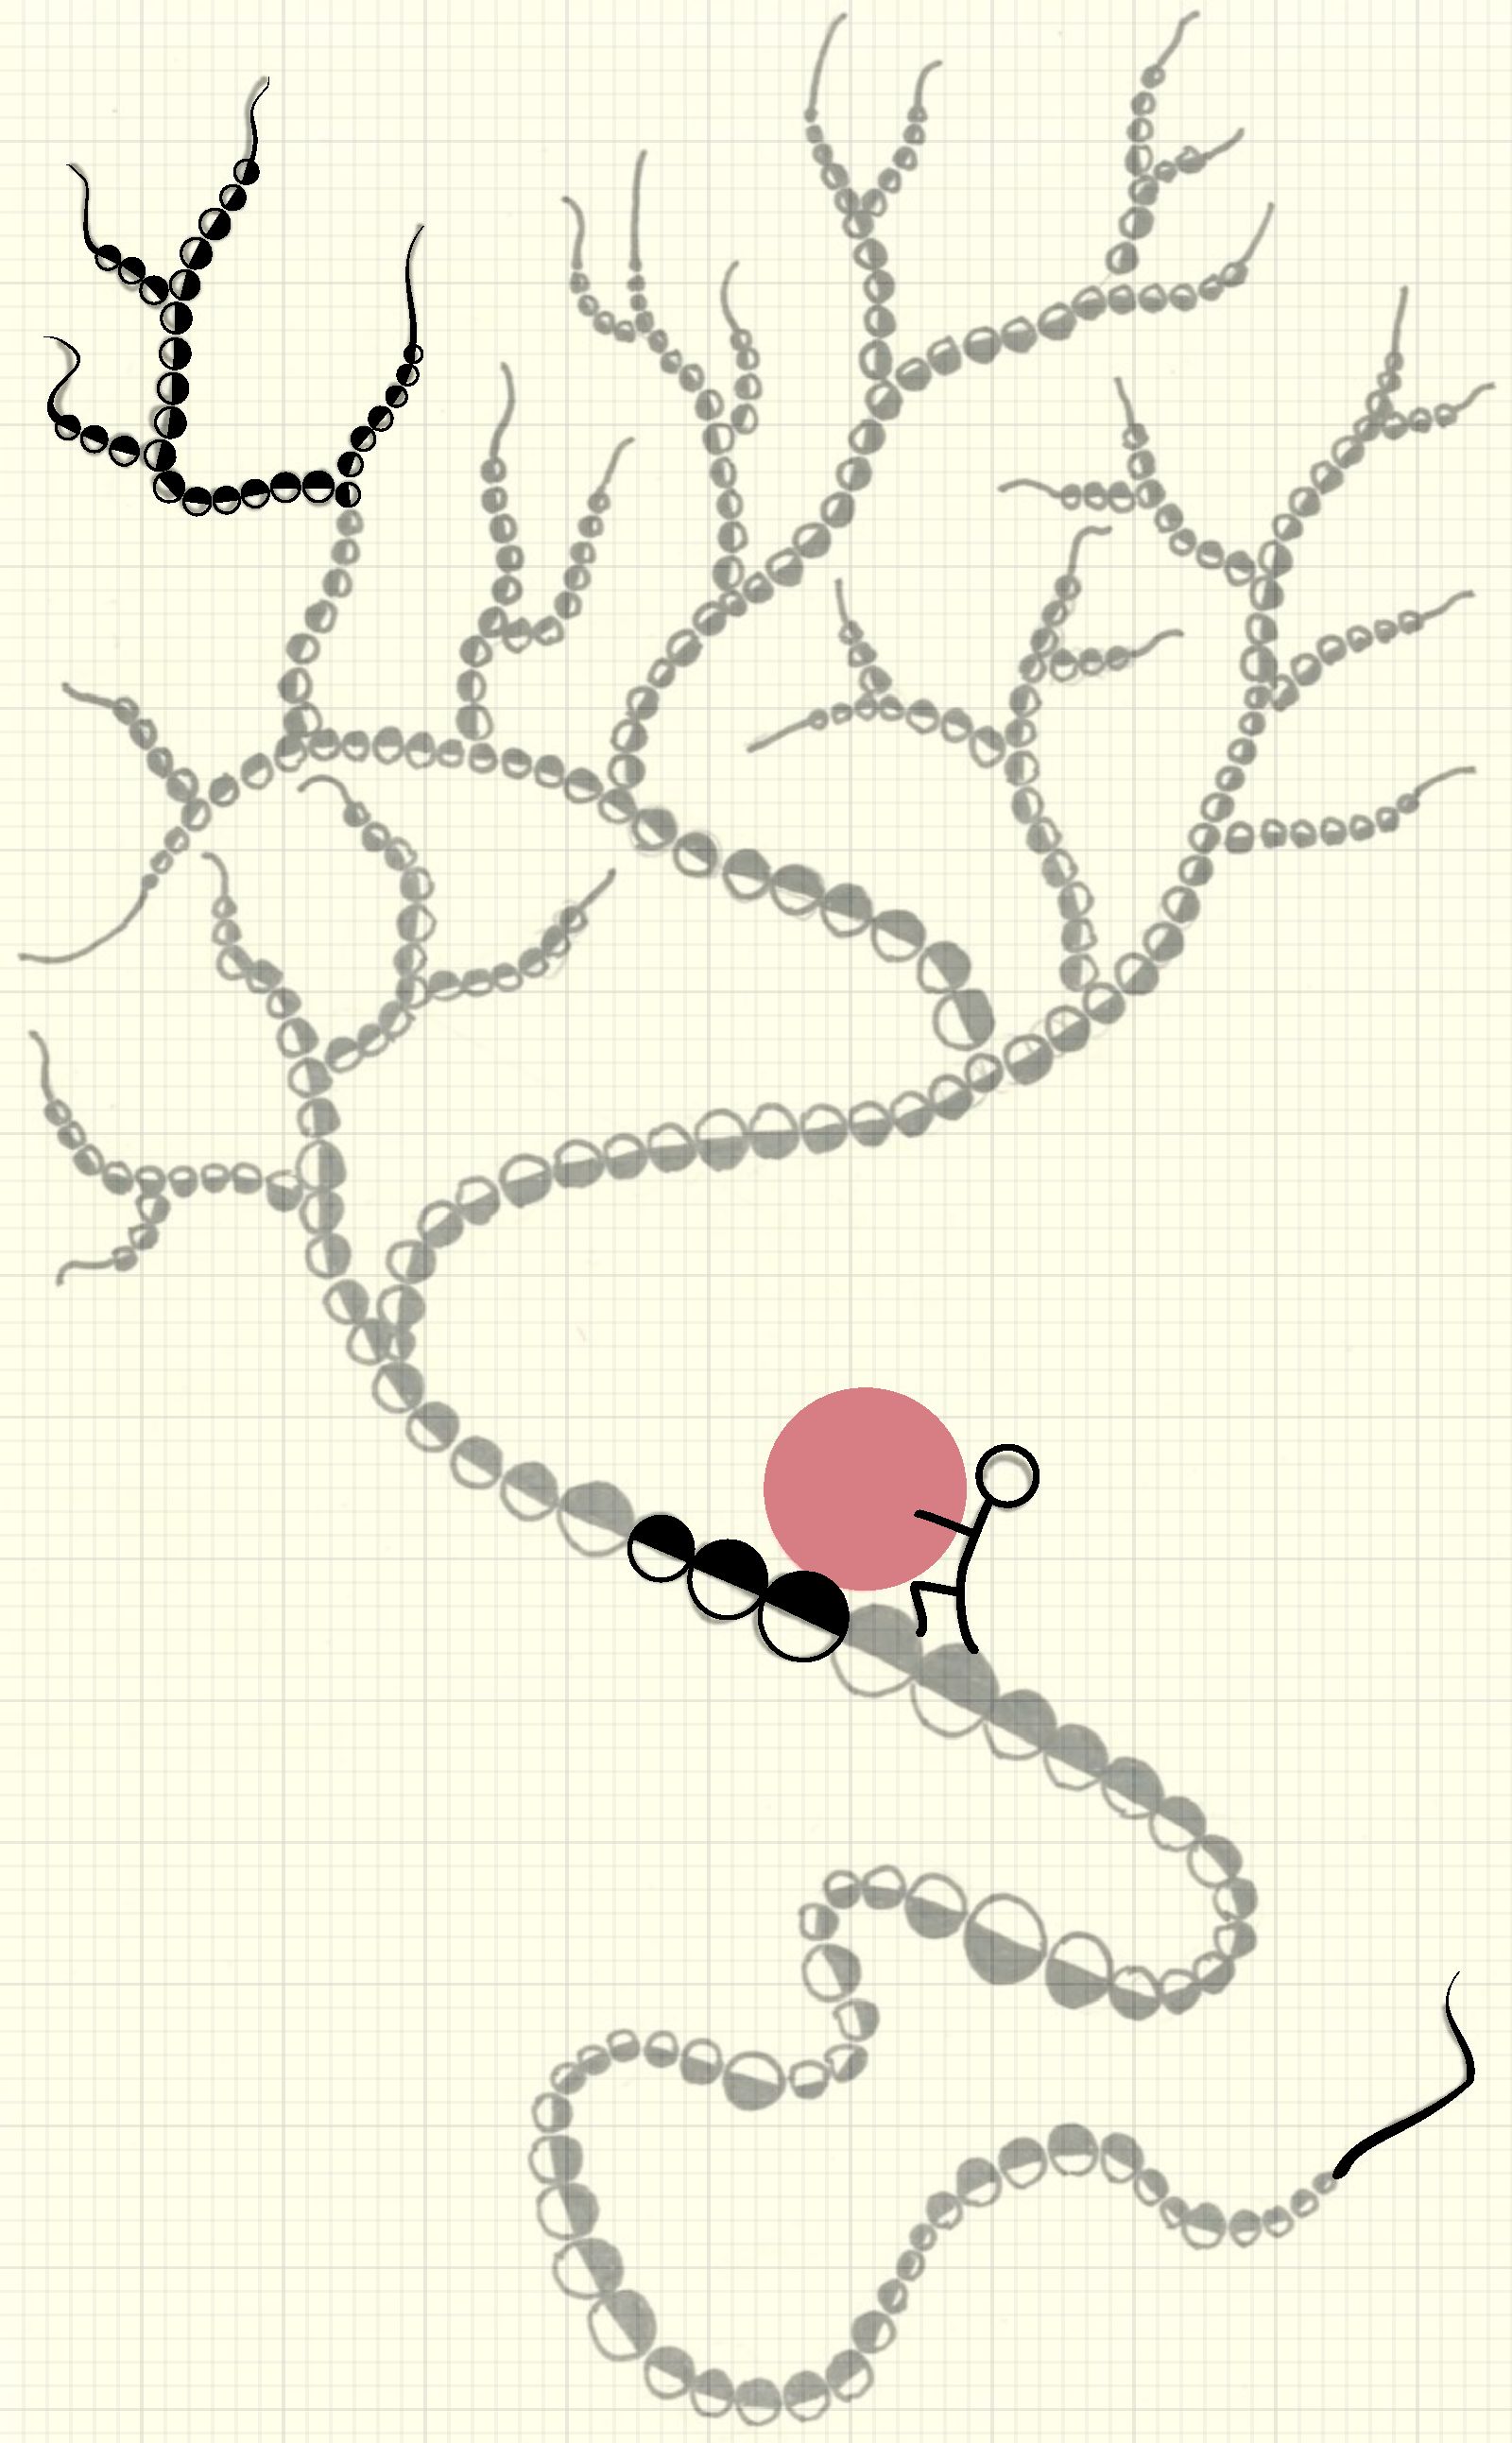
\includegraphics[height=1.23\linewidth]{./cover/syziphus}
\end{center}

%\begin{flushright}
%	{\huge Miroslav Radojevi\'{c}}
%\end{flushright}

\begin{textblock*}{\textwidth}(11cm,24cm)
	{\huge Miroslav Radojevi\'{c}}
\end{textblock*}

\end{changemargin}

%\clearpage
%\restoregeometry
%}
% ************************************************************************
%
% Title Page
%
% ************************************************************************

\setlength{\parindent}{0pt}
\thispagestyle{empty}

%\pagecolor{white} % in case previous page had the background color

\begin{center}
  \vspace*{5mm}
  {\huge\bf Methods for Automated\\[0.3ex] Neuron Image Analysis\\}
  \vspace{12.85cm}
  {\large\bf Miroslav Radojevi\'{c}}
\end{center}
\setlength{\parindent}{\myindent}



% ************************************************************************
%
% Colophon
%
% ************************************************************************

\newpage
\setlength{\parindent}{0pt}
\thispagestyle{empty}

\section*{Colophon}
\addcontentsline{toc}{chapter}{Colophon}

\bigskip
This book was typeset by the author using \LaTeX{}2{\LARGE $_{\varepsilon}$}. The main body of the text was set using a 10-points Computer Modern Roman font. All graphics and figures were created using Inkscape (free and open-source) and Autodesk \textsuperscript{\textregistered}Graphic vector graphics editors and included in the book as Portable Document Format (PDF). % ${}^{\textrm{TM}}\!\!$

\bigskip
Cover design by the author.% The graphics on the cover symbolizes the Sisyphus building a neuron tree. We all do Sisyphean work now and then.
\bigskip

\vfill

\includegraphics[height=0.08\textheight]{./logos/emc1}

The research described in this thesis was carried out at the Erasmus MC - University Medical Center Rotterdam (Rotterdam, the Netherlands). 
\bigskip


\includegraphics[height=0.07\textheight]{./logos/nwo-nl}

\bigskip

%\rule[0.8mm]{\textwidth}{0.3mm}
Copyright \copyright\ 2018 by Miroslav Radojevi\'{c}. All rights reserved. No part of this publication may be reproduced or transmitted in any form or by any means, electronic or mechanical, including photocopy, recording, or any information storage and retrieval system, without permission in writing from the author.

\bigskip
ISBN 000-00-0000000-0
\bigskip
Printed by ABC Company
\setlength{\parindent}{\myindent}
% ************************************************************************


% ************************************************************************
%
% Formal page
%
% ************************************************************************

\setlength{\parindent}{0pt}
\thispagestyle{empty}

\begin{center}
  
  \vspace*{5mm}
  {\huge\bf Methods for Automated\\[0.3ex] Neuron Image Analysis\\}

  \vfill
  \vfill
  \vfill

  {\large Methoden voor geautomatiseerde neuronbeeldanalyse\\[1ex]}

%  {\large(met een samenvatting in het Nederlands)}

  \vfill
  \vfill
  \vfill
  \vfill

  {\large\bf Proefschrift}
  {\large 
  \vfill
  \vfill
  
  \normalsize
  
  ter verkrijging van de graad van doctor aan de \\Erasmus Universiteit Rotterdam\\
op gezag van de \\rector magnificus\\
  \vfill
Prof.dr.~S.W.J.~Lamberts\\
  \vfill
en
volgens besluit van het College voor Promoties. 
  \vfill
De openbare verdediging zal plaatsvinden op \\Dag XY maand 20XY om 8:00 uur
  
  
  \vfill
  \vfill
  
  \large
  door}

  \vfill
  \vfill
  \vfill

  {\large\bf Miroslav Radojevi\'{c}}

  \vfill

  {\large geboren te U\v{z}ice, Servi{\"e}}

  \vfill
  \vfill

\includegraphics[width=0.3\textwidth]{./logos/emc}
\end{center}

% ************************************************************************

\newpage
\thispagestyle{empty}
\label{othersideformal}

\begin{tabular}{@{}ll@{}}
\large\bf{Promotiecommissie} &\\ [8ex]
Promotor:    & {\bf Prof.dr.~W.J.~Niessen}\\[3ex]
Overige leden: & {\bf Prof.dr.ir.~H.H.~Weinans}\\[1ex]
&{\bf Dr.ir.~N.J.~Galjart}\\[1ex]
&{\bf Dr.~J.-C.~Olivo-Marin}\\[3ex]
Copromotor: & {\bf Dr.ir.~H.W.~Meijering}\\
\end{tabular}

% \vfill
% %\rule[0.8mm]{100mm}{0.3mm}\hfill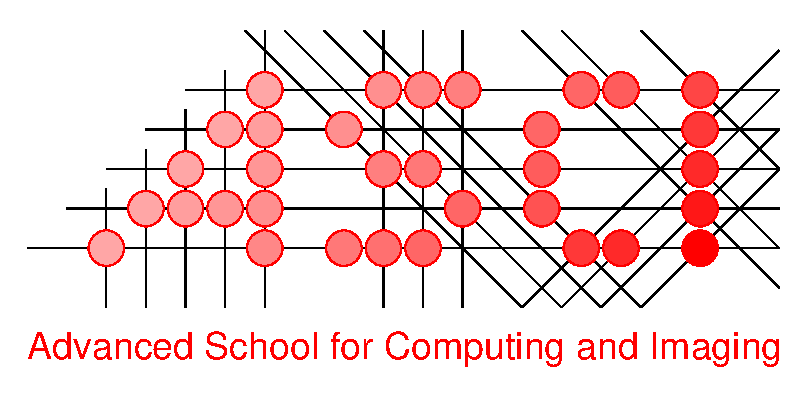
\includegraphics[width=0.20\textwidth]{./asci.eps}
% \rule[0.8mm]{\textwidth}{0.3mm}

% %\bigskip

% The research described in this thesis was carried out at the Erasmus MC -- University Medical Center Rotterdam (Rotterdam, the
% Netherlands), under the auspices of the Advanced School for Computing and Imaging (ASCI). This work was financially supported by the Netherlands Organization for Scientific Research (NWO) through VIDI-grant 639.022.401.

% \bigskip

%Financial support for publication of this thesis was kindly provided by Vital Images Inc.\ (USA), Philips Medical Systems Nederland B.V., SGI Nederland, and Schering Nederland B.V. Financial support by the Netherlands Heart Foundation and the R\"ontgen Stichting Utrecht is also gratefully acknowledged.  Additional financial support was provided by the Image Sciences Institute and Utrecht University.

\setlength{\parindent}{\myindent}

% ************************************************************************


% ***********************************************************************
%
% Preface
% 
% ***********************************************************************

\chpos{14mm}{10mm}
\chapter*{Preface}
\markboth{Preface}{Preface}
\addcontentsline{toc}{chapter}{Preface}

This thesis describes the research carried out as part of my Ph.D. study at the Erasmus University Medical Center Rotterdam. Over the number of ascetic years devoted to exploration and learning, I have learned much not only about the specific field, but also helped me shaping up the view on the reserach and the life and, for the most part, overcoming the obstacles.

I have to acknowledge the . 

I am grateful to my supervisor Erik Meijering.

\bigskip
\begin{flushright}
  \begin{tabular}{@{}l@{}}
    Miroslav Radojevi\'{c}\\
    Rotterdam, January 2019.
  \end{tabular}
\end{flushright}
% ************************************************************************

% ************************************************************************
%
% Table of Contents
%
% ************************************************************************

\noquote
\chpos{17mm}{16mm}
\tableofcontents
\cleardoublepage
% ************************************************************************

%%% Local Variables: 
%%% mode: latex
%%% TeX-master: "phdthesis"
%%% End: 

%\glsaddall
%\printglossaries
%\printglossary[style=long]
\printglossary[style=long,type=\acronymtype,title={List of Abbreviations}]

% ************************************************************************
\pagenumbering{arabic}
\setcounter{page}{1}

\graphicspath{{./chapter1/}}
% ************************************************************************
%
% Introduction
%
% ************************************************************************
\chpos{22mm}{10mm}

\chapter[Introduction]{Introduction}
\markboth{\thechapter\ \ Introduction}{\thechapter\ \ Introduction}
\label{ch1:introduction}

%\mysquote{0.8\textwidth}{Quote text.}{Author (\oldstylenums{1000} - \oldstylenums{1100})}

% ************************************************************************
% sources:
% https://www.quantamagazine.org/why-the-first-drawings-of-neurons-were-defaced-20170928/
% https://www.npr.org/sections/health-shots/2017/01/26/511455876/art-exhibition-celebrates-drawings-by-the-founder-of-modern-neuroscience
% https://www.nytimes.com/2018/01/18/arts/design/brain-neuroscience-santiago-ramon-y-cajal-grey-gallery.html
% https://www.brainpickings.org/2017/02/23/beautiful-brain-santiago-ramon-y-cajal/
\section{Neuron cell reconstruction} 
\lettrine{F}{ascination} with the neuron cells dates to the time when the glance into the sample of the silver-stained neuronal brain tissue over a century ago made it possible to gain insight into the intricate network that forms the very essence of the nervous system. The remarkable and groundbreaking drawings of Santiago Ram\'{o}n y Cajal \cite{swanson2017,ramon2008histologia}, neuroscience founding father, remain today as vivid as and fresh as the images captured by the latest fluorescence microscope, processed and rendered with the novel computer software. Ever since the discovery of the \textit{neuron doctrine}\footnote{Every neuron in the brain is separate. Neurons conduct information in a defined direction and communicate across the synapses.} \cite{glickstein2006golgi} and the early hand-made illustrations of the microscope-magnified samples of the brain tissue, numerous scientists and researchers of various backgrounds and interests have been trying to gain a deeper insight into the nervous system and the captivating mechanism of, arguably, one of the most complex and mysterious organs - brain. Numerous technical obstacles stand out when reaching out to such vastly unknown world, primarily due to the physical inaccessibility and the generally intangible nature of the whole system. Neuron cell thus represents a core building block of the brain and the nervous system. It appears in variety of shapes and specializations \cite{ascolitrees}. The estimated number of neuron cells in a human brain amounts to 89 billion \cite{herculano2009human} - number comparable to the count of stars in the Milky Way galaxy. Each neuron \textit{add: neuron dimensions} is further connected to 50 thousand other neurons on average which results in a very powerful computational network and an extremely efficient information storage. Captivating mechanism of the brain is an everlasting research topic as the complex functionality of the brain defines much of the activities, even the those such as consciousness. Discovering how the brain works is one of the grand unanswered questions of our era and central to diverse fields such as physics, mathematics, biology and recently prominent - computer science.

Nervous system activity is also manifested with the physical appearance of its neuron cells. Morphology of the single cell, shape of the neuronal network, topology or connectivity react to the external conditions or external stimuli. With the imaging tools such as fluorescence microscopy, the physical appearance the morphology of the single cell can be captured at micro meter scale can be inspected and recorded. Indeed, the studies that require deeper analysis make use of the imaging techniques that can reach nano meter scale, such as electron microscopy. In other words, accurate quantification of the cell shape is an important step towards better understanding of the cell functionality. Quantification of the neuronal structure is crucial in many neuroscience studies \cite{halavi2012digital} and quantification from microscopic images is identified as one of the major technical challenges in the digital era of neuroscience \cite{peng2015diadem}.

The advancements in informatics made it possible (Fig.~\ref{ch1__fig1}) to utilize computers to solve the neuroinformatics challenges over recent decades. With the ever growing amount of data, the processing of the information remains a challenge.   

\begin{figure}
	\begin{center}
		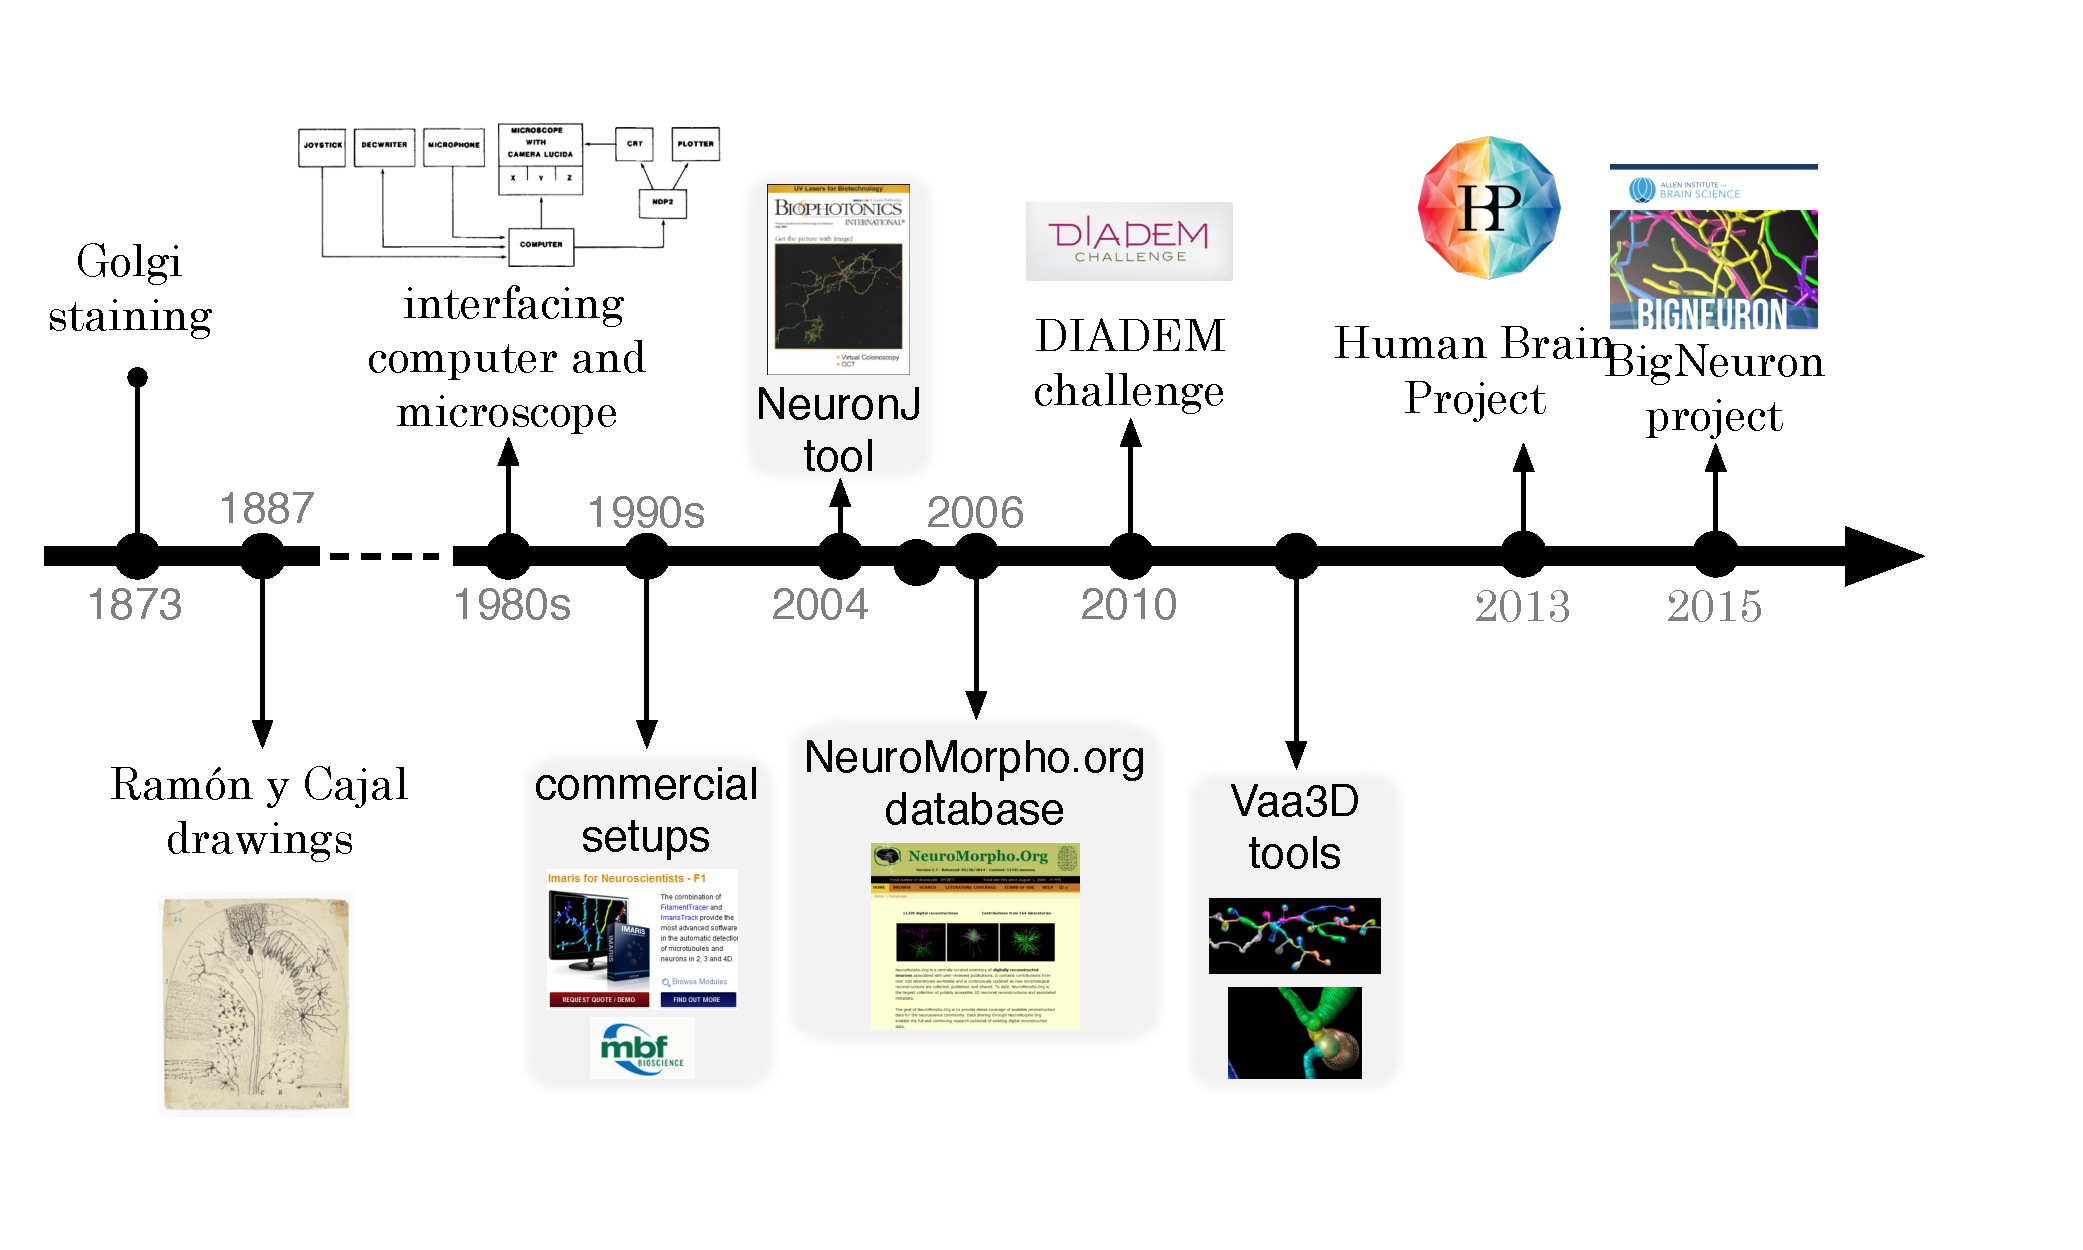
\includegraphics[width=\textwidth]{ch1_fig1}
	\end{center}
	\vspace{-3ex}
	\caption{Brief history of the neuron reconstruction. \textit{Corrections: Cajal drawings as separate item, and dating 1887-1892.}}
	\vspace{-1ex}
	\label{ch1__fig1}
\end{figure}

\section{Essential obstacles in neuron reconstruction}
The key obstacles concerning the full, accurate and robust automation of the neuron reconstruction \cite{meijering2010neuron,donohue2011automated,acciai2016automated} can be seen through the number of factors.

\textit{Morphology} the structural ambiguities of the diverse neuron cells (Fig.~\ref{}) often intractable to the human visual comprehension.

\textit{Noise} noisy image input (imaging on the boundary of the resolution limits in case of the light microscopy).

\textit{Data size} ever increasing size of the image volume needed to be correctly processed in reasonable time.

Aforementioned factors impose much of the computational barrier \cite{peng2011proof,svoboda2011past} in attempt to consistently produce human-comparable digital reconstructions. The real datasets, therefore, commonly leave with the persisting need for human expert assistance to obtain the optimal output. 

\section{Neuron tracing in fluorescence microscopy images}
%One of the key Java tools is the ImageJ library \cite{abramoff2004image}. 

\subsection{Extracting the correct tree}

\subsection{Bayesian methods in neuron tracing}

\begin{figure}
\begin{center}
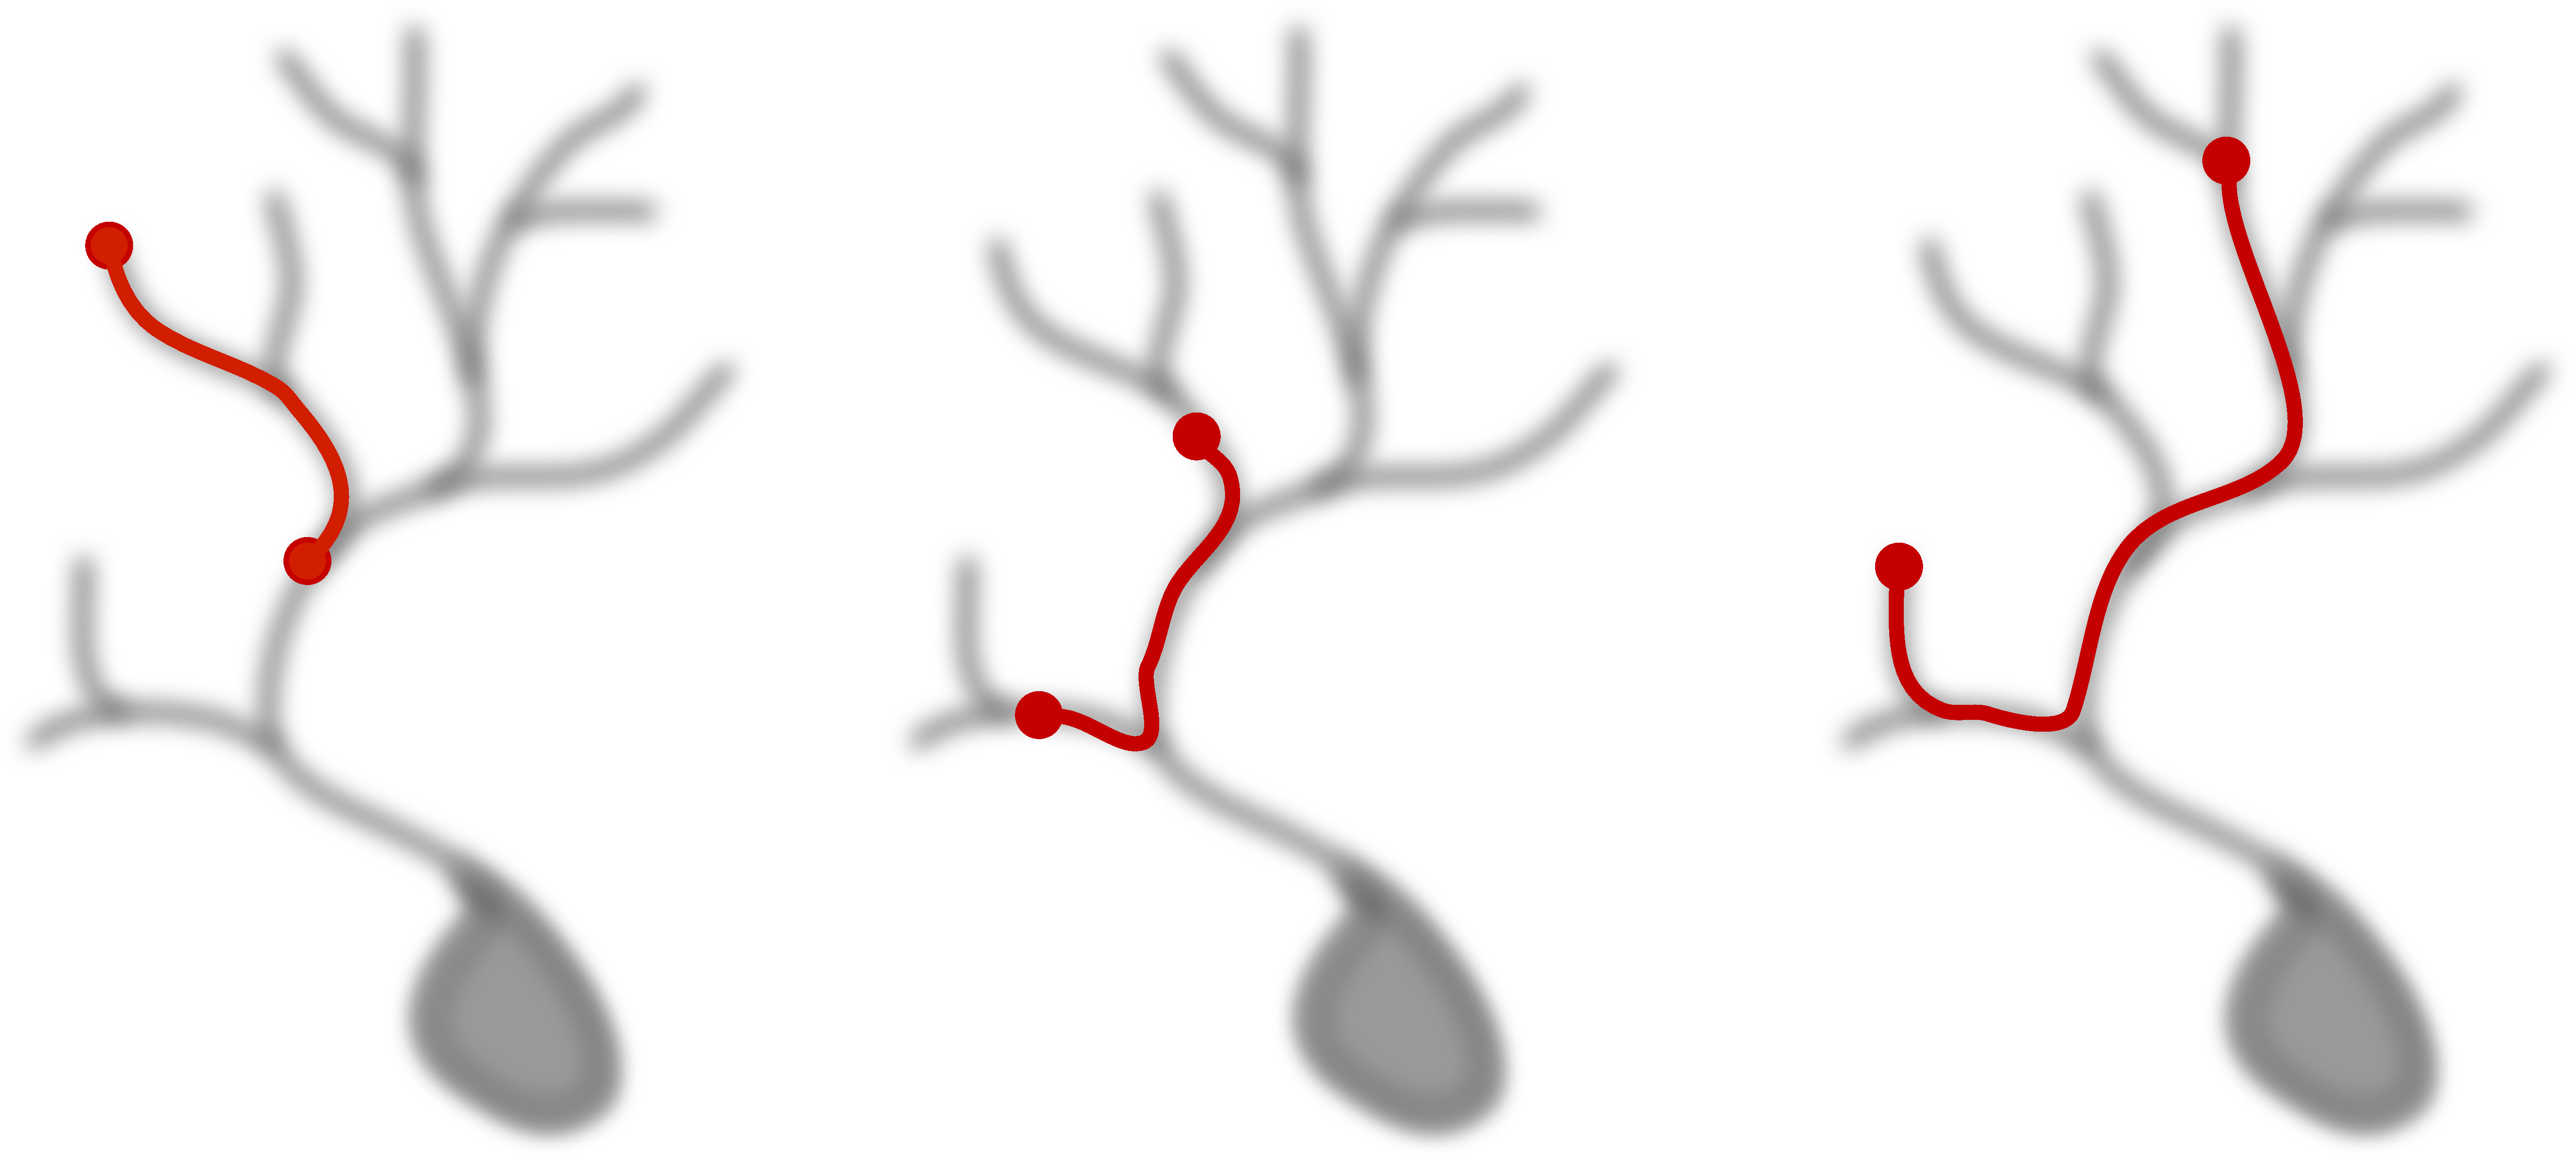
\includegraphics[width=0.5\textwidth]{ch1_fig2}\\
a) Shortest path tracing \\
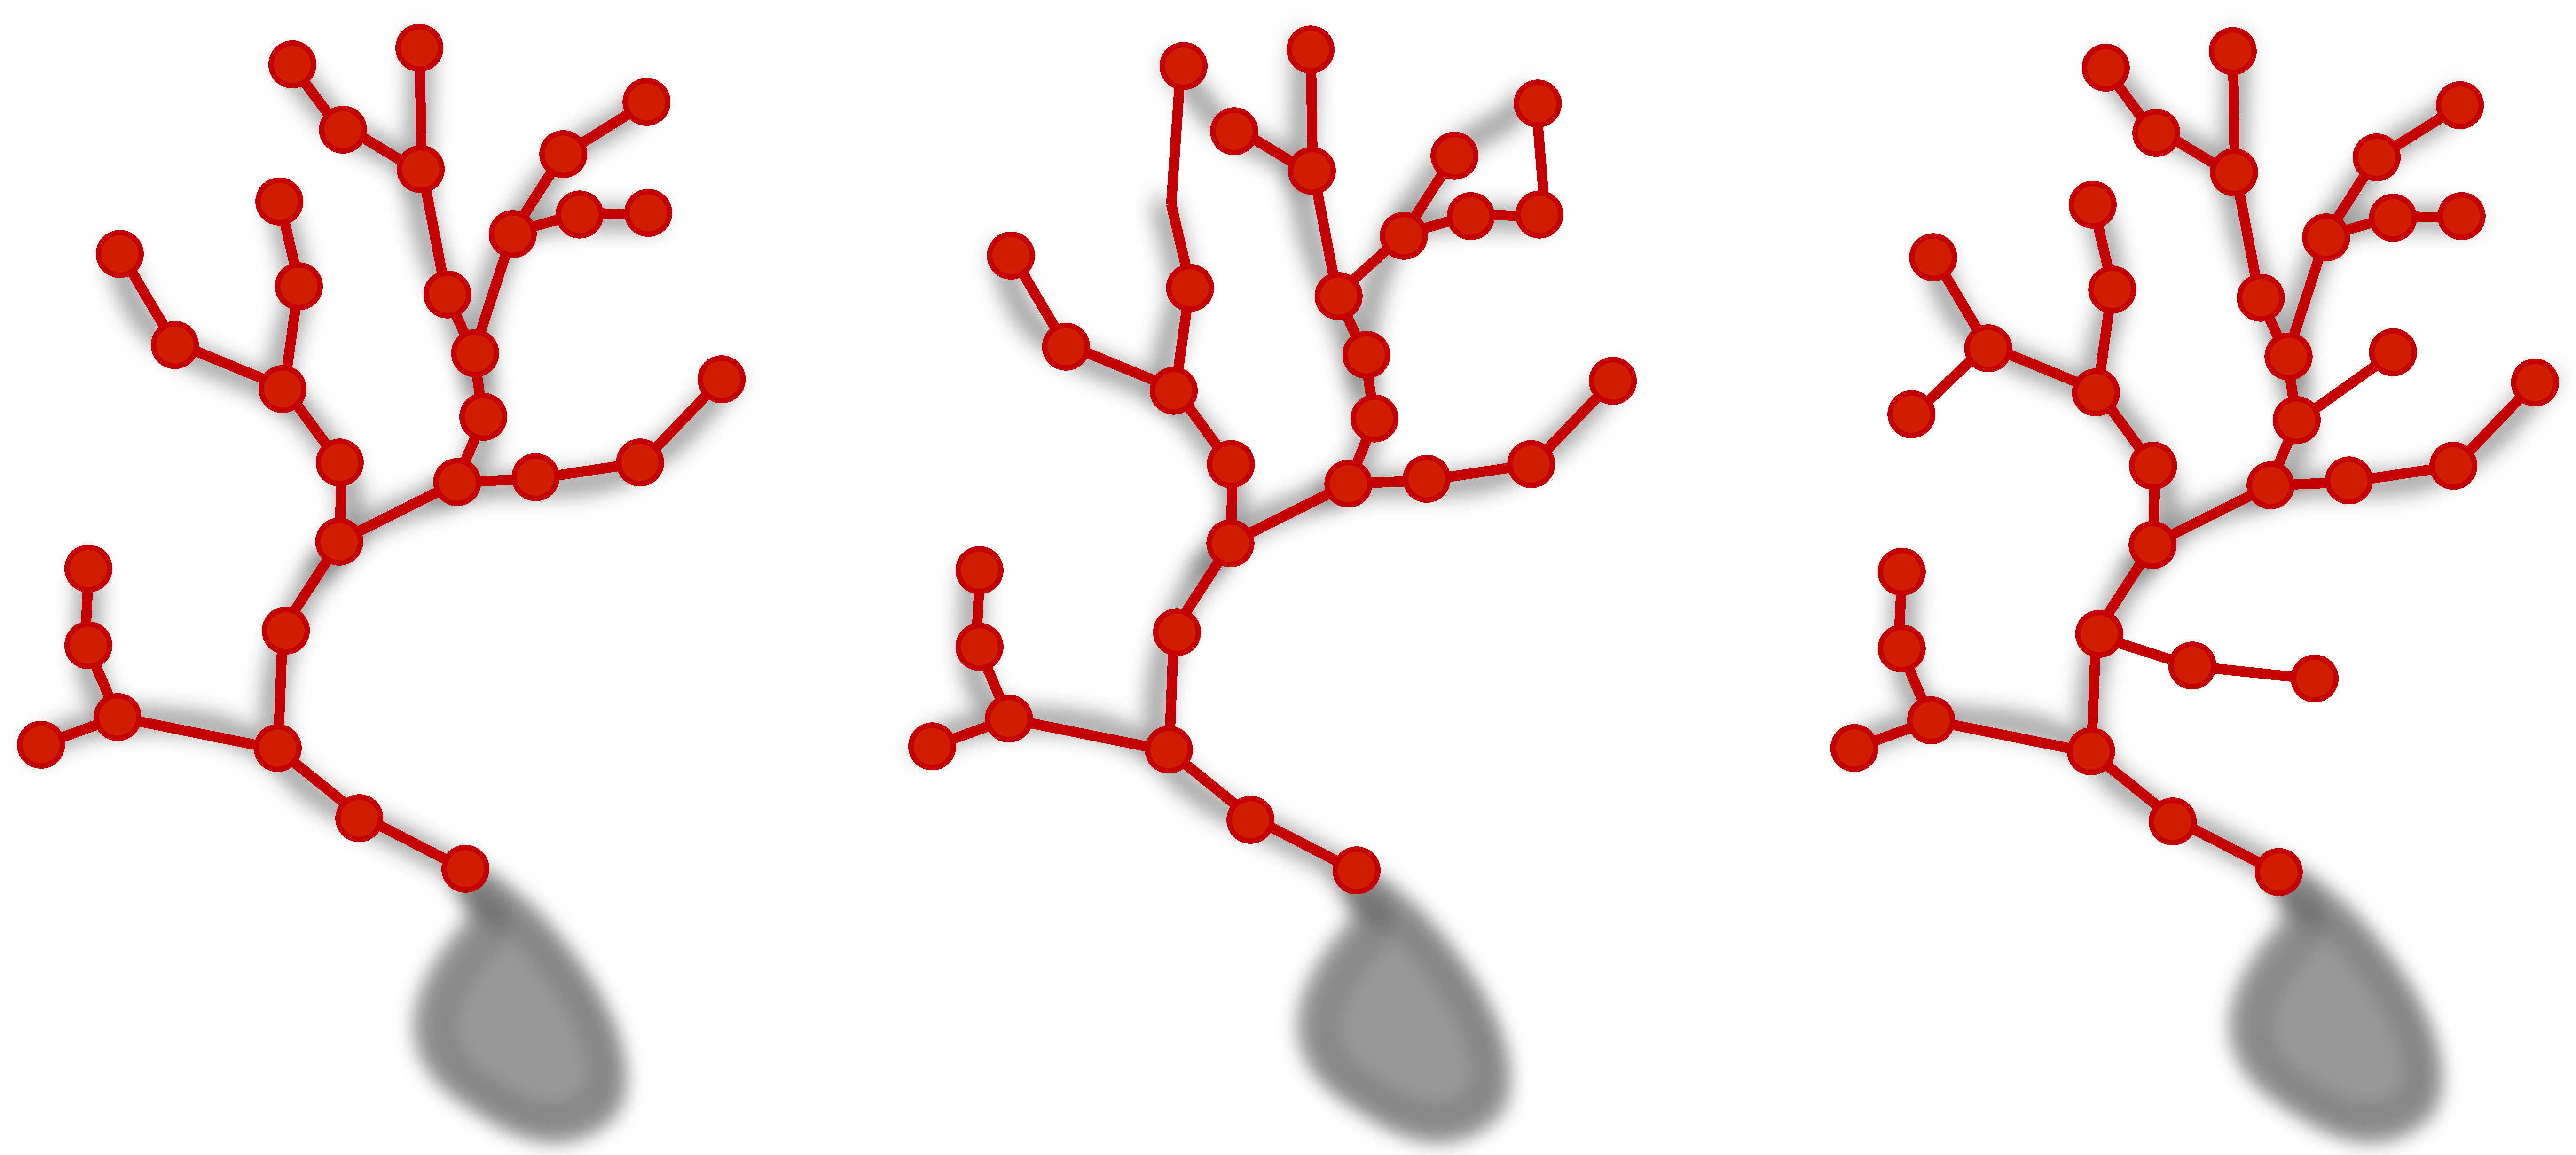
\includegraphics[width=0.5\textwidth]{ch1_fig3}\\
b) Minimum spanning tree \\
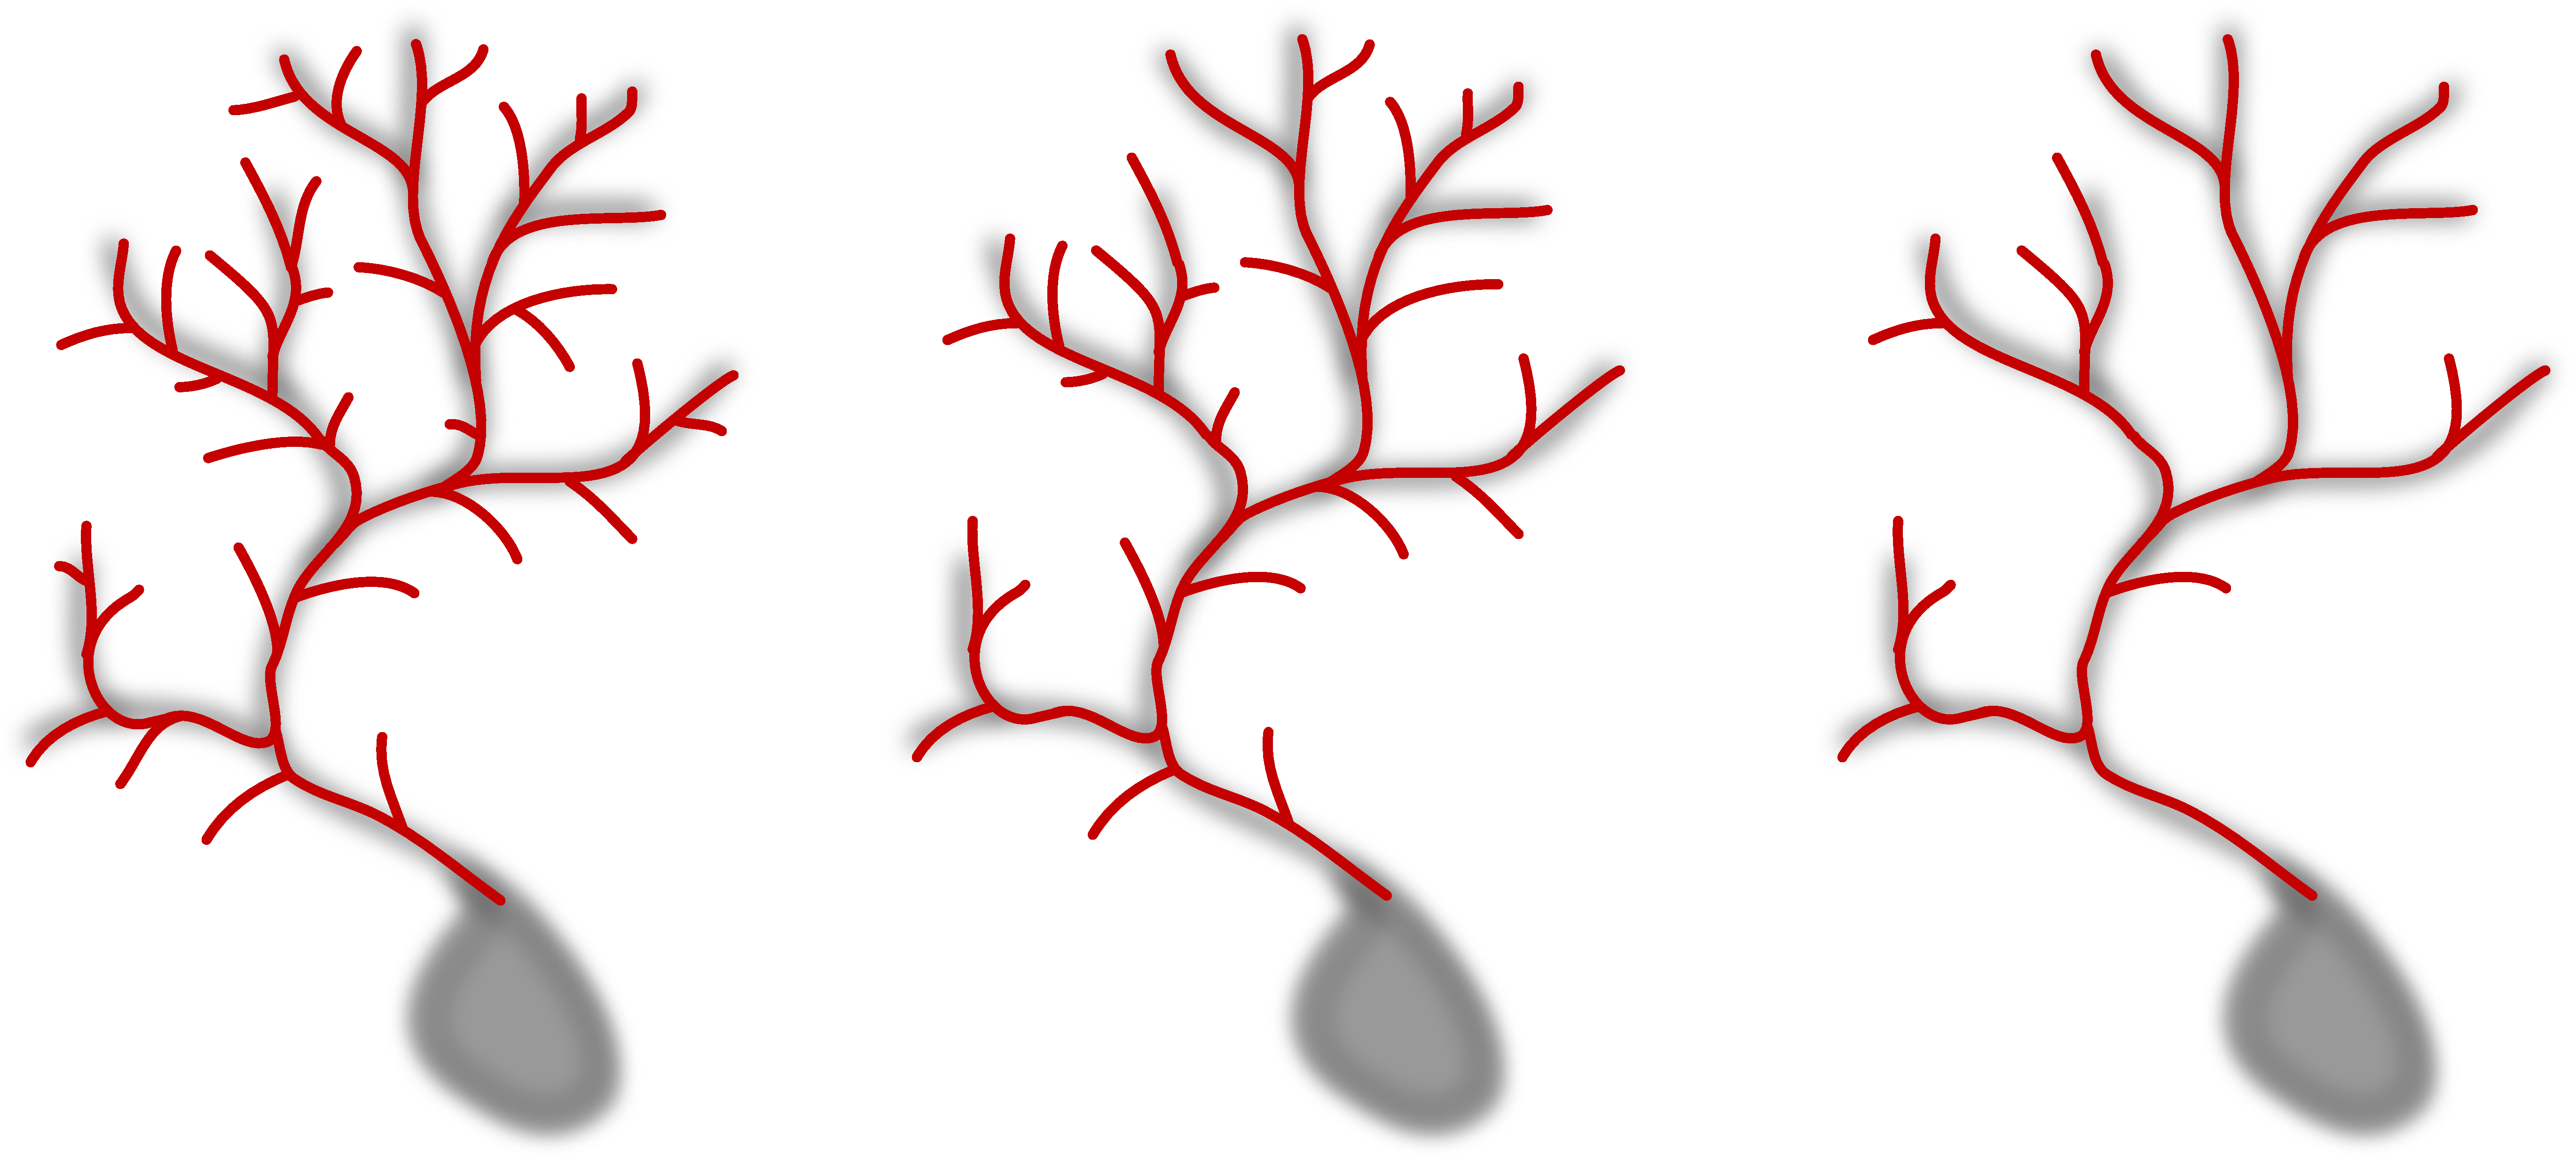
\includegraphics[width=0.5\textwidth]{ch1_fig4}\\
c) Path-prunning
\end{center}
\vspace{-3ex}
\caption{Examples of key neuron reconstruction strategies: a) Finding optimal path between two fixed points, b) Inferring the  optimal tree structure from the given nodes c) Prunning the overcomplete neuron tree.}
\vspace{-1ex}
\label{ch1__fig2-4}
\end{figure}

Computation methods

\section{Examining the neuronal reconstructions}
Once computed, neurons are typically stored in vectorized SWC format. 
\subsection{SWC} 
% source:
% https://www.neuron.yale.edu/phpBB/viewtopic.php?t=3477
%Stockley, E. W.; Cole, H. M.; Brown, A. D. & Wheal, H. V.
%A system for quantitative morphological measurement and electronic modelling of neurons: three-dimensional reconstruction.
%J Neurosci Methods, 1993, 47, 39-51
%
% http://www.neuromorpho.org/myfaq.jsp (What is SWC format?)
% http://research.mssm.edu/cnic/swc.html
% http://www.neuronland.org/NLMorphologyConverter/MorphologyFormats/SWC/Spec.html
The SWC \cite{cannon1998line} is widely used open format for digital neuron reconstruction that describes a reconstruction as a list of 3D nodes (neuronal compartments) with seven attributes (NeuroMorpho.org):  $i$: node index identifier, node type $[0-7]$, node 3D coordinates $(x_i,y_i,z_i)$, radius $(r_i)$ and a parent node index - link towards the predecessor parent node $(j | j=-1)$ if the node has no parent soma node, Fig.~\ref{ch1__fig5}. To define a correct tree structure, each node can only have one predecessor (parent) and the parent node should have lower index so that the indexes of the reconstruction are sorted. Loops and disconnected branches should not exist. The originating node has parend  Etymologically, SWC represents the acronym containing the initials of the last names of Stockley, Wheal, and Cole. Although not directly described in their joint work on quantitative measurement and modeling of the neuron morphology \cite{stockley1993system}, the origin of the SWC name is an acronym of the initials of their last names. Moreover, there is slight uncertainty on the SWC format, especially concerning the unified definition on how soma reconstruction is addressed, so that several variations over the SWC standard can be found\footnote{}.
\begin{figure}
	\begin{center}
		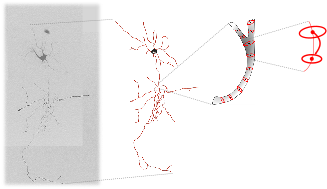
\includegraphics[width=\textwidth]{ch1_fig5} \\
		a 
	\end{center}
	\vspace{-3ex}
	\caption{SWC format of the digital reconstruction. Visualization using Vaa3D \cite{peng2010automatic}}
	\vspace{-1ex}
	\label{ch1__fig5}
\end{figure}

%\begin{figure}[t!]
%	\centering\tiny
%	\begin{tabular}{@{}c@{\hspace{0.02\columnwidth}}c@{\hspace{0.02\columnwidth}}c@{}}
%		& \hspace{3.5em}S = 2 & \hspace{3.5em}S = 3 \\[0.02\columnwidth]
%		\rotatebox{90}{\hspace{0.5em}COR = 0} &
%		\includegraphics[align=c,width=0.47\columnwidth]{synFSnrS2Cor0} & % ./fig/exp.syn/compare_snr/_F(snr,S=2,cor=0)
%		\includegraphics[align=c,width=0.47\columnwidth]{synFSnrS3Cor0} \\ % ./fig/exp.syn/compare_snr/_F(snr,S=3,cor=0)
%		\\[0.01\columnwidth]
%		\rotatebox{90}{\hspace{0.5em}COR = 1} &
%		\includegraphics[align=c,width=0.47\columnwidth]{synFSnrS2Cor1} & % ./fig/exp.syn/compare_snr/_F(snr,S=2,cor=1)
%		\includegraphics[align=c,width=0.47\columnwidth]{synFSnrS3Cor1} % ./fig/exp.syn/compare_snr/_F(snr,S=3,cor=1)
%	\end{tabular}
%	\caption{Average F score of the methods for the synthetic images as a function of SNR. Examples are shown for COR = 0 (top) and 1 (bottom) in combination with S = 2 (left) and 3 (right).}
%	\label{fig:f[snr]_synthetic}
%\end{figure}

\subsection{Measuring distances between neurons}

L-measure, neuro-blast
Distances between neurons can be based on the overlap and the inter-node metric distances.

\section{Thesis outline}
In this thesis probabilistic and bayesian methods are explored.


\graphicspath{{./chapter2/}}
% ************************************************************************
% 
% Fuzzy-Logic Based Detection and Characterization of Junctions and Terminations 
% in Fluorescence Microscopy Images of Neurons
%
% ************************************************************************
\chpos{15mm}{8mm}
\chapter[Fuzzy-Logic Based Detection and Characterization of Junctions and Terminations in Fluorescence Microscopy Images of Neurons]{Fuzzy-Logic Based Detection and Characterization of Junctions and Terminations in Fluorescence Microscopy Images of Neurons}
\chaptermark{Fuzzy-Logic Based Detection of Junctions and Terminations}
\label{ch2:fuzzy}
% abstract
{\small \lettrine{D}{igital} reconstruction of neuronal cell morphology is an important step toward understanding the functionality of neuronal networks. Neurons are tree-like structures whose description depends critically on the junctions and terminations, collectively called critical points, making the correct localization and identification of these points a crucial task in the reconstruction process. In this chapter, a fully automatic method for the integrated detection and characterization of both types of critical points in fluorescence microscopy images of neurons is presented. In view of the majority of our current studies, which are based on cultured neurons, the method was described and evaluated for application to two-dimensional (2D) images. The method relies on directional filtering and angular profile analysis to extract essential features about the main streamlines at any location in an image, and employs fuzzy logic with carefully designed rules to reason about the feature values in order to make well-informed decisions about the presence of a critical point and its type. Experiments on simulated as well as real images of neurons demonstrate the detection performance of our method. A comparison with the output of two existing neuron reconstruction methods reveals that our method achieves substantially higher detection rates and could provide beneficial information to the reconstruction process.\par}
\vspace*{11em}
% ************************************************************************
\begin{publish}
Based upon: M. Radojevi\'{c}, I. Smal, E. Meijering, ``Fuzzy-Logic Based Detection and Characterization of Junctions and Terminations in Fluorescence Microscopy Images of Neurons'', \textit{Neuroinformatics}, vol. 11, no. 11, pp.1-11, 2015.   
\end{publish}

\section{Introduction}
\label{sec:introduction}
The complexity and functionality of the brain depend critically on the morphology and related interconnectivity of its neuronal cells \cite{kandel2000principles, ascoli2002computational, donohue2008comparative}. To understand how a healthy brain processes information and how this capacity is negatively affected by psychiatric and neurodegenerative diseases \cite{anderton1998dendritic, lin2010mechanisms, vsivskova2014dendritic} it is therefore very important to study neuronal cell morphology. Advanced microscopy imaging techniques allow high-sensitivity visualization of individual neurons and produce vast amounts of image data, which are shifting the bottleneck in neuroscience from the imaging to the data processing \cite{svoboda2011past, peng2011proof, senft2011brief, halavi2012digital} and call for a high level of automation. The first processing step toward high-throughput quantitative morphological analysis of neurons is their digital reconstruction from the image data. Many methods have been developed for this in the past decades \cite{meijering2010neuron, donohue2011automated} but the consensus of recent studies is that there is still much room for improvement in both accuracy and computational efficiency \cite{liu2011diadem, svoboda2011past}.

A key aspect of any neuron reconstruction method is the detection and localization of terminations and junctions of the dendritic (and axonal) tree, collectively called ``critical points'' throughout this chapter (Fig.~\ref{fig1}), which ultimately determine the topology and faithfulness of the resulting digital representation. Roughly there are two ways to extract these critical points in neuron reconstruction \cite{al2008improved, meijering2010neuron, basu2013segmentation}. The most often used approach is to start with segmentation or tracing of the elongated image structures and then to infer the critical points, either afterwards or along the way, by searching for attachments and endings in the resulting subsets \cite{dima2002automatic, xiong2006automated, narro2007neuronmetrics, vasilkoski2009detection, bas2011principal, chothani2011automated, Dehmelt-2011, ho2011neurphologyj, choromanska2012automatic, xiao2013app2}. This approach depends critically on the accuracy of the initial segmentation or tracing procedure, which usually is not designed to reliably capture critical points in the first place and thus often produces very fragmented results, requiring manual postprocessing to fix issues \cite{peng2011proof, luisi2011farsight, dercksen2014filament}. The reverse approach is to first identify critical points in the images and then to use these as seed points for tracing the elongated image structures. Critical points can be obtained either by manual pinpointing, as in semiautomatic tracing methods \cite{meijering2004design, schmitt2004new, narro2007neuronmetrics, lu2009semi, peng2010v3d, longair2011simple}, or by fully automatic detection using sophisticated image filtering and pattern recognition methods (discussed in the chapter sequel). The latter approach has barely been explored for neuron reconstruction, but if reliable detectors can be designed, they provide highly valuable information to the reconstruction process.

\begin{figure}[!b]
	\centering
	\begin{tabular}{c@{\hspace{1em}}c@{\hspace{1em}}}
		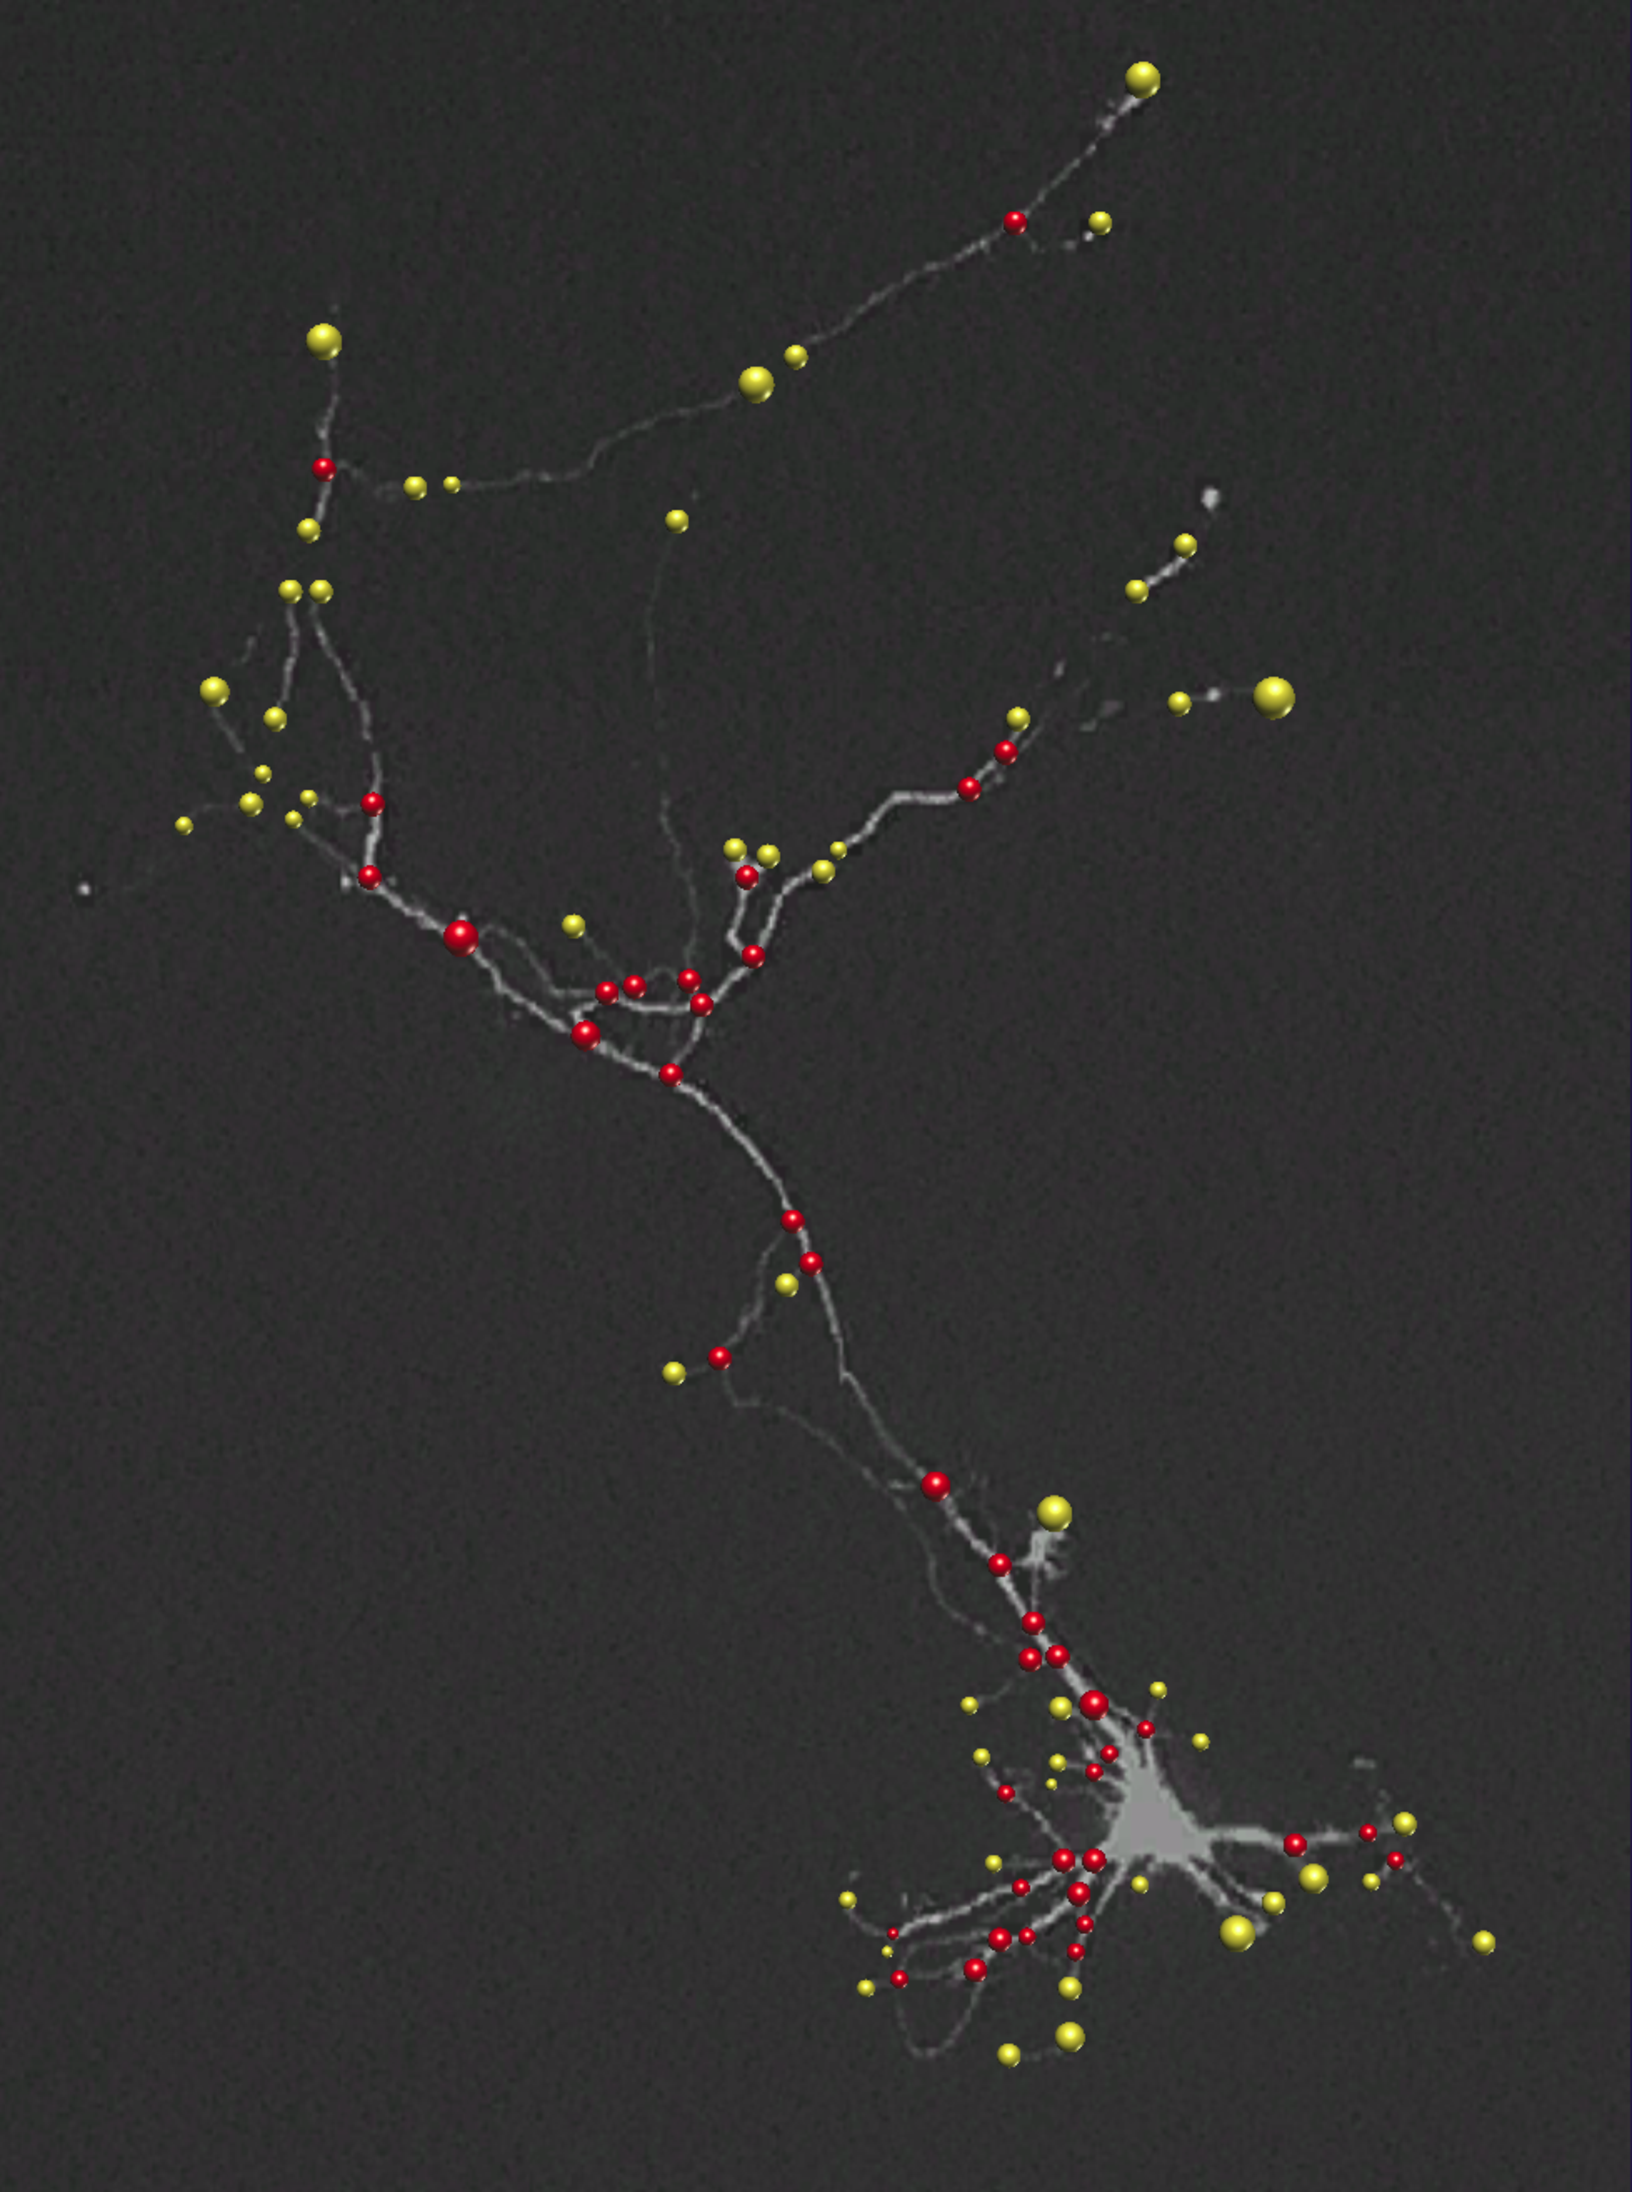
\includegraphics[height=0.65\columnwidth]{fig1} &
		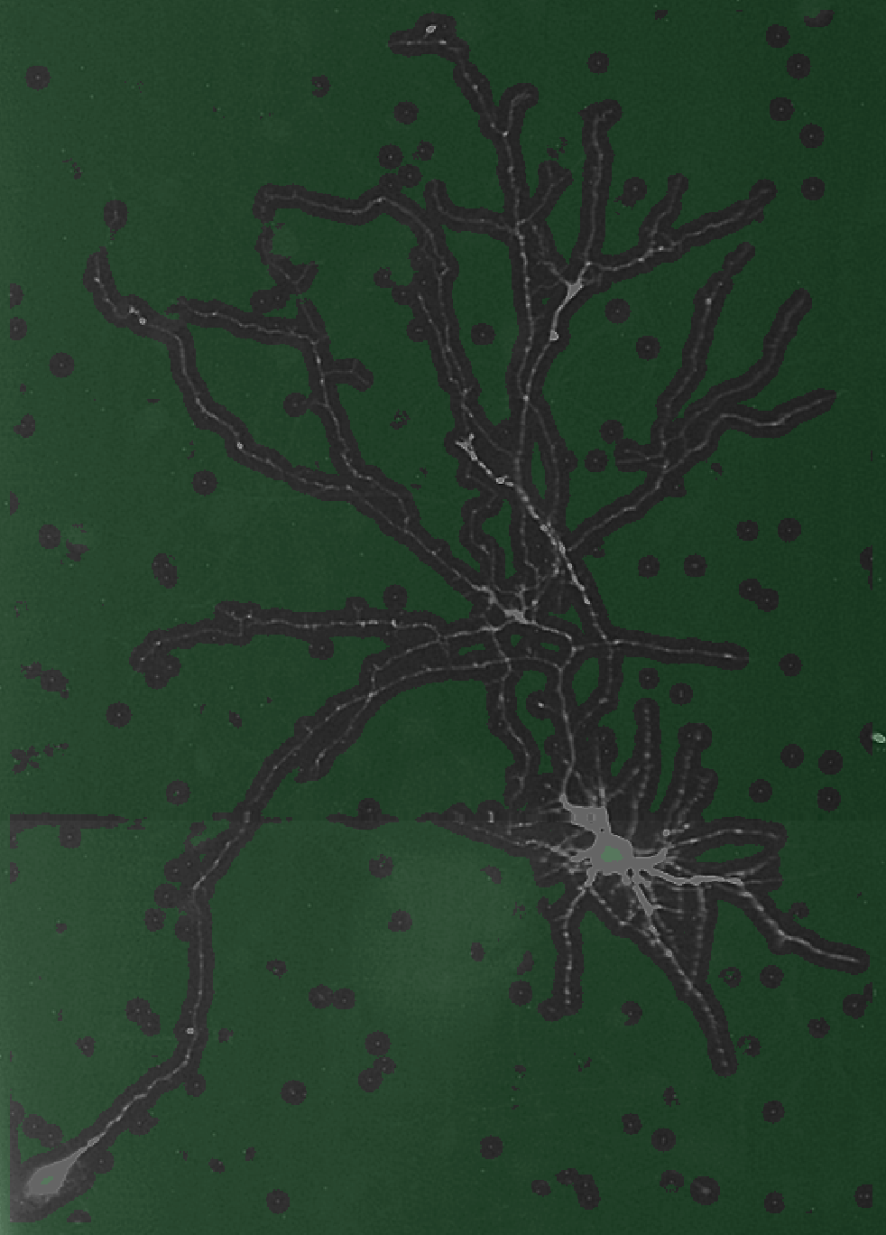
\includegraphics[height=0.65\columnwidth]{fig2} \\
		a) & b) 	
	\end{tabular}
	\caption{a) Fluorescence microscopy image of a neuron with manually indicated junctions (red circles) and terminations (yellow circles). The radius of each annotated critical-point region reflects the size of the underlying image structure. b) Example of foreground selection. The original image of $560\times780$ pixels is divided into background (green transparent mask) and foreground (gray-scale regions without mask) \textit{using} $r_{d}=8$ pixels and the $75^\textrm{th}$ variation percentile as threshold. In this example, 25\% of the total number of pixels is selected for further processing.}
	\label{fig1}
\end{figure}

A novel method is presented - coined Neuron Pinpointer (\gls{np}) - for fully automatic detection and characterisation of critical points in fluorescence microscopy images of neurons. The method is described and evaluated for studies where single (cultured) neurons are imaged in 2D although all aspects of the method can in principle be extended to 3D. The method may also be useful for reconstruction approaches based on 2D projections \cite{zhou2015neuron}. For computational efficiency the method starts with an initial data reduction step, based on local variation analysis, by which obvious background image regions are excluded. In the remaining set of foreground regions the method then explores the local neighborhood of each image pixel and calculates the response to a set of directional filters. Next, an iterative optimization scheme is used for robust peak selection in the resulting angular profile, and a set of corresponding features relevant for the detection task is computed. The feature set is then further processed to make a nonlinear decision on the presence of a critical point and its type (termination or junction) at each foreground image pixel. To conveniently deal with ambiguity and uncertainty in the data, the decision-making is carried out by a fuzzy-logic rule-based system using predefined rules specifically designed for this task. The presented work aims to facilitate the task of automatic neuron reconstruction by contributing a general scheme for extracting critical points that can serve as useful input for any tracing algorithm.

This chapter is a considerably extended version of the conference report \cite{radojevic2014fuzzy}. The filtering algorithms and fuzzy-logic rules had been modified so as to be able to detect both junction and termination points. In addition, the full details of the method are presented here and an extensive evaluation based on both manually annotated real neuron images and computer generated neuron images. To obtain the latter a new computational approach is proposed based on publicly available expert manual tracings. Chapter starts with a brief overview of related work on critical-point detection (Section~\ref{sec:related-work}) and then the underlying concepts (Section~\ref{sec:proposed-method}), implementational details (Section~\ref{sec:implementation-details}), and experimental evaluation (Section~\ref{sec:experiments}) are presented, followed by a summary of the conclusions that can be derived from the results (Section~\ref{sec:conclusions}).

\section{Related Work}
\label{sec:related-work}
Detecting topologically critical points in images has been a long-standing problem in many areas of computer vision. This section provides with a brief review of the problem and proposed solutions in order to put presented work into context.

Examples of previous work include the design of filters to find image locations where either three or more edges join (``junctions of edges'') \cite{sinzinger2008model, hansen2004neural, laganiere2004detection} or three or more lines join (``junctions of lines'') \cite{yu1998rotated, deschenes2000detection}. In biomedical applications, the predominant type of junction is the bifurcation, with occasional trifurcations, as seen in blood vessel trees, bronchial trees, gland ductal trees, and also in dendritic trees \cite{koene2009netmorph, iber2013control}. Hence, research in this area has focused on finding image locations where three (or more) elongated structures join \cite{tsai2004model, agam2005vessel, bevilacqua2005combined, bhuiyan2007automatic, zhou2007vascular, aibinu2010vascular, calvo2011automatic, obaraa2012contrast, su2012junction, azzopardi2013automatic}.

A common approach to find bifurcation points is to infer them from an initial processing step that aims to segment the elongated structures. However, the way these structures are segmented may influence the subsequent critical-point inference. Popular image segmentation methods use intensity thresholding and/or morphological processing, in particular skeletonization \cite{hoover2000locating, dima2002automatic, he2003automated, weaver2004automated, pool2008neuritetracer, bevilacqua2009comparison, leandro2009automatic, aibinu2010vascular}, but these typically produce very fragmented results. Popular methods to enhance elongated image structures prior to segmentation include Hessian based analysis \cite{frangi1998multiscale, xiong2006automated, zhang2007automated, al2008improved, yuan2009mdl, turetken2011automated, myatt2012neuromantic, basu2013segmentation, santamaria2015automatic}, Laplacian-of-Gaussian filters \cite{chothani2011automated}, Gabor filters \cite{bhuiyan2007automatic, azzopardi2013automatic}, phase congruency analysis \cite{obara2012contrast}, and curvelet based image filtering approaches \cite{narayanaswamy20113}. However, being tailored to elongated structures, such filters often yield a less optimal response precisely at the bifurcation points, where the local image structure is more complex than a single ridge.

Several concepts have been proposed to explicitly detect bifurcation points in the images without relying on an initial segmentation of the axonal and dendritic trees. Examples include the usage of circular statistics of phase information \cite{obaraa2012contrast}, steerable wavelet based local symmetry detection \cite{puspoki2013detection}, or combining eigen analysis of the Hessian and correlation matrix \cite{su2012junction}. The problem with existing methods is that they often focus on only one particular type of critical point (for example bifurcations but not terminations), or they use rather rigid geometrical models (for example assuming symmetry), while in practice there are many degrees of freedom \cite{michaelis1994junction}. Image filtering methods for bifurcation detection have also been combined with supervised machine-learning based approaches such as support vector machines \cite{turetken2011automated}, artificial neural networks \cite{bevilacqua2009comparison}, or with multiple classifiers using AdaBoost \cite{zhou2007vascular}, but these lack flexibility in that they require a training stage for each application.

Robust neuron tracing requires knowledge of not only the bifurcation points but also the termination points. Since each type of critical point may vary considerably in terms of geometry (orientation and diameter of the branches) and image intensity (often related to the branch diameter), designing or training a dedicated filter for each possible case is impractical, and a more integrated approach is highly desirable for both detection and characterization of the different types of critical points. To the best of our knowledge, no generic methods currently exist for critical-point detection in neuron images. The method proposed in this chapter aims to fill this gap and to complement exploratory neuron reconstruction algorithms that initialize on a set of seed points.

\section{Proposed Method}
\label{sec:proposed-method}
Proposed method for detection and characterization of critical points consists of three steps: feature extraction (Section~\ref{subsec:feature-extraction}), fuzzy-logic based mapping (Section~\ref{subsec:flrb-detection}), and, finally, critical-point determination (Section~\ref{sec:CPextraction}). Each step is described further in detail. 

\subsection{Feature Extraction}
\label{subsec:feature-extraction}
The aim of the feature extraction step is to compute a set of quantitative features of the local image structure at each pixel position that helps to discriminate between different types of critical points. Since the tree-like neuronal image structures typically cover only a small portion of the image, unnecessary computations are avoided by first performing a foreground selection step (Sec.~\ref{subsubsec:foreground-selection}), which discards image locations that are very unlikely to contain neuronal structures and keeps only those regions that are worthy of further examination. Next, the angular profile (Section \ref{subsubsec:angular-profile}) of each foreground pixel is constructed, from which the quantitative features are computed.

\subsubsection{Foreground Selection}
\label{subsubsec:foreground-selection}
To determine whether a pixel location $(x,y)$ in a given image $I$ should be considered as foreground or background, the local intensity variation $\rho(x,y)$ within a circular neighborhood of radius $r_{d}$ centered at that location is analyzed. To avoid making strong assumptions about the local intensity distribution, the difference between the $95^\textrm{th}$ and the $5^\textrm{th}$ percentile of the intensities within the neighborhood is used as the measure of variation:
\begin{gather} 
\rho(x,y) = \mathcal{P}_{95}(\mathcal{I}_{xy}) - \mathcal{P}_{5}(\mathcal{I}_{xy}) \\
\mathcal{I}_{xy} = \left\{\, I(m,n)\ |\ (m-x)^{2}+(n-y)^{2} \leq r_d^2\, \right\} \\
x,m \in [0,W-1]\ \textrm{and}\ y,n \in [0,H-1]
\end{gather}
where $W$ and $H$ denote, respectively, the width and the height of $I$ in pixels. The value of $\rho$ is relatively low within more or less homogeneous regions (background but also the soma) but relatively high in regions containing neuronal branches. Consequently, the histogram of $\rho$ computed over the entire image contains two clusters (representing foreground and background pixels), which can be separated using simple percentile thresholding \cite{doyle1962operations}. The percentile should be chosen such that background pixels (true negatives) are removed as much as possible while at the same time the foreground pixels (true positives) are retained as much as possible (in practice this implies allowing for false positives). We found that in our applications a percentile of around $75$ is a safe threshold (Fig.~\ref{fig1}b). Small gaps in the foreground region are closed by morphological dilation. The resulting set of foreground pixel locations is denoted by $F$. In our applications the parameter $r_{d}$ is typically set to the diameter of the axonal and dendritic structures observed in the image.

\subsubsection{Angular Profile Analysis}
\label{subsubsec:angular-profile}
For each selected foreground location, a local angular profile is computed and analyzed. The key task here is to assess the presence and properties of any curvilinear image structures passing through the given location. To this end we correlate the image with a set of oriented kernels distributed evenly over a range of angles around that location \cite{radojevic2014fuzzy}. The basic kernel used for this purpose is of size $D\times D$ pixels and has a constant profile in one direction and a Gaussian profile in the orthogonal direction (Fig.~\ref{fig3}):
\begin{equation}
G(x,y)=\textrm{e}^{-x^2/2\sigma_{\!\!D}^{2}}/S
\label{eq:G}
\end{equation}
where $S$ is a normalization factor such that the sum of $G(x,y)$ over all kernel pixels is unity. We chose the Gaussian both because we observed that the cross-sectional profile of axons and dendrites in our applications is approximately Gaussian-like and because the Gaussian is a theoretically well-justified filter for regularization purposes. The parameters $D$ and $\sigma_{\!D}$ determine the size and shape of the kernel profile and should correspond to the expected branch diameter.

\begin{figure}[!t]
	\centering
	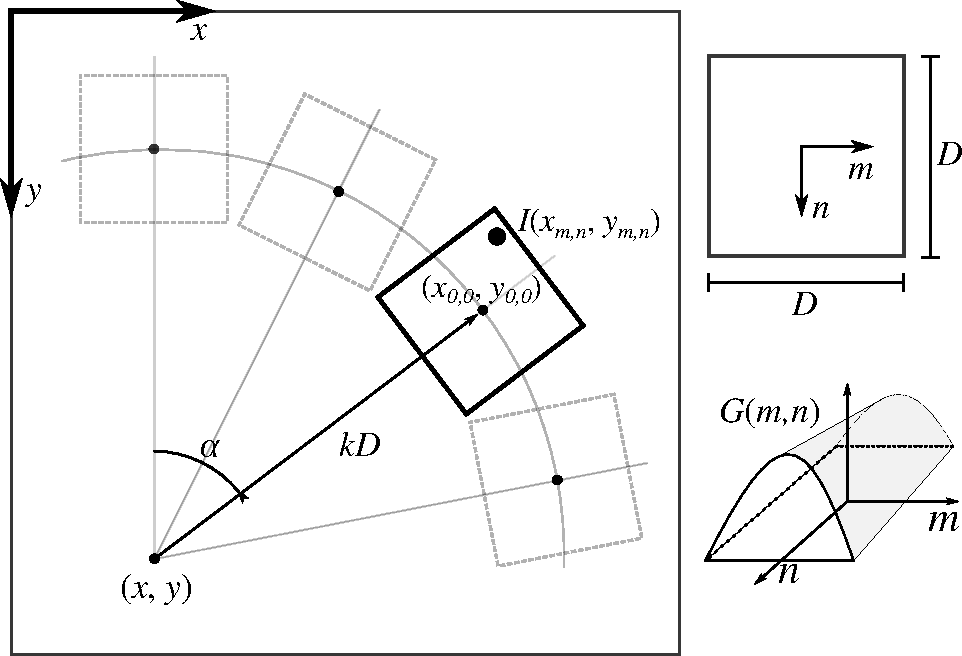
\includegraphics[width=0.5\columnwidth]{fig3}
	\caption{Geometry involved in the computation of the angular profile. In effect, the value of $p(x,y,\alpha,k,D)$ is the correlation of the image $I(x,y)$ with the kernel $G(m,n)$ of size $D\times D$ pixels, after rotating the kernel patch over angle $\alpha$ and shifting it over $kD$ with respect to $(x,y)$.}
	\label{fig3}
\end{figure}

Using the kernel we compute the local angular profile at any pixel location $(x,y)$ in the given image $I$ as:
\begin{equation}
p(x,y,\alpha,k,D)=\sum_{m}\sum_{n} I(x_{m,n},y_{m,n})\,G(m,n)
\label{eq:angularprofile}
\end{equation}
where the transformed image coordinates are obtained as:
\begin{equation}
\begin{bmatrix} x_{m,n} \\ y_{m,n} \end{bmatrix} =
\begin{bmatrix} x \\ y \end{bmatrix} +
kD\begin{bmatrix} \sin\alpha \\ -\!\cos\alpha \end{bmatrix} +
\begin{bmatrix} \cos\alpha & -\!\sin\alpha \\ \sin\alpha & \cos\alpha \end{bmatrix}
\begin{bmatrix} m \\ n \end{bmatrix}
\label{eq:xymn}
\end{equation}
and the summation is performed over all $(m,n)$ for which the kernel is defined. That is, $p(x,y,\alpha,k,D)$ is the correlation of the image with the kernel patch rotated over angle $\alpha$ and shifted over a distance $kD$ with respect to $(x,y)$ in the direction corresponding to that angle (Fig.~\ref{fig3}). In practice, $p$ is calculated for a discrete set of angles, $\alpha_{i}=i/(2\pi N_{\alpha}),\, i=0,\dots,N_{\alpha}-1$, where $N_{\alpha}$ is automatically set such that the circle with radius $kD$ is sampled with pixel resolution. The parameter $k$ is typically set slightly larger than 0.5 so as to scan the neighborhood around the considered pixel $(x,y)$. To obtain the image intensity at non-integer transformed locations $(x_{m,n},y_{m,n})$, linear interpolation is used.

In contrast with previous works, which used differential kernels for directional filtering and profiling \cite{yu1998rotated, can1999rapid, zhang2007automated}, we employ the matched kernel (Eq.~\ref{eq:G}), which avoids noise amplification. Although applying a set of rotated kernels is computationally more demanding than Hessian or steerable filtering based methods, it provides more geometrical flexibility in matching the kernels with the structures of interest while retaining excellent directional sensitivity. In our framework, the computational burden is drastically reduced by the foreground selection step, and further reduction is possible since the filtering process is highly parallelizable.

After computing the angular profile we further process it in order to extract several features (Fig.~\ref{fig4}) relevant for critical-point detection and characterization:

\paragraph{Peaks.} At each foreground pixel location we first determine how many and in which direction line-like image structures pass through it. This is done by finding the local maxima (``peaks'') in the angular profile at that location. Since the oriented kernels act as low-pass filters, the profile is sufficiently smooth to extract the peaks reliably using the iterative line searching algorithm \cite{flannery1992numerical}. The found peaks correspond to angles $\hat{\alpha}_{i}, i=1,\dots,N_{\hat{\alpha}}$, in which directions the image intensities are the highest. Here $N_{\hat{\alpha}}\leq 4$ to accommodate terminations, normal body points, and junctions (bifurcations and crossovers).

\paragraph{Likelihood.} For each $\hat{\alpha}_{i}$ we calculate a likelihood $l_i \in \left[ 0, 1 \right]  $ from the angular profile according to:
\begin{equation} 
l_i = \frac{p(x,y,\hat{\alpha}_{i},k,D)-p_{\min}}{p_{\max}-p_{\min}}
\end{equation}
where $p_{\min}$ and $p_{\max}$ denote, respectively, the minimum and maximum of $p(x,y,\alpha,k,D)$ over $\alpha$.

\paragraph{Energy.} Next we consider the local grid $\uppi_{i}(x,y,\hat{\alpha}_{i},k,D)$ for each $\hat{\alpha}_{i}$ (Fig.~\ref{fig4}), consisting of the transformed coordinates $(x_{m,n},y_{m,n})$ corresponding to $\alpha=\hat{\alpha}_{i}$ (Eq.~\ref{eq:xymn}), and we extract a refined centerline point set $\lambda_{i}$ (or ``streamline'') on this grid by finding for each $n$ the local maximum over $m$:
\begin{gather}
\label{eq:refine-centerline} 
\lambda_{i} = \left\{(x_{\hat{m}_{n},n},y_{\hat{m}_{n},n})\right\}_{n\,\in\,\left[-D/2,D/2\right]}\\[0.5ex]
\hat{m}_{n} = \argmax_{m\,\in\,\left[-D/2,D/2\right]} I(x_{m,n},y_{m,n})
\label{eq:hatm}
\end{gather}
We quantify how much the streamline deviates from a straight line by estimating its bending energy $u_{i}\geq0$ as:
\begin{equation}
u_{i} = \frac{1}{\Updelta m}\sum_{n} \left( \hat{m}_{n-1} - 2\hat{m}_{n} + \hat{m}_{n+1} \right)^2
\end{equation}
where $\Updelta m$ is the pixel spacing in the direction of $m$ and the summation extends over all $n$ for which the summand can be evaluated. This calculation is a discrete approximation of the integral squared second-order derivative of the centerline function if it were continuously defined.

\begin{figure}[!t]
	\centering
	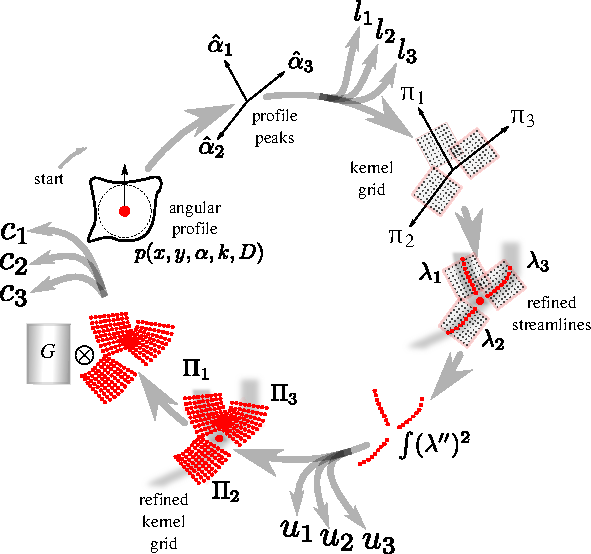
\includegraphics[width=0.5\columnwidth]{fig4}
	\caption{Flowchart of the feature extraction scheme. The example showcases a bifurcation but the same scheme is used also for terminations. The scheme, which starts with the angular profile $p(x,y,\alpha,k,D)$ and is executed clockwise, is applied to each pixel in the selected foreground regions and results in the set of features $l_i$, $u_i$, and $c_i$, where $i$ indexes the streamlines. See main text for details.}
	\label{fig4}
\end{figure}

\paragraph{Correlation.} Given a streamline $\lambda_{i}$ we estimate the orthogonal direction at each point in the set by averaging the orthogonal directions of the two neighboring streamline segments corresponding to that point (that is, from the point to the next point, and from the point to the previous point). Using these direction estimates we sample a refined local grid $\Uppi_{i}(x,y,\hat{\alpha}_{i},k,D)$, consisting of image coordinates $(\tilde{x}_{m,n},\tilde{y}_{m,n})$ relative to the streamline (Fig.~\ref{fig4}), and compute a normalized cross-correlation \cite{lewis1995fast} score $c_{i}\in[-1,1]$ as:
\begin{equation} 
\label{eq:correlation}
c_{i} = \frac{\sum_{m}\sum_{n} \bigl[I(\tilde{x}_{m,n},\tilde{y}_{m,n})-\bar{I}\bigr] \bigl[G(m,n)-\bar{G}\bigr]}{\sqrt{\sum_{m}\sum_{n}\bigl[I(\tilde{x}_{m,n},\tilde{y}_{m,n})-\bar{I}\bigr]^{2}\sum_{m}\sum_{n}\bigl[G(m,n)-\bar{G}\bigr]^{2}}}
\end{equation}
where, similar to the angular profile calculation (Eq.~\ref{eq:angularprofile}), the summations extend over all $(m,n)$ for which the kernel is defined, and $\bar{I}$ and $\bar{G}$ denote the mean of the image intensities and of the kernel values, respectively. Effectively $c_{i}$ quantifies the degree to which the template $G$ matches a straightened version of the streamline. To cover a range of possible scales (radii of the underlying image structures), we take the largest score of a set of templates with standard deviations of the Gaussian profile model \cite{su2012junction} covering $\left\lbrace 1,\dots,\left\lfloor{\frac{D}{2}}\right\rfloor\right\rbrace $ set of values measured in pixels.

\subsection{Fuzzy-Logic Based Mapping}
\label{subsec:flrb-detection}
The feature values extracted at each foreground image location subsequently need to be processed in order to assess the presence of a critical point and its type. Recognizing that in practice everything is ``a matter of degree'' \cite{zadeh1975fuzzy}, and allowing for nonlinear input-output mappings, we chose to use fuzzy logic for this purpose. Fuzzy logic has been successfully used in many areas of engineering \cite{mendel1995fuzzy} but to the best of our knowlege has not been explored for neuron critical-point analysis. We briefly describe the basics of fuzzy logic (Section~\ref{sec:FL}) and then present our specific fuzzy-logic system for calculating critical-point maps of neuron images (Section~\ref{sec:cp-detection}).
\begin{figure}
	\centering
	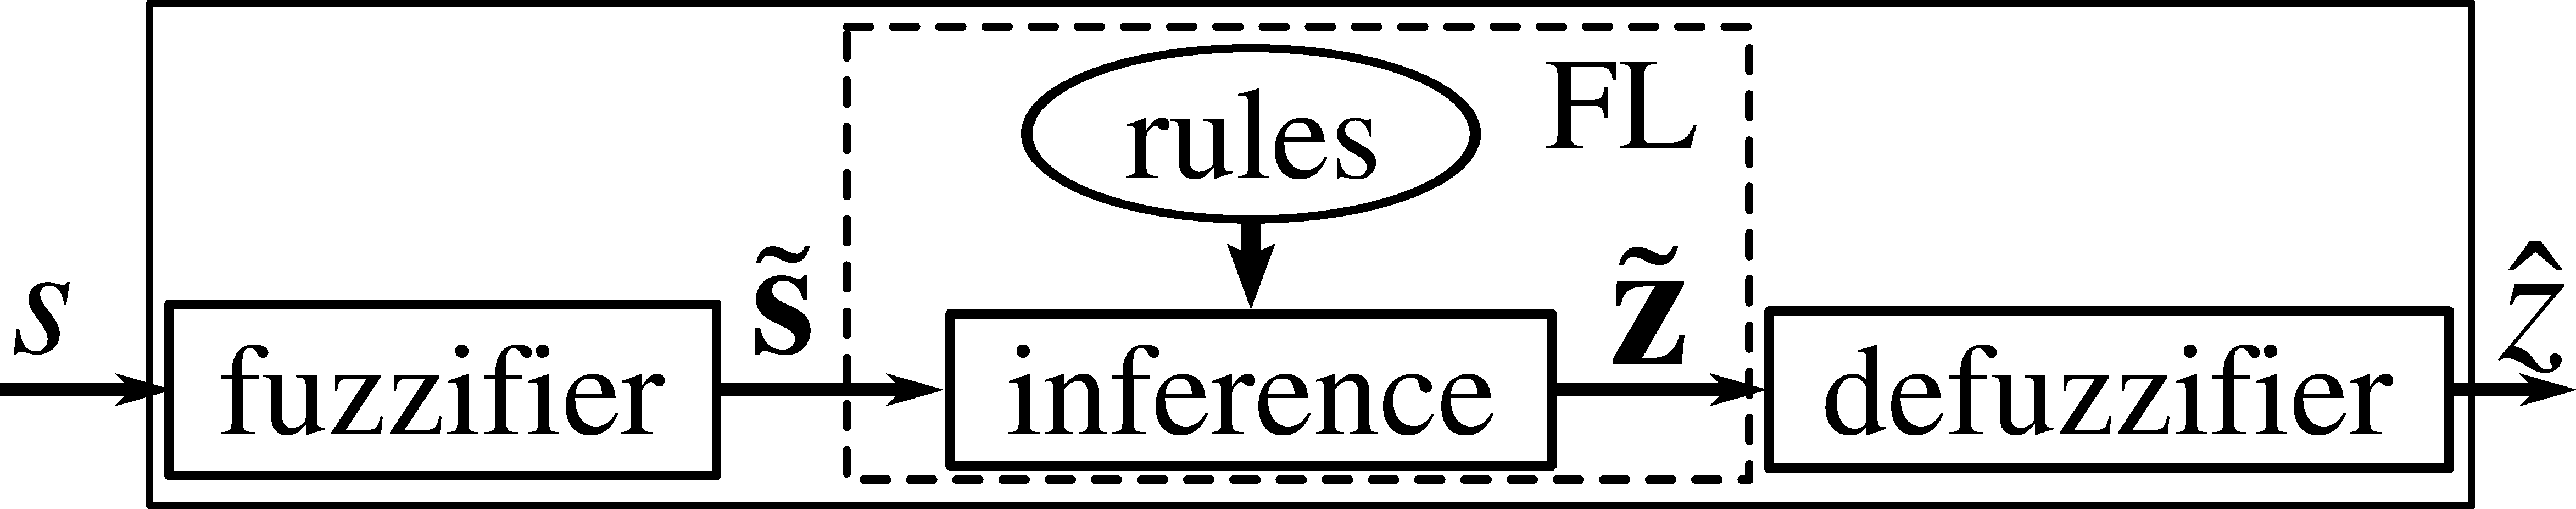
\includegraphics[width=0.5\columnwidth]{fig5}
	\caption{Scheme of a single input/output fuzzy-logic (FL) system. A scalar input value $s$ is converted to a vector $\tilde{\mathbf{s}}$ containing the memberships of $s$ for each of the input fuzzy sets, resulting in a vector $\tilde{\mathbf{z}}$ containing the memberships of $z$ for each of the output fuzzy sets.}
	\label{fig5}
\end{figure}
\subsubsection{Basics of Fuzzy Logic}
\label{sec:FL}
In a fuzzy-logic system (Fig.~\ref{fig5}), numerical inputs are first expressed in linguistic terms (the fuzzification step), and are then processed based on predefined rules to produce linguistic outputs (the inference step), which are finally turned back into numerical values (the defuzzification step).
\paragraph{Fuzzification.} Given an input scalar value $s\in\mathbb{R}$, the fuzzification step results in a vector $\tilde{\mathbf{s}}$ whose elements express the degree of membership of $s$  to input fuzzy sets, each corresponding to a linguistic term describing $s$. A fuzzy set is defined by a membership function $\mu:\mathbb{R}\rightarrow[0,1]$ quantifying the degree to which $s$ can be described by the corresponding linguistic term. Commonly used membership functions are trapezoidal, Gaussian, triangular, and piecewise linear \cite{mendel1995fuzzy}. As an example, we may have linguistic terms LOW and HIGH, representing the subjective notions ``low'' and ``high'', respectively. The degrees to which ``$s$ is low'' (which in this paper we will write as $s=\textrm{LOW}$) and ``$s$ is high'' ($s=\textrm{HIGH}$) are given by membership values $\mu_{\textrm{LOW}}(s)$ and $\mu_{\textrm{HIGH}}(s)$, respectively. The output of the fuzzification step thus becomes $\tilde{\mathbf{s}}=[\mu_{\textrm{LOW}}(s),\mu_{\textrm{HIGH}}(s)]^{T}$.
\paragraph{Inference.} The input fuzzy set memberships are processed by the inference engine to produce a fuzzy output based on rules expressing expert knowledge. The rules can be either explicitly defined or implicitly learned by some training process, and may express nonlinear input-output relationships and involve multiple inputs. In engineering applications, the rules are commonly given as IF-THEN statements about the input and output linguistic terms. For example, the output terms could be OFF, NONE, and ON, indicating whether a certain property of interest is ``off'', ``none'' (expressing ambiguity), or ``on''. A rule could then be:% \begin{split}\end{split} & \\ &
\begin{equation}
R_{i} \! : \ \  \textrm{IF} \  (s_{1}=\textrm{HIGH})\ \wedge\ (s_{2}=\textrm{LOW})\ \ \textrm{THEN}\ \ (z=\textrm{OFF})
\label{eq:rule-prototype}
\end{equation}
where $z\in\mathbb{R}$ is the variable over the output range. This is not a binary logical statement, where the input and output conditions can be only true or false, but a fuzzy logical statement, where the conditions are expressed in terms of memberships, in this case $\mu_{\textrm{HIGH}}(s_{1})$, $\mu_{\textrm{LOW}}(s_{2})$, and $\mu_{\textrm{OFF}}(z)$. Input conditions are often combined using the operators $\wedge$ (denoting fuzzy intersection) or $\vee$ (denoting fuzzy union), which are commonly defined as, respectively, the minimum and maximum of the arguments \cite{mendel1995fuzzy}. In our example, the IF-part of $R_{i}$ (Eq.~\ref{eq:rule-prototype}) would result in the following intermediate value (degree of verity):
\begin{equation}
\upsilon_{i} = \min\left\{\mu_{\textrm{HIGH}}(s_{1}),\mu_{\textrm{LOW}}(s_{2})\right\}
\end{equation}
This value is then used to constrain the fuzzy set corresponding to the output linguistic term addressed by $R_{i}$, in this case OFF, resulting in the output fuzzy set:
\begin{equation}
\Upsilon_{\!i}(z) = \min\left\{\mu_{\textrm{OFF}}(z),\upsilon_{i}\right\}
\end{equation}
In practice there may be many rules $R_{i}, i=1,\dots,N_{R}$, which are aggregated by the inference engine to produce a single output fuzzy set $\Upsilon$. The common way to do this \cite{mendel1995fuzzy} is by means of a weighted fuzzy union:
\begin{equation}
\Upsilon(z) = \max\left\{w_{1}\Upsilon_{\!1}(z),\dots,w_{N_{R}}\Upsilon_{\!N_{R}}(z)\right\}
\end{equation}
Although it is possible to assign a different weight to each rule by setting $w_{i}\in[0,1]$, in our applications this is not critical, and therefore we simply use $w_{i}=1$ for all $i$.

\paragraph{Defuzzification.} In the final step of the fuzzy-logic system, the fuzzy output $\Upsilon$ is converted back to a scalar output value. Although there are many ways to do this, a common choice is to calculate the centroid \cite{mendel1995fuzzy}:
\begin{equation}
\label{eq:centroid-general}
\hat{z} = \frac{\int z\Upsilon(z)dz}{\int\Upsilon(z)dz} 
\end{equation}
With this value we can finally calculate the vector of output fuzzy set memberships: $\tilde{\mathbf{z}}=[\mu_{\textrm{OFF}}(\hat{z}),\mu_{\textrm{NONE}}(\hat{z}),\mu_{\textrm{ON}}(\hat{z})]^{T}$.

\begin{figure}[!t]
	\centering
	\begin{tabular}{c@{\hspace{1em}}c@{\hspace{1em}}}
	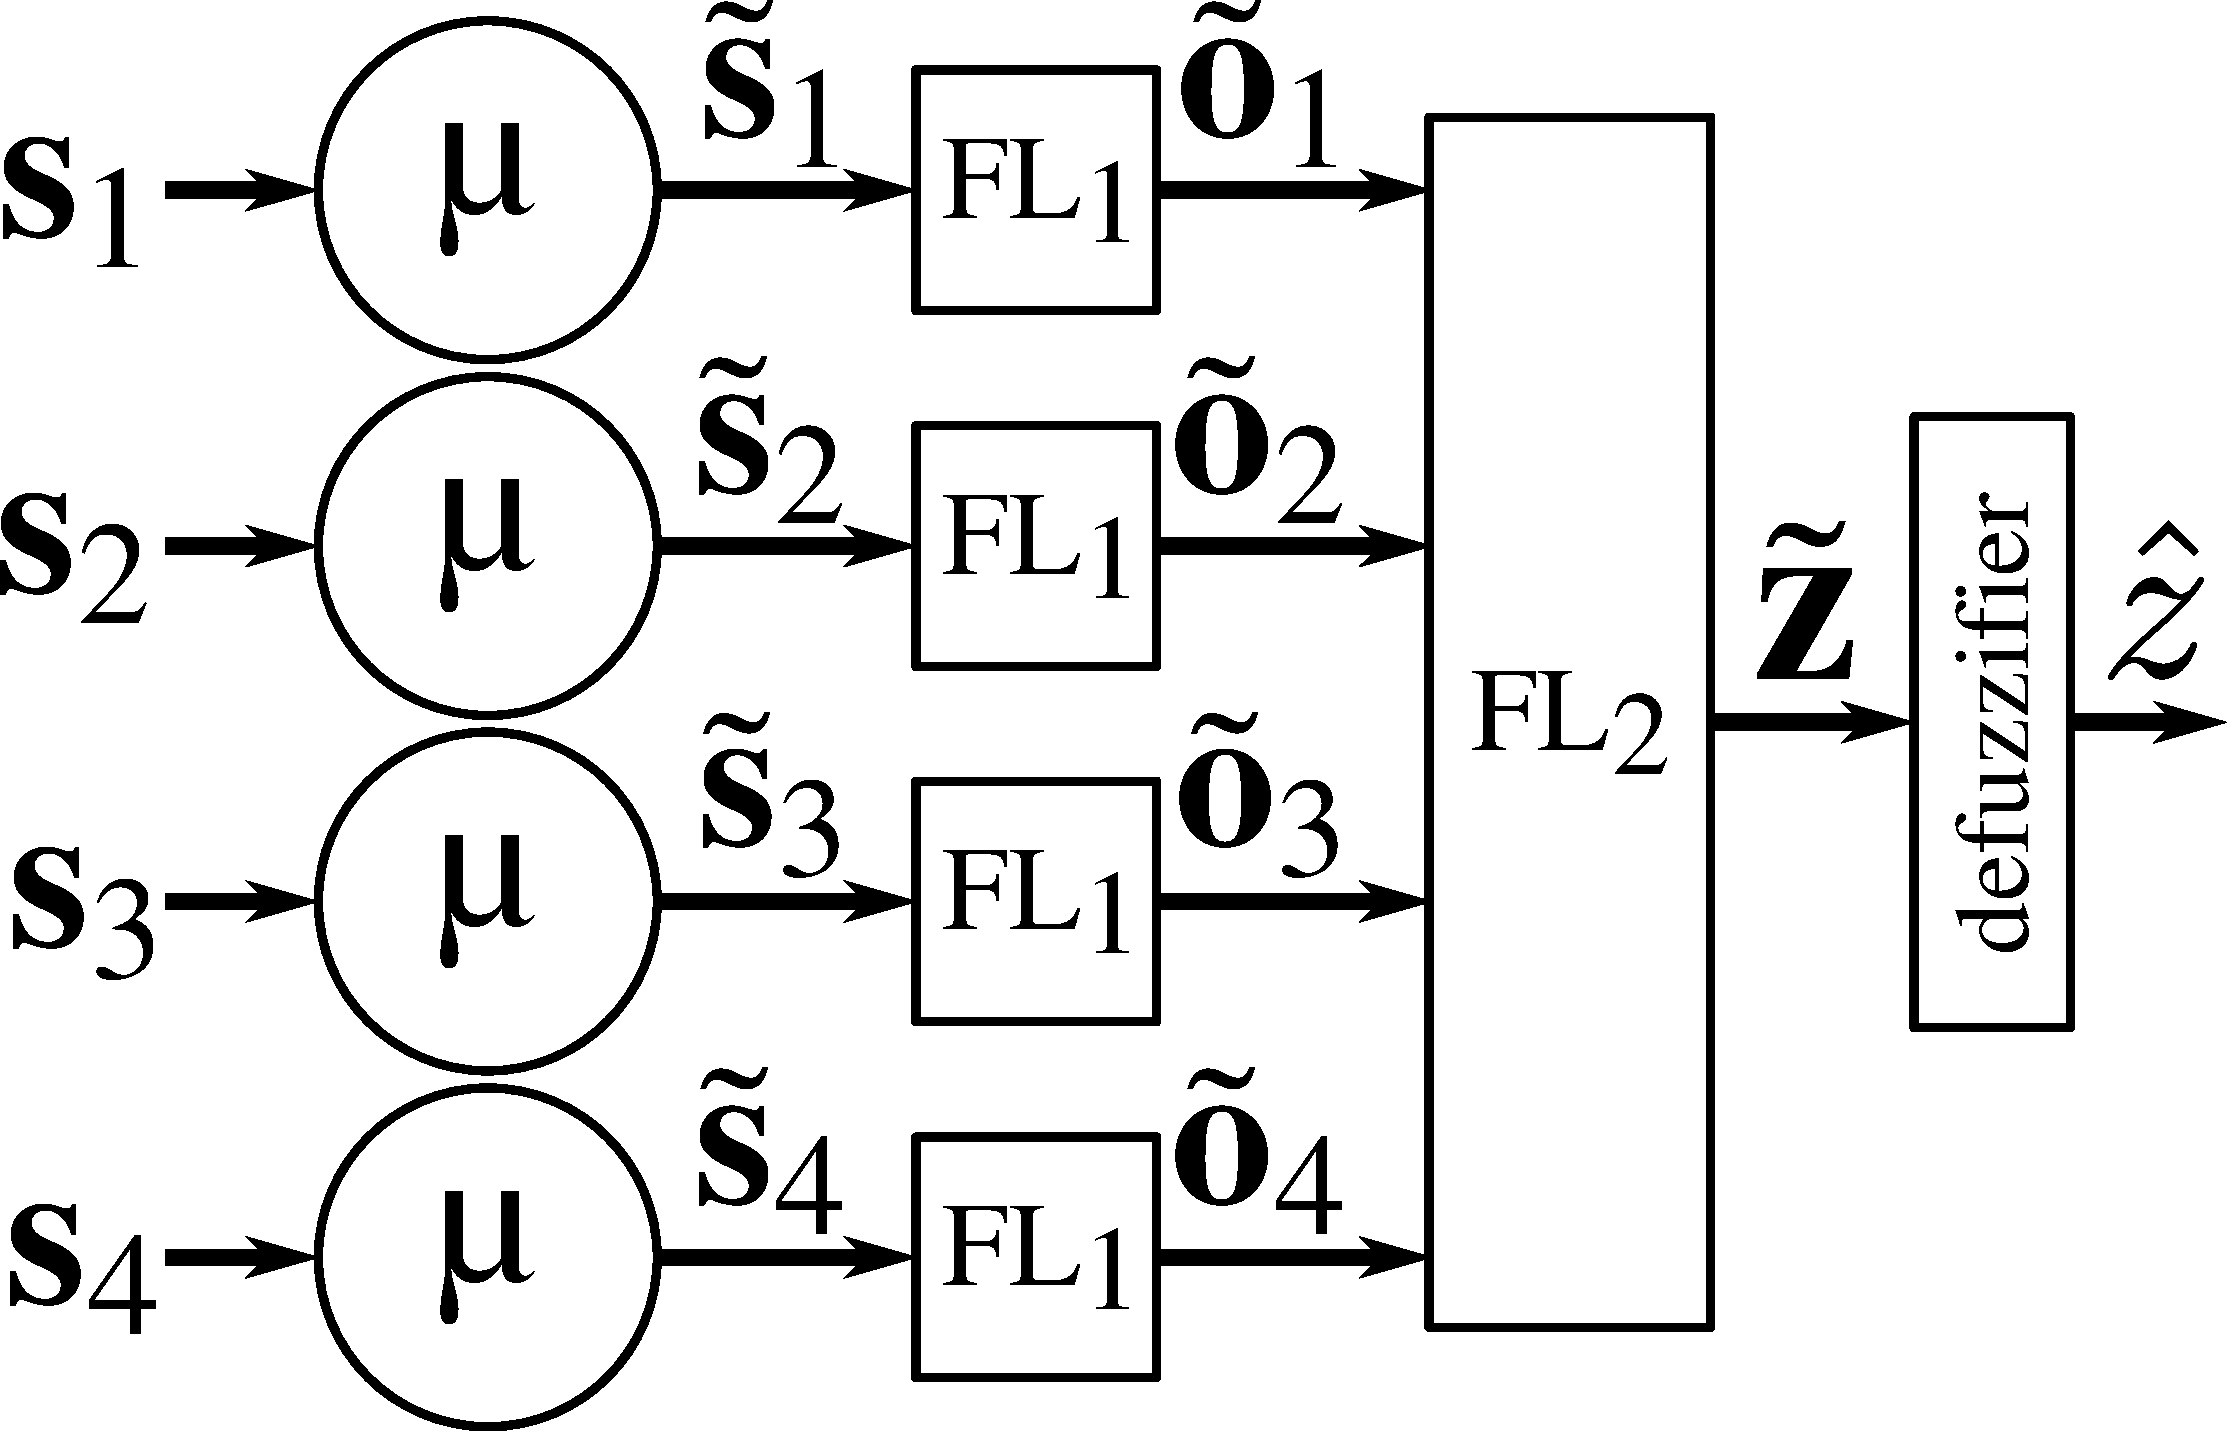
\includegraphics[height=0.27\columnwidth]{fig6a} &
	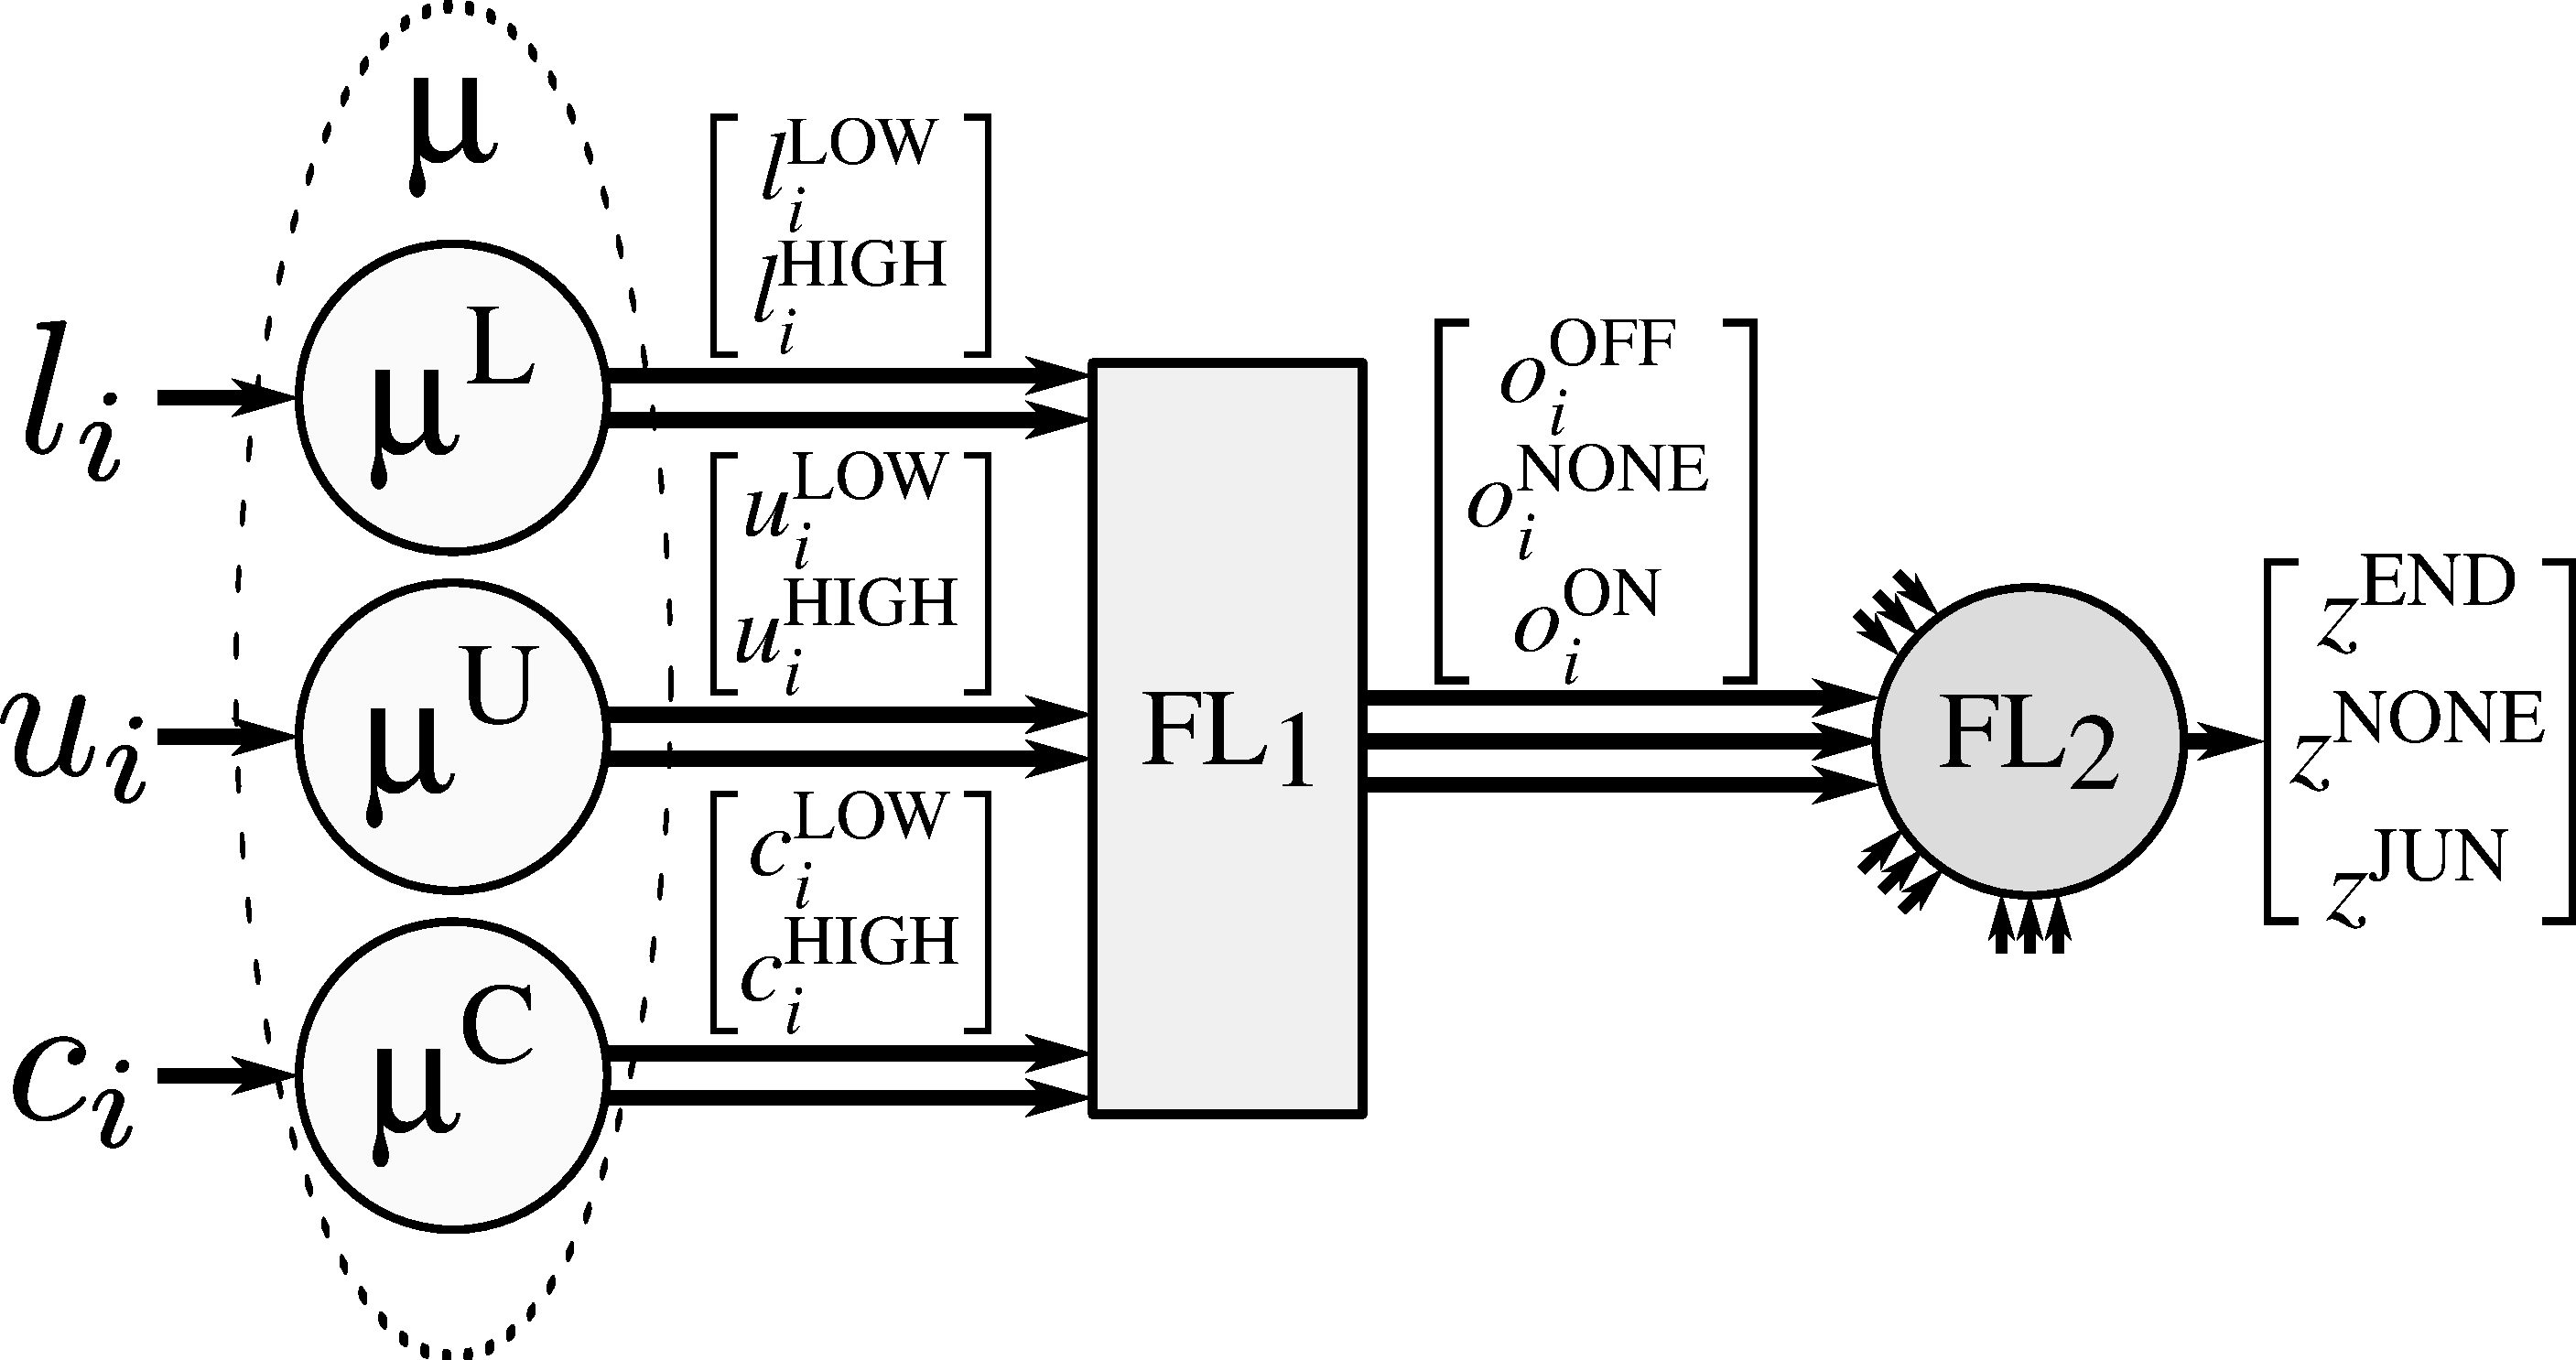
\includegraphics[height=0.27\columnwidth]{fig6b} \\
	a) & b) 
	\end{tabular}
	\caption{Architecture of the proposed fuzzy-logic system: a) critical-point detection: a cascade of two fuzzy-logic modules ($\textrm{FL}_{1}$ and $\textrm{FL}_{2}$), where the first determines the degree to which streamlines (up to four) are present at the image location under consideration, and based on this information the second determines the degree to which that location corresponds to the possible types of critical points, b) processing the information of one streamline. Input feature values are fuzzified into linguistic terms LOW and HIGH, which are translated by the first fuzzy-logic module ($\textrm{FL}_{1}$) into intermediate linguistic terms OFF, NONE, ON, which are finally translated by the second fuzzy-logic module ($\textrm{FL}_{2}$) into linguistic terms END, NONE, JUN.}
	\label{fig6}
\end{figure}

\subsubsection{Termination and Junction Mapping}
\label{sec:cp-detection}
To determine the presence and type of critical point at any foreground image location, we use a cascade of two fuzzy-logic systems, representing two decision levels (Fig.~\ref{fig6}a). The first level takes as input vectors $\mathbf{s}_{i}=[l_{i},u_{i},c_{i}]$, $i=1,\dots,4$, which contain the features for each of the streamlines extracted in the angular profile analysis step at the image location under consideration (Section~\ref{subsubsec:angular-profile}). For each streamline (Fig.~\ref{fig6}b), the features are fuzzified ($\mu$) and processed by the first fuzzy-logic module ($\textrm{FL}_{1}$), which determines the degree to which the streamline indeed represents a line-like image structure (ON), or not (OFF), or whether the image structure is ambiguous (NONE). In cases where less than four streamlines were found by the angular profile analysis step, the feature vectors of the nonexisting streamlines are set to $\mathbf{0}$. The fuzzy output for all four streamlines together forms the input for the second decision level, where another fuzzy-logic module ($\textrm{FL}_{2}$) determines the degree to which the image location corresponds to a junction (JUN), or a termination (END), or neither of these (NONE).

The input streamline features, $l_{i}$, $u_{i}$, $c_{i}$, are expressed in linguistic terms LOW and HIGH using membership functions $\mu_{\textrm{LOW}}$ and $\mu_{\textrm{HIGH}}$ defined for each type of feature. In our application we use trapezoidal membership functions, each having two inflection points, such that $\mu_{\textrm{LOW}}$ and $\mu_{\textrm{HIGH}}$ are each other's complement (Fig.~\ref{fig7}). For example, the degrees to which $l_{i}=\textrm{LOW}$ and $l_{i}=\textrm{HIGH}$, are given by $l_{i}^{\textrm{LOW}}=\mu^{L}_{\textrm{LOW}}(l_{i})$ and $l_{i}^{\textrm{HIGH}}=\mu^{L}_{\textrm{HIGH}}(l_{i})=1-l_{i}^{\textrm{LOW}}$, respectively, and because of this complementarity we often simply write $\mu^{L}$ to refer to both membership functions (Fig.~\ref{fig6}). Similarly, the membership degrees of $u_{i}$ and $c_{i}$ are given by $\mu^{U}$ and $\mu^{C}$, respectively. Summarizing, we use the following notations and definitions for the fuzzification step:
\begin{equation}
\begin{array}{lcccl}
\mu^{L}\!:\ & l_{i} & \rightarrow & \tilde{\mathbf{l}}_{i} & = \left[l_{i}^{\textrm{LOW}}\!,\, l_{i}^{\textrm{HIGH}}\right]^T \\[1ex]
\mu^{U}\!:\ & u_{i} & \rightarrow & \tilde{\mathbf{u}}_{i} & = \left[u_{i}^{\textrm{LOW}}\!,\, u_{i}^{\textrm{HIGH}}\right]^T \\[1ex]
\mu^{C}\!:\ & c_{i} & \rightarrow & \tilde{\mathbf{c}}_{i} & = \left[c_{i}^{\textrm{LOW}}\!,\, c_{i}^{\textrm{HIGH}}\right]^T
\end{array}
\end{equation}
and the lower and higher inflection points of $\mu^{L}$ are denoted by $L_{\textrm{LOW}}$ and $L_{\textrm{HIGH}}$, and similarly $U_{\textrm{LOW}}$ and $U_{\textrm{HIGH}}$ for $\mu^{U}$, and $C_{\textrm{LOW}}$ and $C_{\textrm{HIGH}}$ for $\mu^{C}$ (Fig.~\ref{fig7}).

\begin{figure}%[!t]
	\centering
	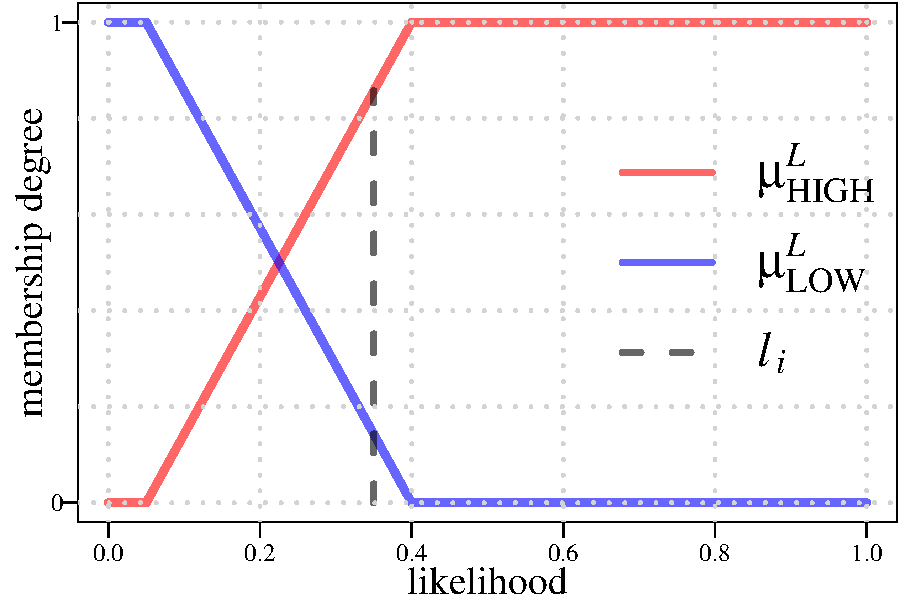
\includegraphics[height=9em]{L_fuzzification_1}
	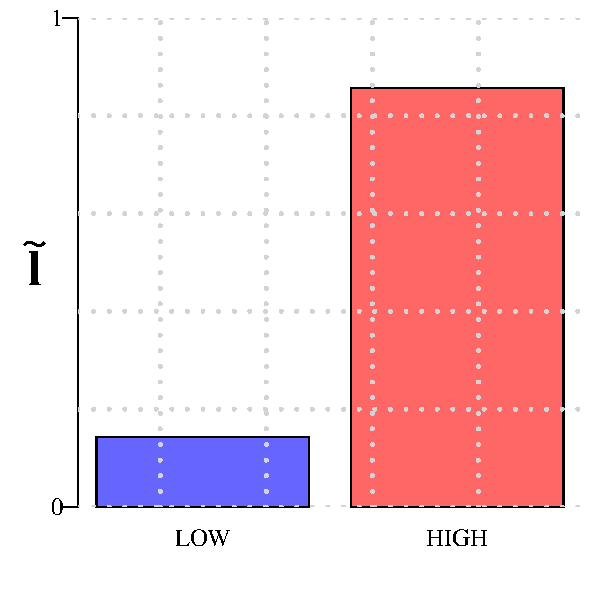
\includegraphics[height=9em]{L_fuzzification_2} \\[2ex]
	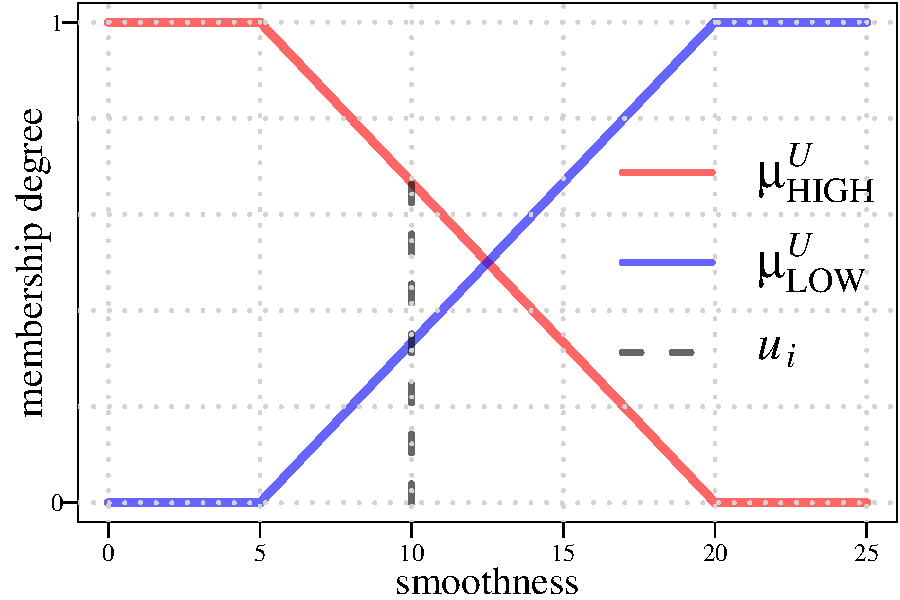
\includegraphics[height=9em]{U_fuzzification_1}
	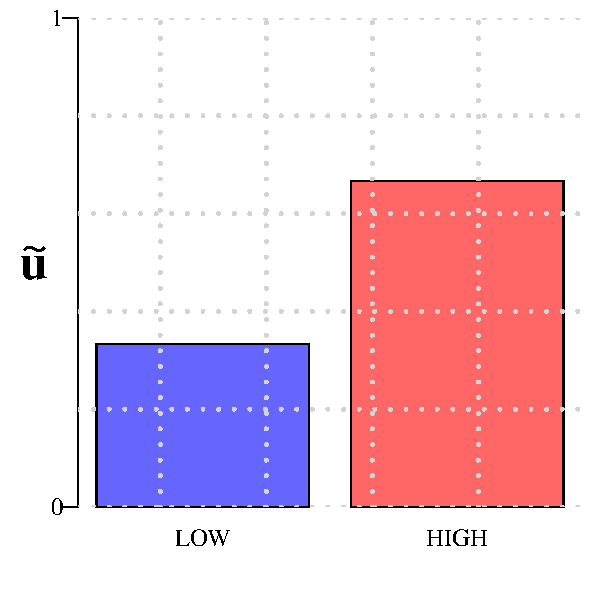
\includegraphics[height=9em]{U_fuzzification_2} \\[2ex]
	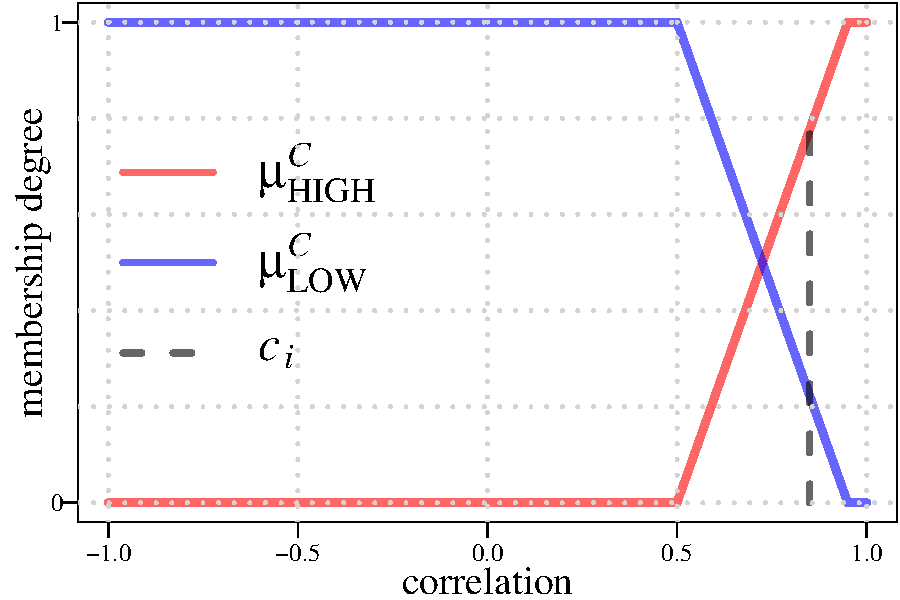
\includegraphics[height=9em]{C_fuzzification_1}
	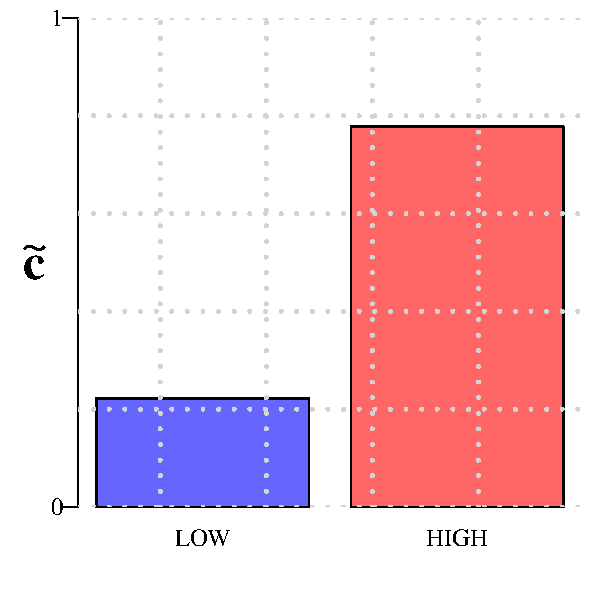
\includegraphics[height=9em]{C_fuzzification_2} \\
	\caption{Input membership functions used in the fuzzification step for $\textrm{FL}_{1}$. Example LOW and HIGH membership values are shown (right column) for input values (dashed vertical lines in the plots on the left) $l_{i}=0.35$ (top row), $u_{i}=10$ (middle row), and $c_{i}=0.85$ (bottom row). The inflection points of the membership functions are, respectively, $L_{\textrm{LOW}}=0.05$ and $L_{\textrm{HIGH}}=0.4$ for $\mu^{L}$, $U_{\textrm{HIGH}}=5$ and $U_{\textrm{LOW}}=20$ for $\mu^{U}$, and $C_{\textrm{LOW}}=0.5$ and $C_{\textrm{HIGH}}=0.95$ for $\mu^{C}$. Notice that features $u_{i}$ (the centerline bending energies of the streamlines) are reinterpreted here to express the degree of smoothness (hence the inverted membership functions as compared to the other two).}
	\label{fig7}
\end{figure}
Taken together, the input to $\textrm{FL}_{1}$ is the matrix of memberships $\tilde{\mathbf{s}}_{i}=[\tilde{\mathbf{l}}_{i},\tilde{\mathbf{u}}_{i},\tilde{\mathbf{c}}_{i}]$, and the output is the vector $\tilde{\mathbf{o}}_{i}$ of memberships to the linguistic terms OFF, NONE, ON:
\begin{equation}
\mathrm{FL}_{1}\!:\ \tilde{\mathbf{s}}_{i} \rightarrow \tilde{\mathbf{o}}_{i} = \left[o_{i}^{\textrm{OFF}}\!,\, o_{i}^{\textrm{NONE}}\!,\, o_{i}^{\textrm{ON}}\right]^T
\label{eq:FL1}
\end{equation}
To calculate these memberships, scalar variable $o$ is introduced, where $o=0$ corresponds to OFF, $o=1$ to NONE, and $o=2$ to ON. Also, Gaussian membership functions $\mu_{\textrm{OFF}}^{O}$, $\mu_{\textrm{NONE}}^{O}$ and $\mu_{\textrm{ON}}^{O}$  are defined, centered around $0$, $1$, and $2$, respectively (Fig.~\ref{fig9}), and with fixed standard deviation $0.4$ so that they sum to about 1 in the interval $[0,2]$. The rules used by $\textrm{FL}_{1}$ to associate the input terms LOW and HIGH to the output terms OFF, NONE, and ON, are given in Table~\ref{tab:rules-FL1}. They are based on the heuristic assumption that a line-like image structure exists (ON) if the evidence represented by all three features support it (HIGH). By contrast, if the likelihood is LOW and at least one other feature is also LOW, this indicates that no such structure exists (OFF). In all remaining cases, some structure may exist, but it is not line-like (NONE). As an example, rule $R_8$ (Table~\ref{tab:rules-FL1}) is given by:
\begin{equation}
R_8\!:\ \ \textrm{IF}\ (l=\textrm{HIGH})\ \wedge\ (u=\textrm{HIGH})\ \wedge\ (c=\textrm{HIGH}) \textrm{THEN}\ (o = \textrm{ON})
\end{equation}
which results in the verity value:
\begin{equation}
\upsilon_{8} = \min\left\{\mu_{\textrm{HIGH}}^{L}(l), \mu_{\textrm{HIGH}}^{U}(u), \mu_{\textrm{HIGH}}^{C}(c)\right\}
\end{equation}
and the output fuzzy set: 
\begin{equation}
\Upsilon_{8}(o) = \min\left\{\mu_{\textrm{ON}}^{O}(o),\upsilon_{8}\right\}
\end{equation}
All the rules are resolved and combined as:
\begin{equation}
\Upsilon(o) = \max\left\{\Upsilon_{1}(o),\dots,\Upsilon_{8}(o)\right\}
\end{equation}
and centroid defuzzification then results in a scalar output value $\hat{o}$. This procedure is repeated for each streamline, yielding $\hat{o}_{i}, i=1,\dots,4$, from which the output of each $\mathrm{FL}_{1}$ (Eq.~\ref{eq:FL1}) is calculated using the membership functions:
\begin{equation}
\tilde{\mathbf{o}}_{i} = \left[\mu_{\textrm{OFF}}^{O}(\hat{o}_{i}),\, \mu_{\textrm{NONE}}^{O}(\hat{o}_{i}),\, \mu_{\textrm{ON}}^{O}(\hat{o}_{i})\right]^{T}
\end{equation}

\begin{figure}
	\centering
	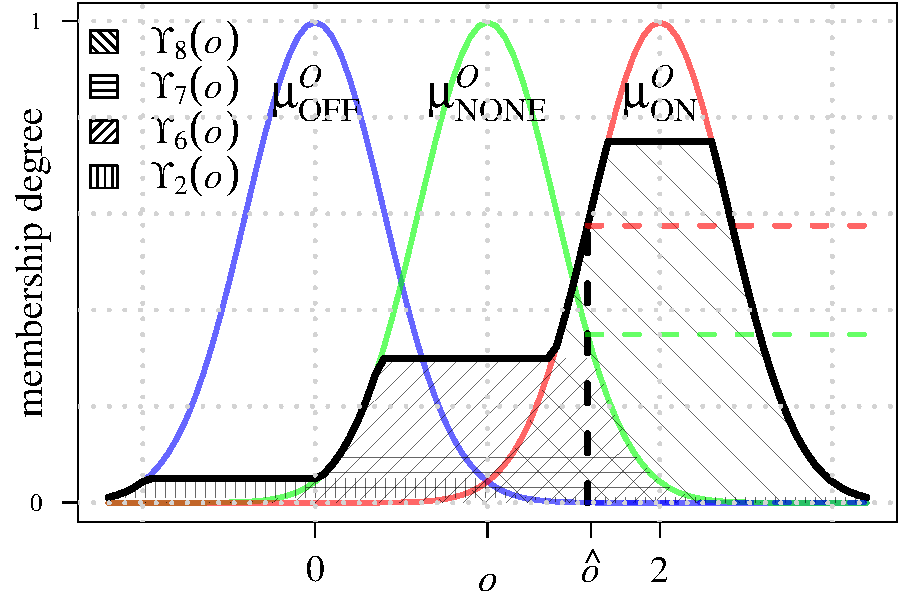
\includegraphics[height=9em]{fig9a}
	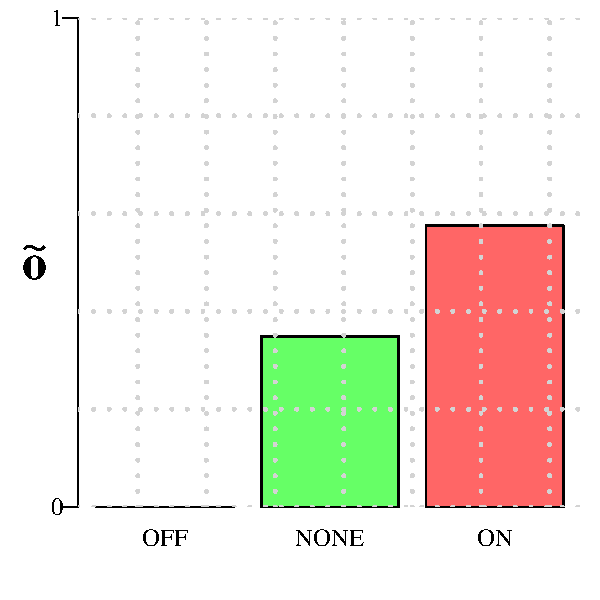
\includegraphics[height=9em]{fig9b}
	\caption{Output membership functions used in module $\mathrm{FL}_{1}$. Example output fuzzy sets $\Upsilon_{\!i}$ corresponding to rules $R_i$ from Table~\ref{tab:rules-FL1} are shown as the textured areas. Value $\hat{o}$ (left panel) represents the centroid of the aggregated output fuzzy sets. The resulting output membership values (right panel) serve as input for module $\mathrm{FL}_{2}$.}
	\label{fig9}
\end{figure}

\begin{table}[!t]
	\caption{The set of rules employed by $\mathrm{FL}_{1}$.}
	\label{tab:rules-FL1}
	\centering
	\begin{tabular}{c | c c c | c }
		$R_{i}$ & $l$ & $u$ & $c$ & $o$ \\
		\hline
		1 & LOW  & LOW  & LOW  & OFF \\
		2 & LOW  & LOW  & HIGH & OFF \\
		3 & LOW  & HIGH & LOW  & OFF \\
		\hline
		4 & LOW  & HIGH & HIGH  & NONE \\ 
		5 & HIGH & LOW  & LOW   & NONE \\ 
		6 & HIGH & LOW  & HIGH  & NONE \\ 
		7 & HIGH & HIGH & LOW   & NONE \\ 
		\hline
		8 & HIGH & HIGH & HIGH  & ON \\ 
	\end{tabular}
\end{table}

\begin{table}[!t]
	\caption{The set of rules employed by $\mathrm{FL}_{2}$. Empty entries indicate ``don't care'' (could be OFF, NONE, or ON).}
	\label{tab:rules-FL2}
	\centering
	\begin{tabular}{c | c c c c | c }
		$R_{i}$ & $o_{1}$   & $o_{2}$   & $o_{3}$   & $o_{4}$  & $z$ \\
		\hline
		1 & OFF  & OFF  & OFF  & OFF & NONE \\
		2 & OFF  & OFF  & OFF  & ON  & END  \\
		3 & OFF  & OFF  & ON   & OFF & END  \\
		4 & OFF  & OFF  & ON   & ON  & NONE \\
		\hline
		5 & OFF  & ON   & OFF  & OFF & END  \\
		6 & OFF  & ON   & OFF  & ON  & NONE \\
		7 & OFF  & ON   & ON   & OFF & NONE \\
		8 & OFF  & ON   & ON   & ON  & JUN  \\
		\hline
		9 & ON   & OFF  & OFF  & OFF & END  \\
		10&ON   & OFF  & OFF  & ON  & NONE  \\
		11&ON   & OFF  & ON   & OFF & NONE  \\
		12&ON   & OFF  & ON   & ON  & JUN  \\
		\hline
		13&ON   & ON   & OFF  & OFF & NONE  \\
		14&ON   & ON   & OFF  & ON  & JUN  \\
		15&ON   & ON   & ON   & OFF & JUN  \\
		16&ON   & ON   & ON   & ON  & JUN  \\
		\hline
		17&NONE & NONE &      &      & NONE \\
		18&NONE &      & NONE &      & NONE \\
		19&NONE &      &      & NONE & NONE \\
		20&     & NONE & NONE &      & NONE \\
		21&     & NONE &      & NONE & NONE \\
		22&     &      & NONE & NONE & NONE \\     
	\end{tabular}
\end{table}

Moving on to the next level, the input to $\mathrm{FL}_{2}$ is the matrix of memberships $\tilde{\mathbf{o}}=\left[\tilde{\mathbf{o}}_{1},\tilde{\mathbf{o}}_{2},\tilde{\mathbf{o}}_{3},\tilde{\mathbf{o}}_{4}\right]$, and the output is the vector $\tilde{\mathbf{z}}$ of memberships to the linguistic terms END (termination), NONE (no critical point), JUN (junction):
\begin{equation}
\mathrm{FL}_{2}\!:\ \tilde{\mathbf{o}} \rightarrow \tilde{\mathbf{z}} = \left[z^{\textrm{END}}\!,\, z^{\textrm{NONE}}\!,\, z^{\textrm{JUN}}\right]^T
\label{eq:FL2}
\end{equation}
To calculate these memberships we introduce scalar variable $z$, where $z=1$ corresponds to END, $z=2$ to NONE, and $z=3$ to JUN, and we define corresponding Gaussian membership functions $\mu_{\textrm{END}}^{Z}$, $\mu_{\textrm{NONE}}^{Z}$, and $\mu_{\textrm{JUN}}^{Z}$, centered around $1$, $2$, and $3$, respectively, and with fixed standard deviation $0.4$ as before (Fig.~\ref{fig10}). The rules used by $\mathrm{FL}_{2}$ to associate the input terms OFF, NONE, ON to the output terms END, NONE, JUN are given in Table~\ref{tab:rules-FL2}. They are based on the heuristic assumption that there is a termination (END) if a single streamline is confirmed to correspond to a line-like image structure (ON) and the other three are confirmed to not correspond to such a structure (OFF). Conversely, if at least three are ON, there must be a junction at that location. Finally, if two are ON and two are OFF, or if at least two streamlines are ambiguous (NONE), we assume there is no critical point. Similar to $\mathrm{FL}_{1}$, all the rules of $\mathrm{FL}_{2}$ are evaluated and their results combined as:
\begin{equation}
\Upsilon(z) = \max\left\{\Upsilon_{1}(z),\dots,\Upsilon_{22}(z)\right\}
\end{equation}
which, after centroid defuzzification, results in a scalar output value $\hat{z}$, from which the output of $\mathrm{FL}_{2}$ (Eq.~\ref{eq:FL2}) is calculated using the membership functions:
\begin{equation}
\tilde{\mathbf{z}} = \left[\mu_{\textrm{END}}^{Z}(\hat{z}),\, \mu_{\textrm{NONE}}^{Z}(\hat{z}),\, \mu_{\textrm{JUN}}^{Z}(\hat{z})\right]^{T}
\end{equation}
The proposed fuzzy-logic system is applied to each foreground pixel location $(x,y)\in F$ (Section~\ref{subsubsec:foreground-selection}) so that all memberships introduced above may be indexed by $(x,y)$. Based on this, the following two maps are calculated:
\begin{equation}
I_{\textrm{END}}(x,y)=\left\{
\begin{array}{l@{\qquad}l}
z^{\textrm{END}}(x,y) & \textrm{if}\ (x,y)\in F \\
0 & \textrm{otherwise}
\end{array}
\right.
\end{equation}
\begin{equation}
I_{\textrm{JUN}}(x,y)=\left\{
\begin{array}{l@{\qquad}l}
z^{\textrm{JUN}}(x,y) & \textrm{if}\ (x,y)\in F \\
0 & \textrm{otherwise}
\end{array}
\right.
\end{equation}
which indicate the degree to which any pixel $(x,y)$ belongs to a termination or a junction, respectively.
\begin{figure}[ht!]
	\centering
	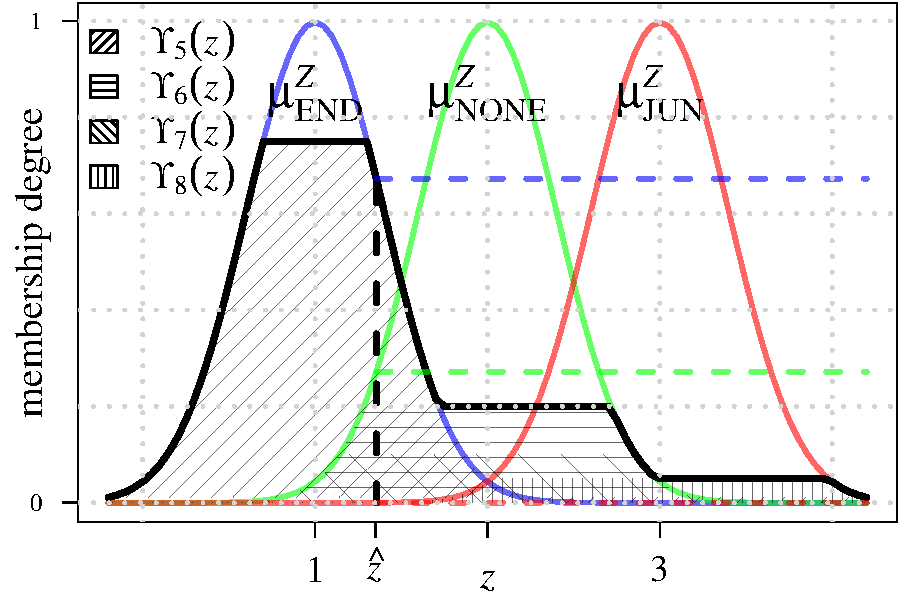
\includegraphics[height=9em]{fig10a}
	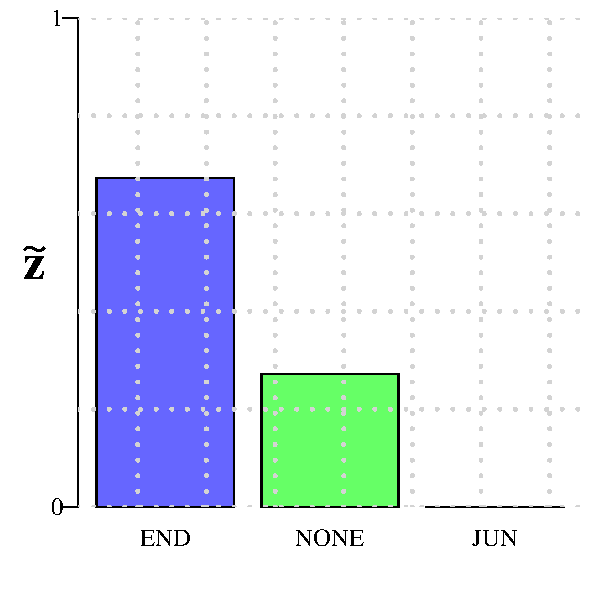
\includegraphics[height=9em]{fig10b}
	\caption{Output membership functions used in module $\mathrm{FL}_{2}$. Example output fuzzy sets $\Upsilon_{\!i}$ corresponding to rules $R_i$ from Table~\ref{tab:rules-FL2} are shown as the textured areas. Value $\hat{z}$ (left panel) represents the centroid of the aggregated output fuzzy sets. The resulting output membership values (right panel) indicate the degree to which there may be a termination (END), junction (JUN), or neither of these (NONE) at the image pixel location under consideration.}
	\label{fig10}
\end{figure}
\subsection{Critical-Point Determination}
\label{sec:CPextraction}
The ultimate aim of the introduced method is to provide a list of critical points in the neuron image, with each point fully characterized in terms of type, location, size, and main branch direction(s). Since each critical point of a neuronal tree typically covers multiple neighboring pixels in the image, giving rise to a high value at the corresponding pixels in the maps $I_{\textrm{END}}$ and $I_{\textrm{JUN}}$, the final task is to segment the maps and to aggregate the information within each segmented region.
\begin{figure}[!b]
	\centering
	\begin{tabular}{c@{\hspace{2em}}c@{\hspace{2em}}}
	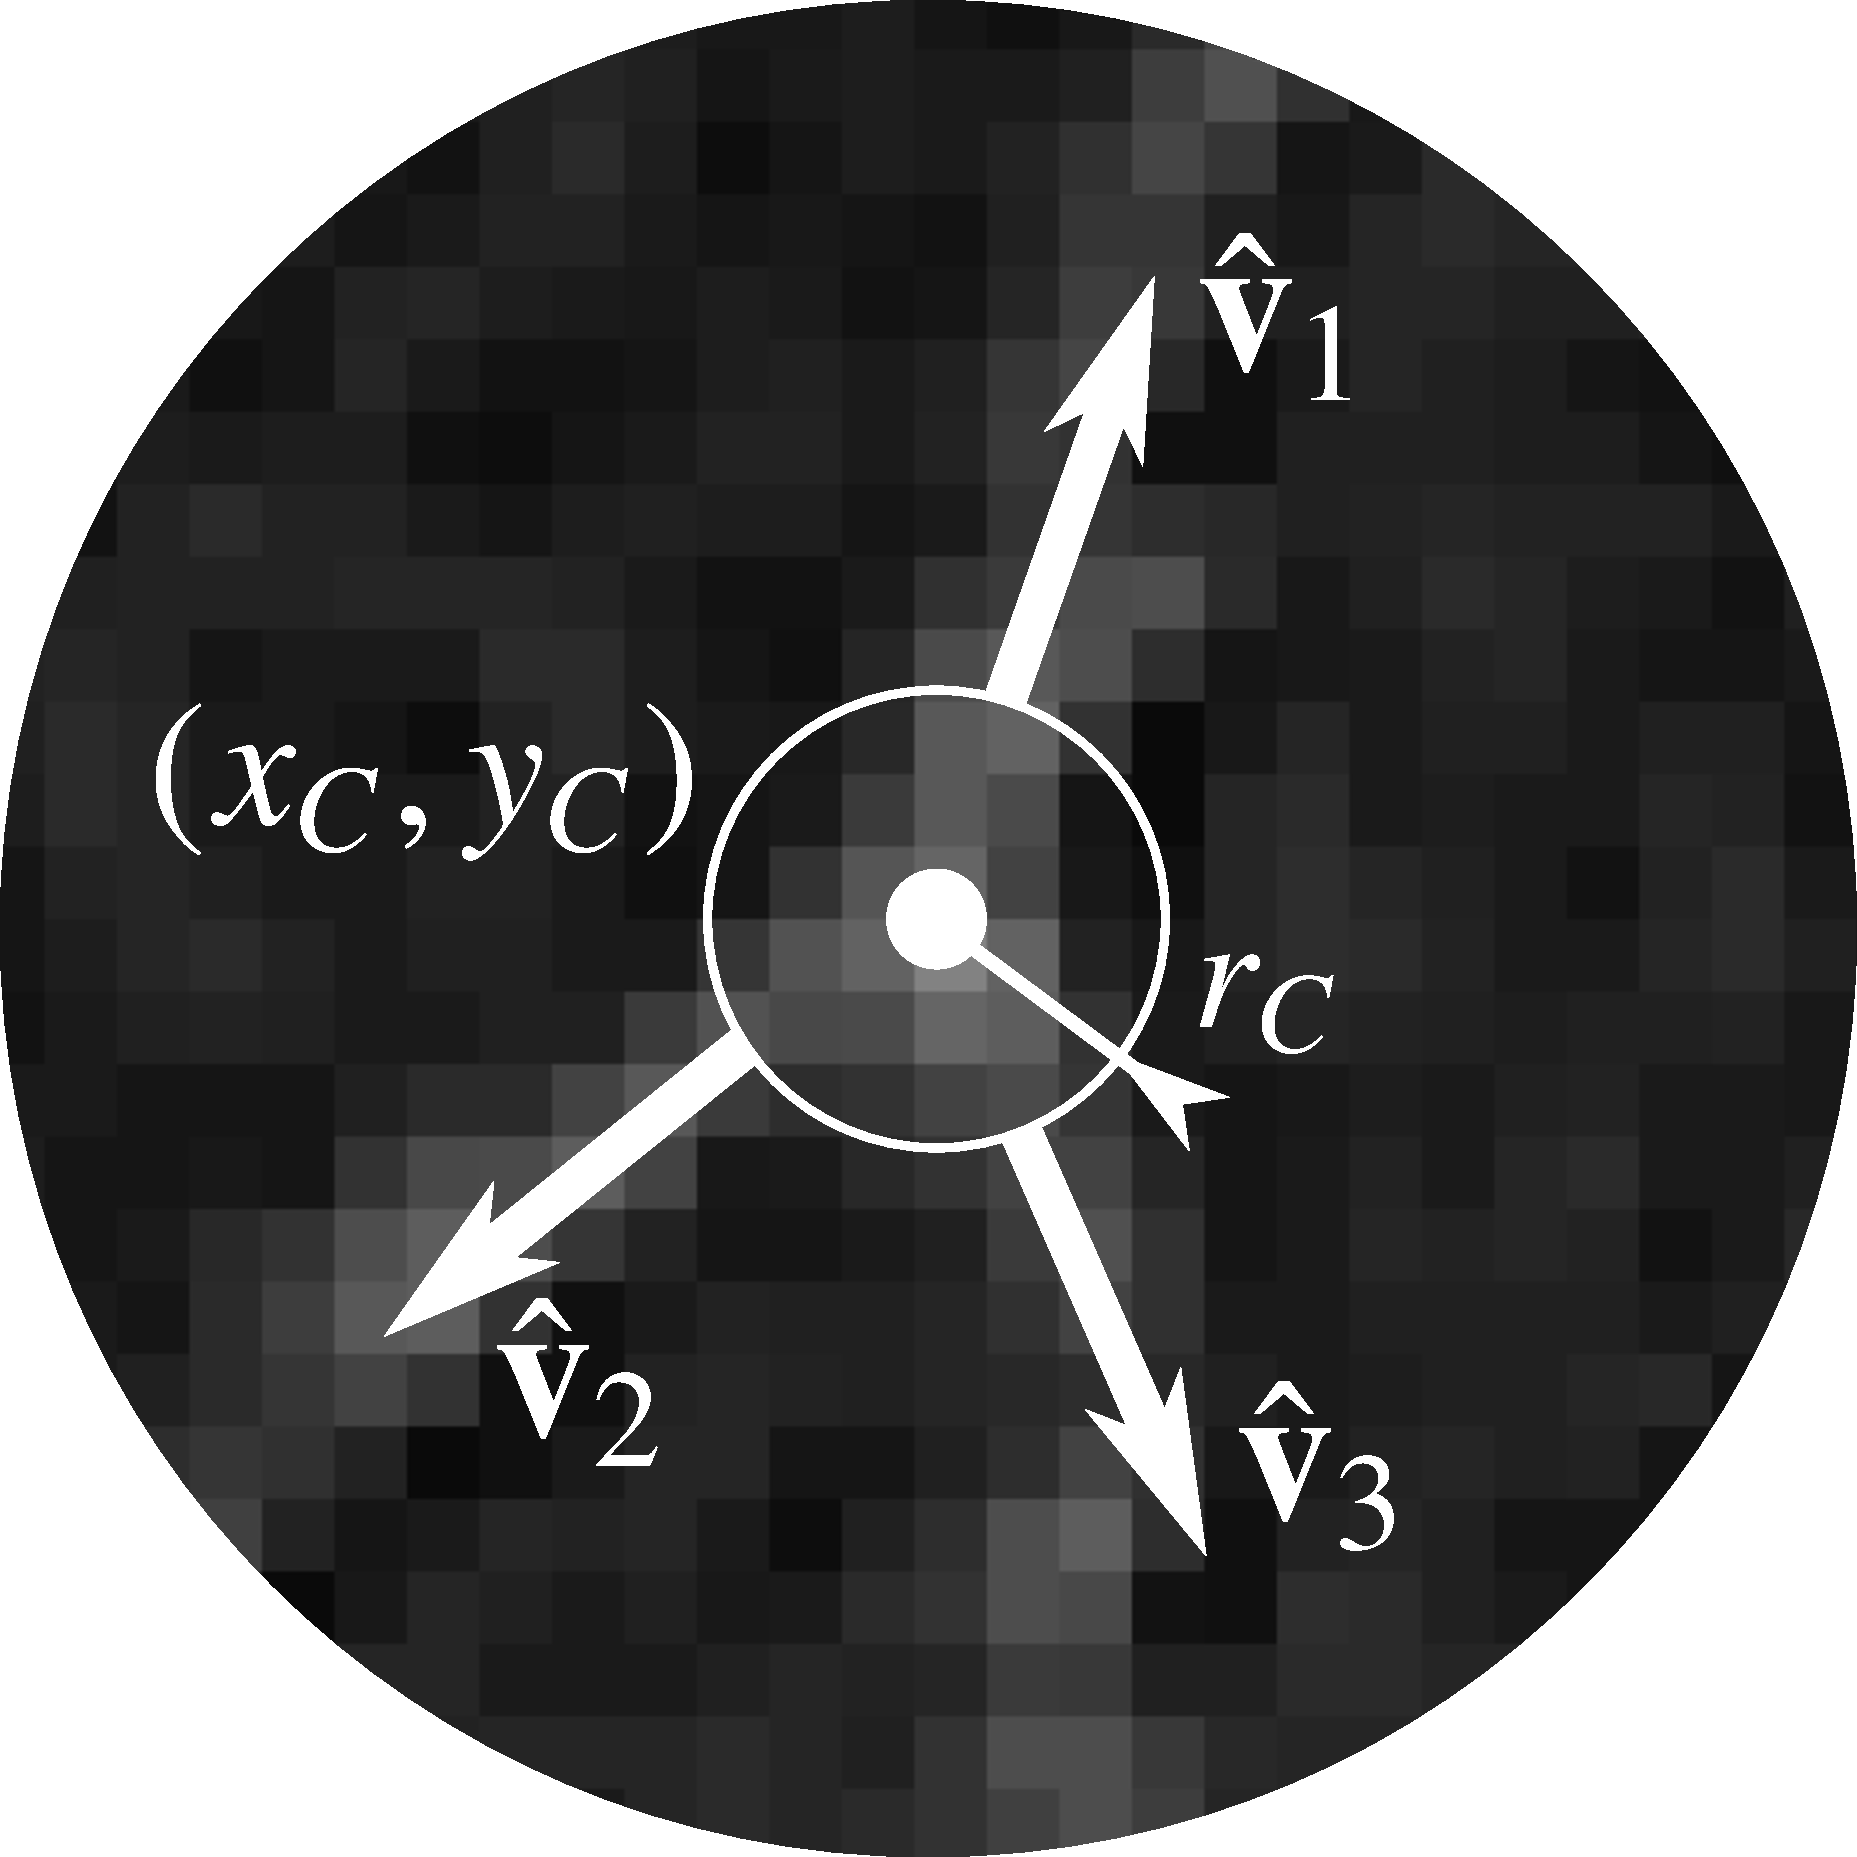
\includegraphics[height=9em]{cp-region} &
	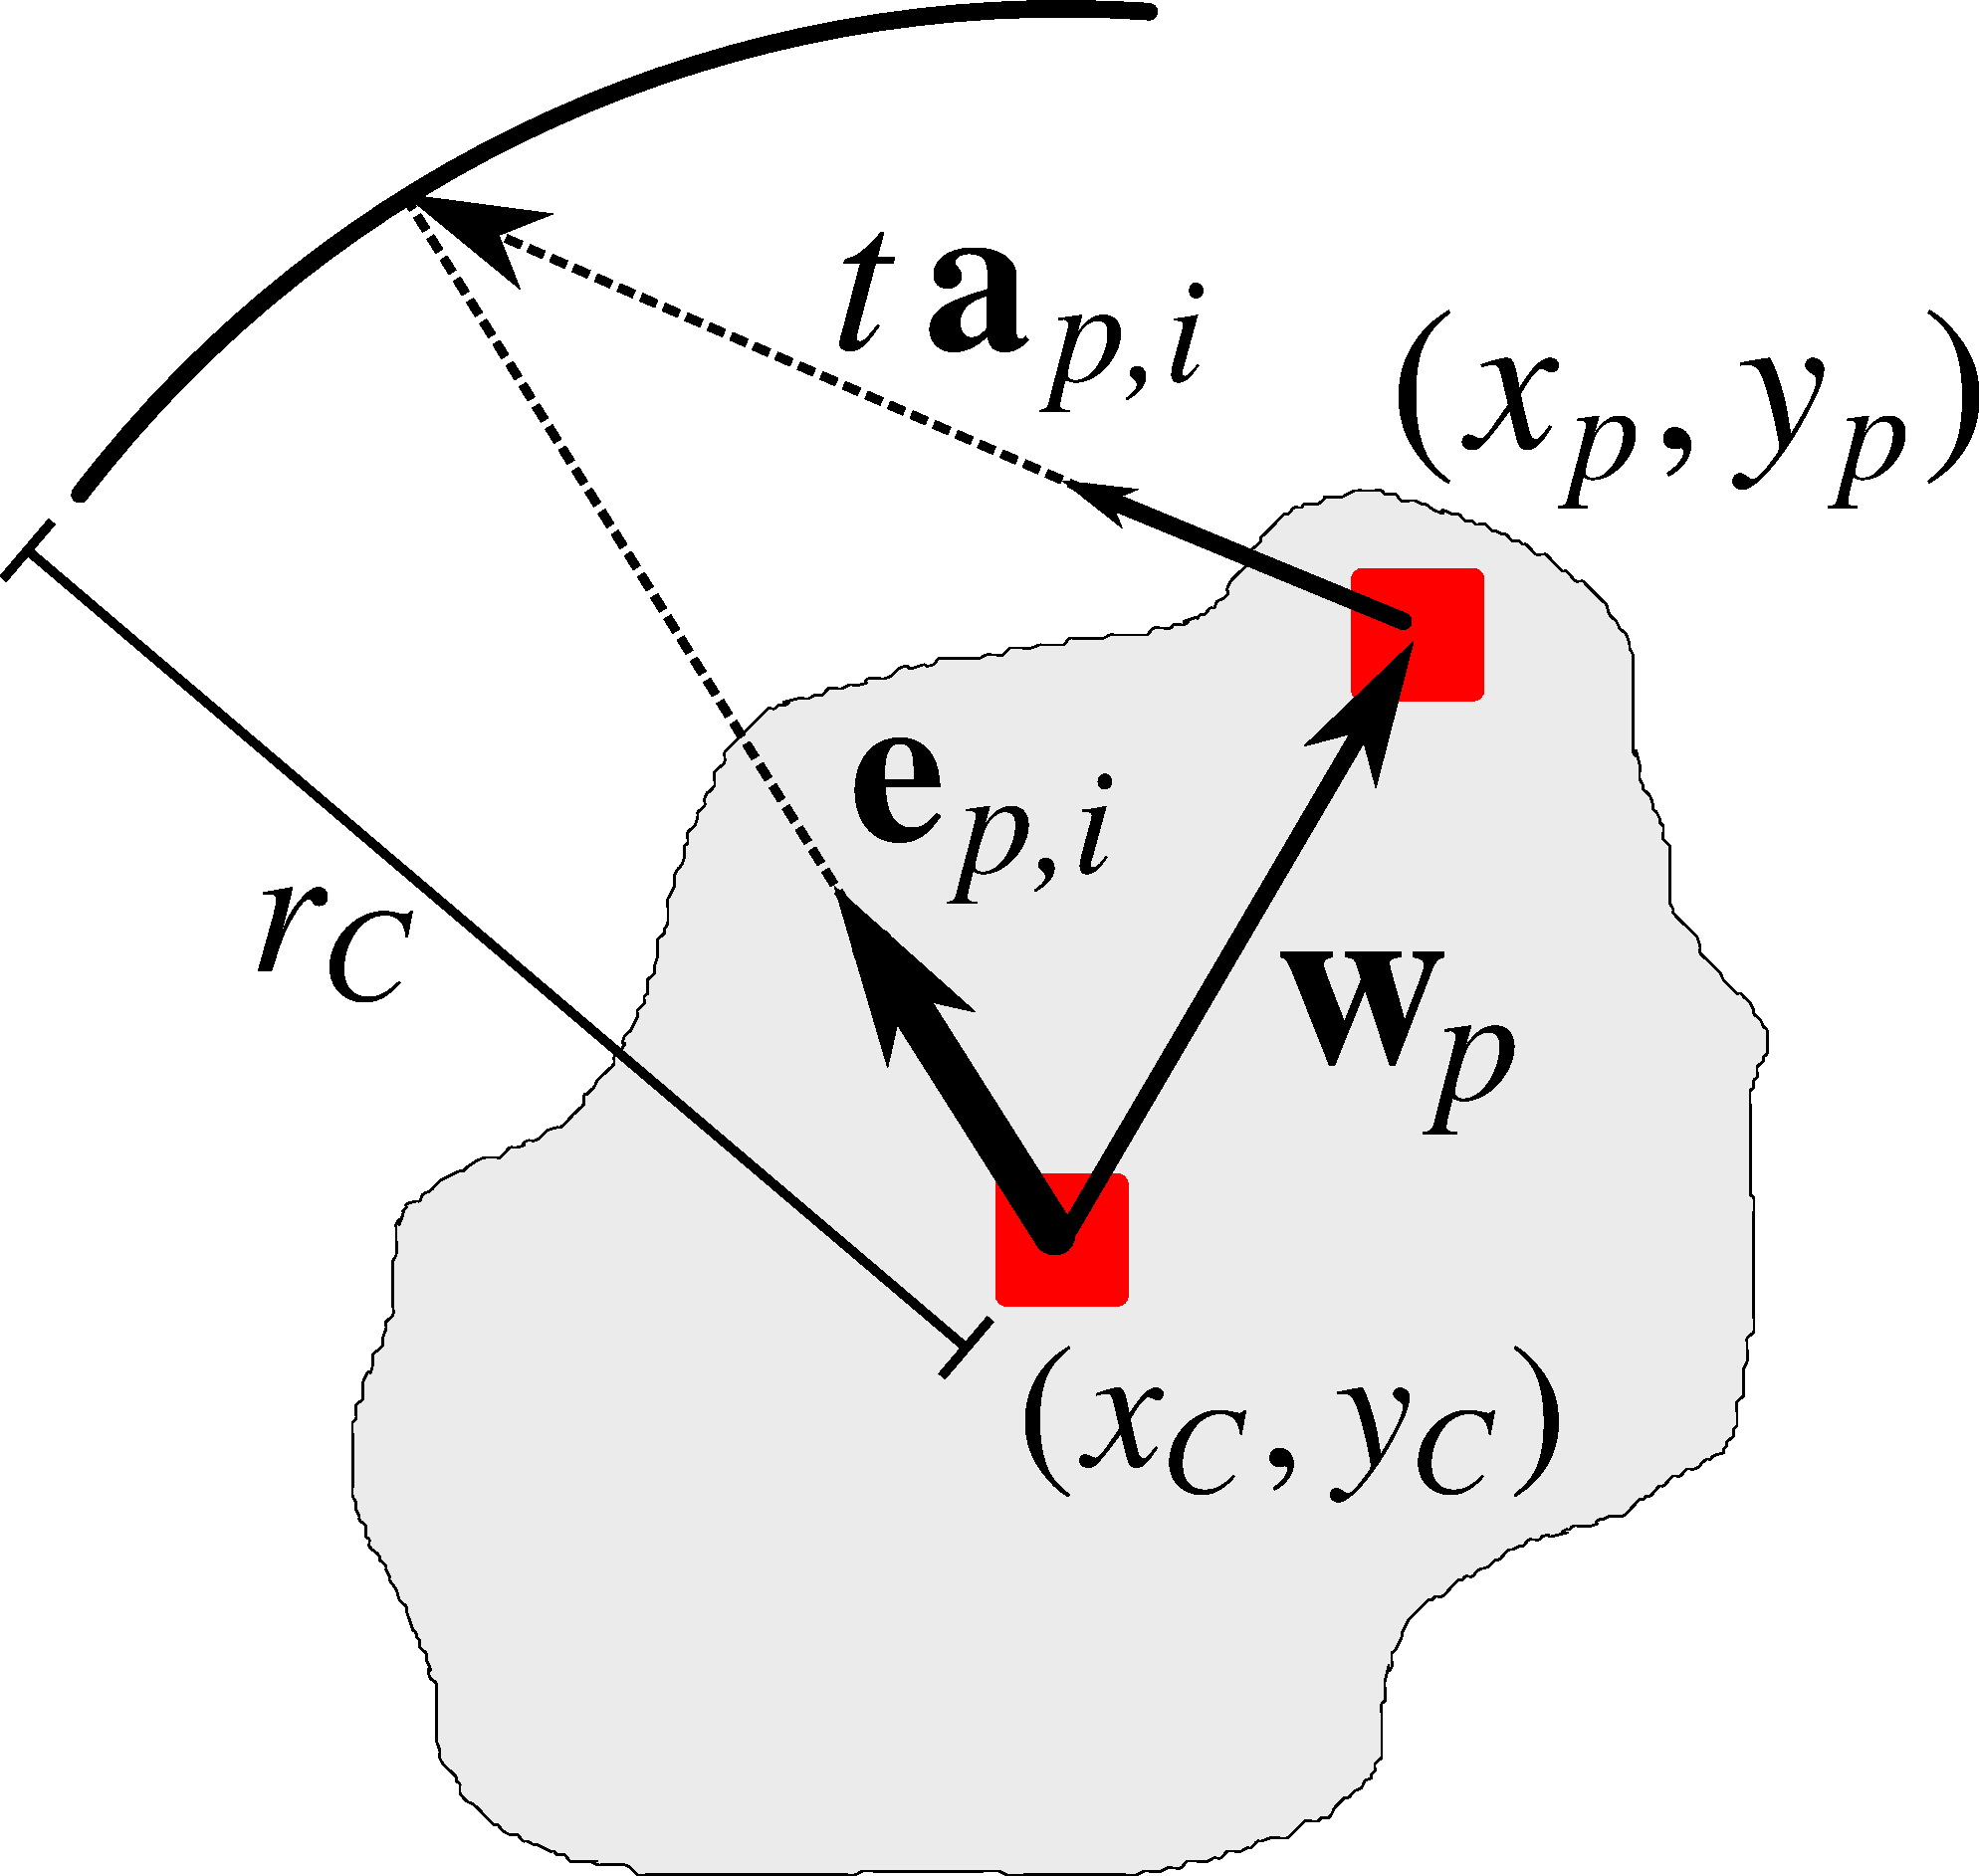
\includegraphics[height=9em]{cp-region-mapping}
	\end{tabular}
	\caption{Critical-point determination. A critical point is characterized by its type, centroid location $(x_C,y_C)$, radius $r_C$, and its main branch directions $\hat{\mathbf{v}}_i$ (left panel, in this case a bifurcation), aggregated from the pixels $(x_p,y_p)$ in the corresponding critical region (right panel).}
	\label{fig11}
\end{figure}
Due to noise, labeling imperfections, and structural ambiguities in the original image, the values of neighboring pixels in the maps may vary considerably, and direct thresholding usually does not give satisfactory results. To improve the robustness we first regularize the real-valued scores in the maps by means of local-average filtering with a radius of 3-5 pixels. Next, max-entropy based automatic thresholding \cite{kapur1985new} is applied to segment the maps, as in contrast with many other thresholding methods it was found to perform well in separating the large but relatively flat (low information) background regions from the much smaller but more fluctuating (high information) regions of interest. The resulting binary images are further processed using a standard connected components algorithm \cite{sonka2014image} to identify the critical-point regions.

Each critical region consists of a set of connected pixels $\mathbf{x}_p=(x_p,y_p)$, $p=1,\dots,N_p$, where $N_p$ denotes the number of pixels in the region. From these, the representative critical-point location $\mathbf{x}_C=(x_C,y_C)$ is calculated as:
\begin{equation}
\mathbf{x}_C=\frac{1}{N_p}\sum_{p=1}^{N_p}\mathbf{x}_p
\end{equation}
while the critical-point size is represented by the radius of the minimum circle surrounding the region:
\begin{equation}
r_C = \max_{p}\left\{||\mathbf{w}_p||\right\}
\end{equation}
where $\mathbf{w}_p=\mathbf{x}_p-\mathbf{x}_C$ (Fig.~\ref{fig11}). To obtain regularized estimates of the main branch directions $\hat{\mathbf{v}}_i$ for the critical point, the directions are aggregated corresponding to the angular profile peaks $\hat{\alpha}_i$ (Section~\ref{subsubsec:angular-profile}) of all the $\mathbf{x}_p$ in the region as follows. For each $\mathbf{x}_p$, $N_{\hat{\alpha}}\leq4$ angular profile peak direction vectors $\mathbf{a}_{p,i}=[\cos\hat{\alpha}_i(\mathbf{x}_p),\sin\hat{\alpha}_i(\mathbf{x}_p)]^T$ are found. Each of these vectors defines a line $\mathbf{a}(t)=\mathbf{x}_{p}+t\,\mathbf{a}_{p,i}$ parameterized by $t\in\mathbb{R}$. The projection of this line onto the circle $||\mathbf{x}-\mathbf{x}_C||^2=r^2_C$ is established by substituting $\mathbf{x}=\mathbf{a}(t)$ and solving for $t$. From this, the contributing unit vector is calculated (Fig.~\ref{fig11}):
\begin{equation}
\mathbf{e}_{p,i}=\frac{1}{r_C}(\mathbf{w}_{p}+t\,\mathbf{a}_{p,i})
\end{equation}
which points from $\mathbf{x}_C$ to the intersection point. This is done for all $p=1,\dots,N_p$ in the region and $i=1,\dots,N_{\hat{\alpha}}$ for each $p$, resulting in the set of vectors $\{\mathbf{e}_{p,i}\}$. Next, a recursive mean-shift clustering algorithm \cite{cheng1995mean} is applied to $\{\mathbf{e}_{p,i}\}$, which converges to a set $\{\hat{\mathbf{v}}_{i}\}$, where the cluster vectors $\hat{\mathbf{v}}_{i}$, $i=1,\dots,L$, represent the branches. For a critical region in $I_{\textrm{END}}$, only one main branch direction is needed, simply taken to be the direction $\hat{\mathbf{v}}_1$ to which the largest number of $\mathbf{e}_{p,i}$ were shifted. For a critical region in $I_{\textrm{JUN}}$, the $\hat{\mathbf{v}}_i$ (at least three) are taken as the main branch directions to which the largest number of $\mathbf{e}_{p,i}$ were shifted. These calculations are performed for all critical regions.

\section{Implementational Details}
\label{sec:implementation-details}
The method was implemented in the Java programming language as a plugin for the image processing and analysis tool ImageJ \cite{abramoff2004image, schneider2012nih}. Since the feature extraction step (Section~\ref{subsec:feature-extraction}), in particular the matched filtering for angular profile analysis, is quite computationally demanding, parallelization is applied in multiple ways to reduce the running time to acceptable levels (on the order of minutes on a regular PC). Specifically, the directional filtering was split between CPU cores, each taking care of a subset of the directions (depending on the number of available cores). After this, the angular profile analysis and calculation of the features was also split, with each core processing a subset of the foreground image locations. This was sufficient to run the experiments. Further improvement in running time (down to real-time if needed) could be achieved by mass parallelization using GPUs (graphical processing units) instead of CPUs.

Essential parameters that need to be set by the user are the scale parameters $k$ and $D$ (Section~\ref{subsubsec:angular-profile}) and the inflection points $L_{\mathrm{LOW}}$, $L_{\mathrm{HIGH}}$, $U_{\mathrm{LOW}}$, $U_{\mathrm{HIGH}}$, $C_{\mathrm{LOW}}$, and $C_{\mathrm{HIGH}}$ of the input membership functions used by fuzzy-logic module $\textrm{FL}_{1}$ (Section~\ref{sec:cp-detection}). In the showcased application, parameter $D$ is set to the expected neuron diameter in a given set of images while $k=0.7$ was kept fixed. The $L$ inflection points are always in the range $[0,1]$ since the corresponding feature (likelihood) is normalized. Based on ample experience with many data sets, $L_{\mathrm{LOW}}$ is typically set close to 0 and $L_{\mathrm{HIGH}}$ around $0.5$ (Fig.~\ref{fig7}). By contrast, the inflection points $U$ correspond to a feature (centerline bending energy) that is not normalized and may vary widely from $0$ to any positive value. To obtain sensible values for these, the histogram of all calculated energy values in the image is used. Parameter $U_{\mathrm{LOW}}$ is set to the threshold computed by the well-known triangle algorithm, while typically $U_{\mathrm{HIGH}}\gg U_{\mathrm{LOW}}$. It is useful to note that the membership functions defined by these parameters are inverted (Fig.~\ref{fig7}) such that the energy becomes a measure of smoothness. Finally, the $C$ inflection points correspond again to a feature (correlation) with a fixed output range $[-1,1]$. In practical applications they are usually set to $C_{\mathrm{LOW}}\in[0.1,0.5]$ and $C_{\mathrm{HIGH}}=0.95$  (Fig.~\ref{fig7}).

All other aspects of the method that could be considered as user parameters either follow directly from these essential parameters or are fixed to the standard values mentioned in the text. For example, the radius $r_d$ of the circular neighborhood in the foreground selection step (Section~\ref{subsubsec:foreground-selection}) can be set equal to $D$, and the standard deviation $\sigma_{\!D}$ of the Gaussian profile (Section~\ref{subsubsec:angular-profile}) can be set to $D/6$ to get a representative shape. Also, the output membership functions of $\textrm{FL}_1$ (input to $\textrm{FL}_2$) as well as the output membership functions of $\textrm{FL}_2$ are Gaussians with fixed levels and standard deviation (Section~\ref{sec:cp-detection}), as they are not essentially influencing the performance of the algorithm.
\begin{figure}%[t!]
	\centering
	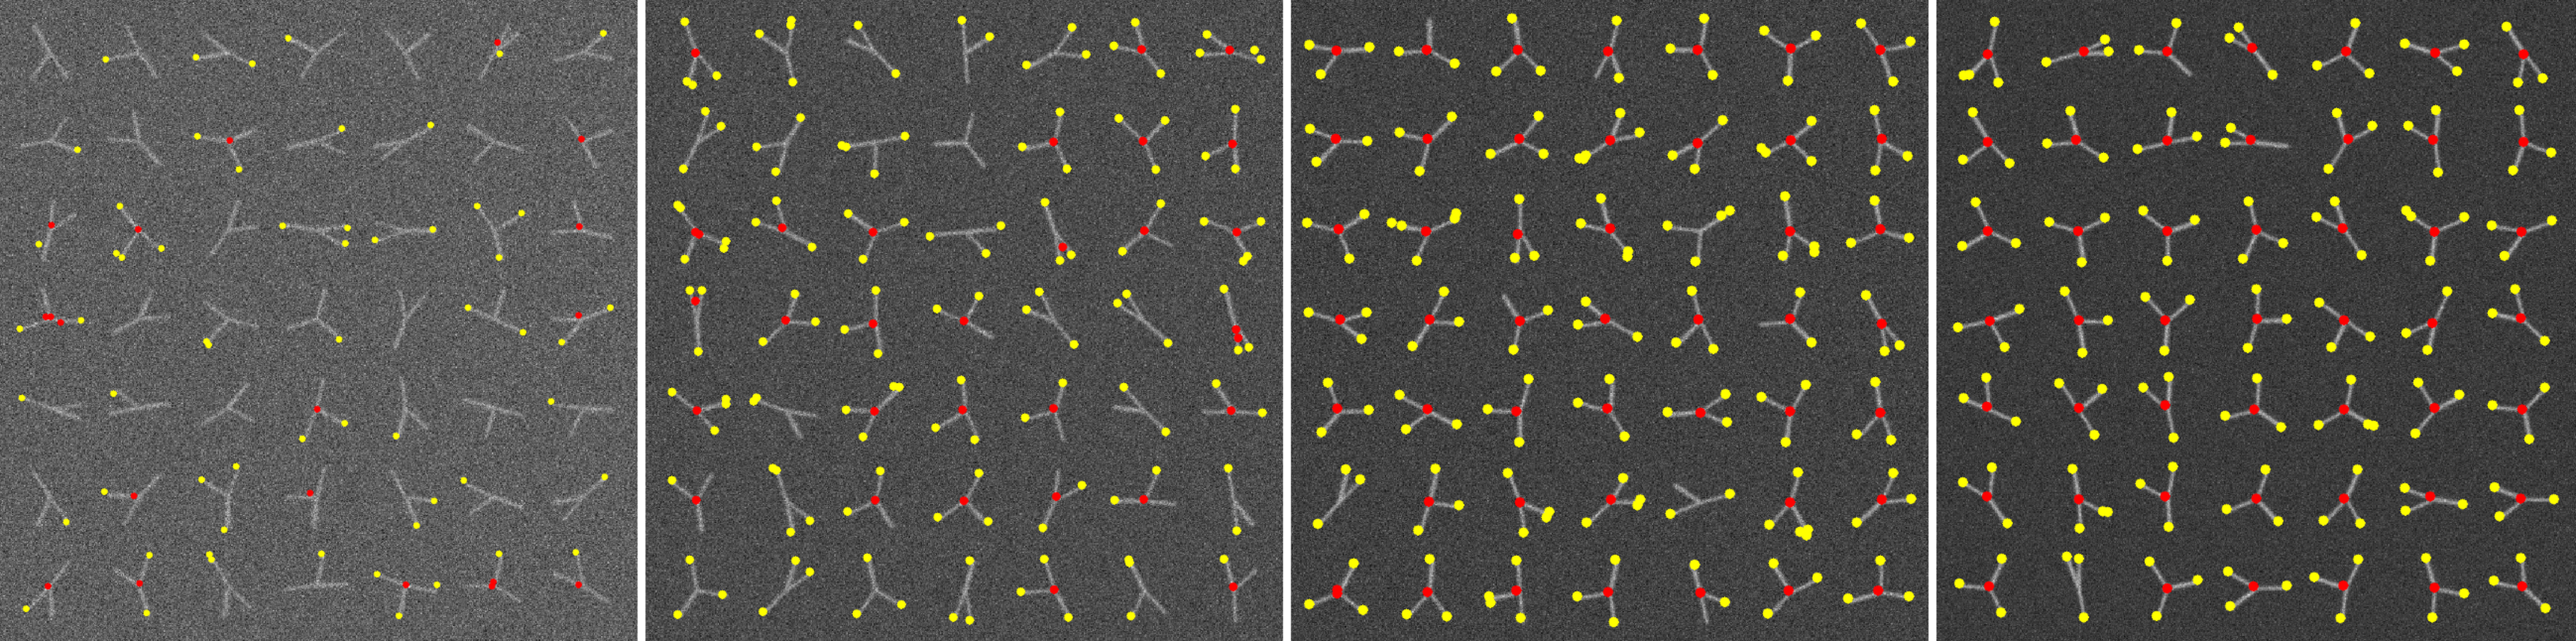
\includegraphics[width=\columnwidth]{fig12}
	\caption{Examples of simulated triplet images and detection results. Each triplet consists of three branches with different diameters which join at one end to form a bifurcation point and with the other ends being termination points. Images were generated at $\textrm{SNR}=2,3,4,5$ (left to right panel). The detection results with our method are indicated as red circles (bifurcation points) and yellow circles (termination points), where the radius of each circle reflects the size of the critical region found by our method.}
	\label{fig12}
\end{figure}
\section{Experimental Results}
\label{sec:experiments}
To evaluate the performance of Neuron Pinpointer method in correctly detecting and classifying neuronal critical points, experiments with simulated images (using the ground truth available from the simulation) as well as with real fluorescence microscopy images (using manual annotation as the gold standard) have been performed. After outlining the performance measures (Section \ref{subsec:performance-measures}), the results of the evaluation on simulated images are presented, including the synthetic triplets (Section \ref{subsec:experiments-triplets}) and synthetic neurons (Section \ref{subsec:experiments-simulated}), and on real neuron images (Section \ref{subsec:experiments-real}). Finally, the results of a comparison of the method with two other methods (Section \ref{subsec:comparison}) is showcased.
\subsection{Performance Measures}
\label{subsec:performance-measures}
Performance was quantified by counting the correct and incorrect hits and the misses of the detection with respect to the reference data. More specifically, the true-positive (TP), false-positive (FP), and the false-negative (FN) critical-point detections had been counted, and used to calculate the recall $\textrm{R}=\textrm{TP}/(\textrm{TP}+\textrm{FN})$ and precision $\textrm{P}=\textrm{TP}/(\textrm{TP}+\textrm{FP})$. Both R and P take on values in the range from $0$ (meaning total failure) to $1$ (meaning flawless detection). They are commonly combined in the F-measure \cite{powers2011evaluation}, defined as the harmonic mean of the two: $\textrm{F}=2\,\textrm{R}\,\textrm{P}/(\textrm{R}+\textrm{P})$. The F-measure was computed separately for each type of critical points considered in this paper, yielding $\textrm{F}_{\textrm{END}}$ for terminations and $\textrm{F}_{\textrm{JUN}}$ for junctions. As a measure of overall performance, the harmonic mean of the two F-measures: $\textrm{F}_{\textrm{BOTH}}=2\,\textrm{F}_{\textrm{END}}\,\textrm{F}_{\textrm{JUN}}/(\textrm{F}_{\textrm{END}}+\textrm{F}_{\textrm{JUN}})$ is also computed.
\begin{figure}
	\centering
	\begin{tabular}{c@{\hspace{1em}}c@{\hspace{1em}}}
	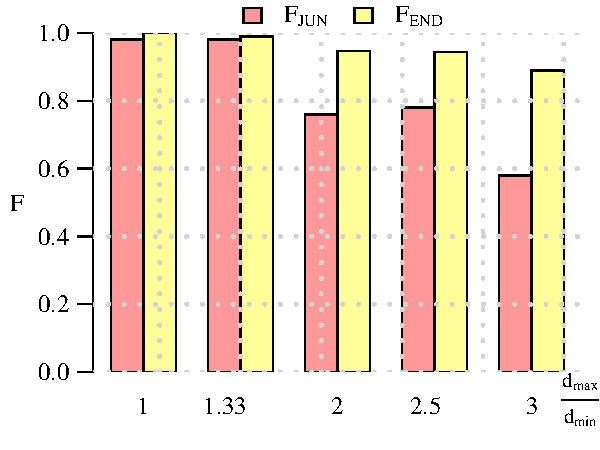
\includegraphics[width=0.4\columnwidth]{triplets_fjun_fend_vs_pratio} &
	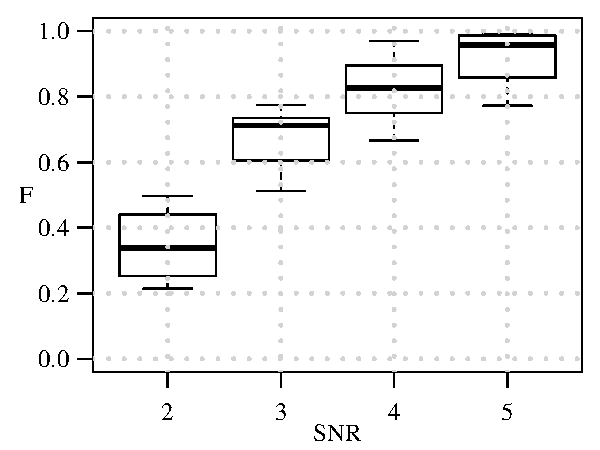
\includegraphics[width=0.4\columnwidth]{triplets_fboth_vs_snr}
	\end{tabular}
	\caption{Performance of the method in detecting terminations and junctions in simulated images of triplets. The values of $\textrm{F}_{\textrm{END}}$ and $\textrm{F}_{\textrm{JUN}}$ are shown (left panel) for the various branch diameter ratios $d_{\max}/d_{\min}$ at $\textrm{SNR} = 4$. The distribution of $\textrm{F}_{\textrm{BOTH}}$ values is shown as a box plot (right panel) for the various SNR levels.}
	\label{fig13}
\end{figure}

\subsection{Evaluation on Simulated Triplet Images}
\label{subsec:experiments-triplets}
Before considering full neuron imagery the performance of the method was first evaluated at detecting terminations and junctions in a very basic configuration as a function of image quality. To this end, a triplet model was used, consisting of a single junction modeling a bifurcation, having three branches with arbitrary orientations (angular intervals) and diameters (Fig.~\ref{fig12}). Orientations were randomly sampled from a uniform distribution in the range $[0, 2\pi]$ while prohibiting branch overlap. Since in principle the directional filtering step (Section \ref{subsubsec:angular-profile}) uses a fixed kernel size $D$, the intent was to investigate the detection robustness for varying ratios $d_{\max}/d_{\min}$ between the maximum and the minimum branch diameter in a triplet. For such experiment, $1,0.33,2,2.5,3$ ratios were considered by taking normalized diameter configurations ($d_1,d_2,d_3$) = (0.33,0.33,0.33), (0.3,0.3, 0.4), (0.2, 0.4,0.4), (0.2,0.3,0.5), (0.2,0.2,0.6), where in each case the actual smallest diameter was set to 3 pixels (the resolution limit) and the other diameters were scaled accordingly. A set of images was simulated for each configuration containing $1,000$ well-separated triplets for signal-to-noise ratio levels $\textrm{SNR}=2$, $3$, $4$, $5$ (see cropped examples in Fig.~\ref{fig12}). These levels are chosen knowing that $\textrm{SNR}=4$ is a critical level in other detection problems \cite{smal2010quantitative, chenouard2014objective}. Poisson noise was used in simulating fluorescence microscopy imaging of the triplets. The obtained results of this experiment (Fig.~\ref{fig13}) lead to the conclusion that the method is fairly robust for diameter ratios $d_{\max}/d_{\min}\leq2\frac{1}{2}$ and an image quality of $\textrm{SNR} \geq 4$. Based on the detection rates, it is also possible to draw a conclusuion that our method is somewhat better in detecting terminations than detecting junctions in synthetic images. Example detection results for $d_{\max}/d_{\min}\leq2$ for the considered SNR levels are shown in Fig.~\ref{fig12}.

\begin{figure}
	\centering
	\begin{tabular}{c@{\hspace{0.1em}}c@{\hspace{0.1em}}c@{\hspace{0.1em}}c@{\hspace{0.1em}}}
		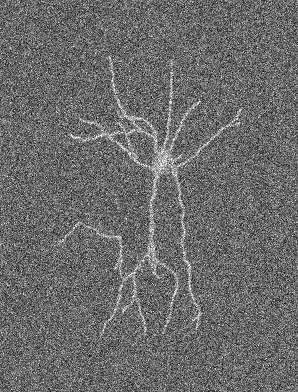
\includegraphics[width=0.2\columnwidth]{dekoninck-snr-2} &
		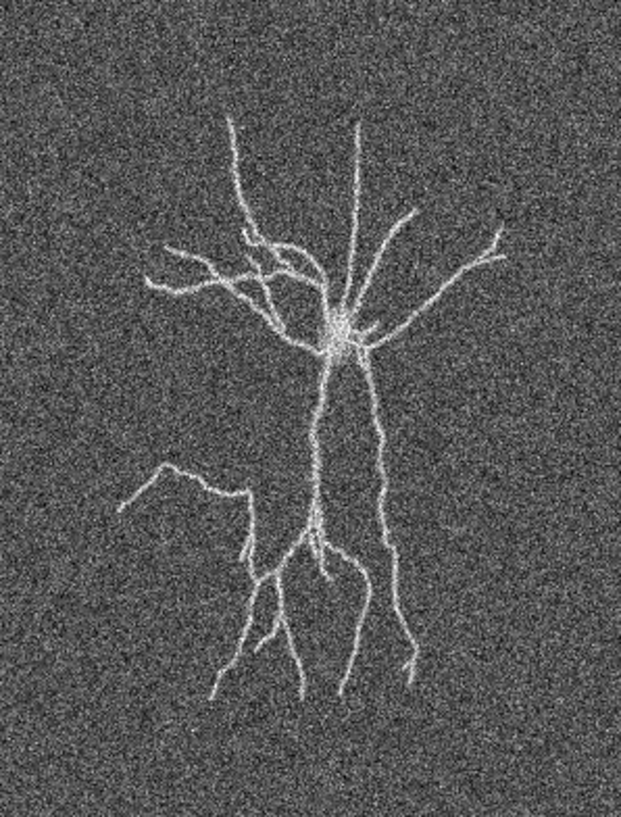
\includegraphics[width=0.2\columnwidth]{dekoninck-snr-3} &
		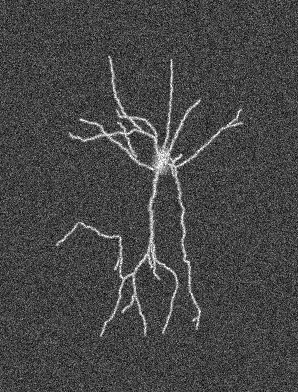
\includegraphics[width=0.2\columnwidth]{dekoninck-snr-4} &
		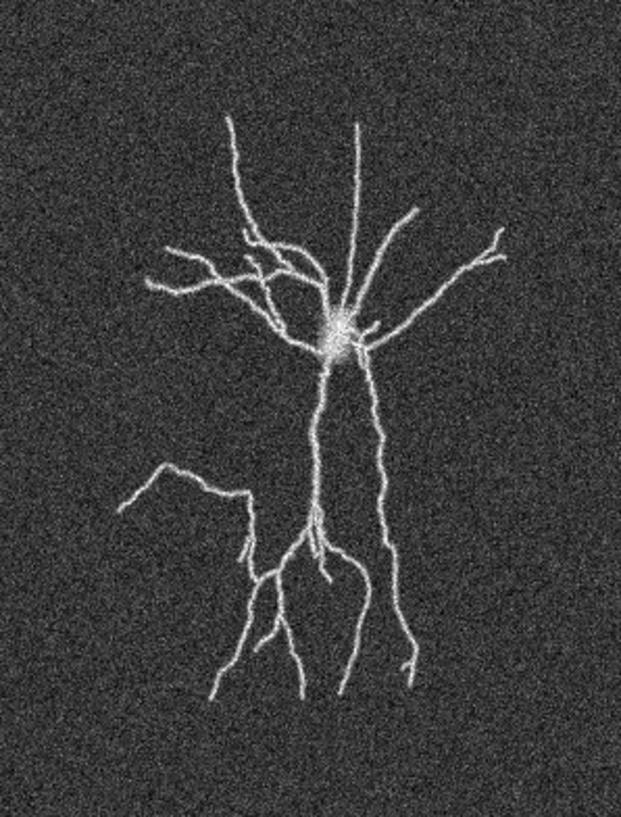
\includegraphics[width=0.2\columnwidth]{dekoninck-snr-5}\\%[0.1ex]
		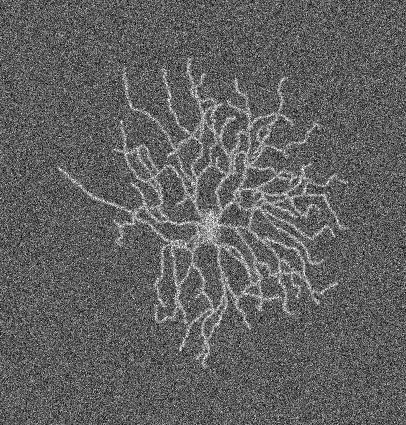
\includegraphics[width=0.2\columnwidth]{strettoi-snr-2} &
		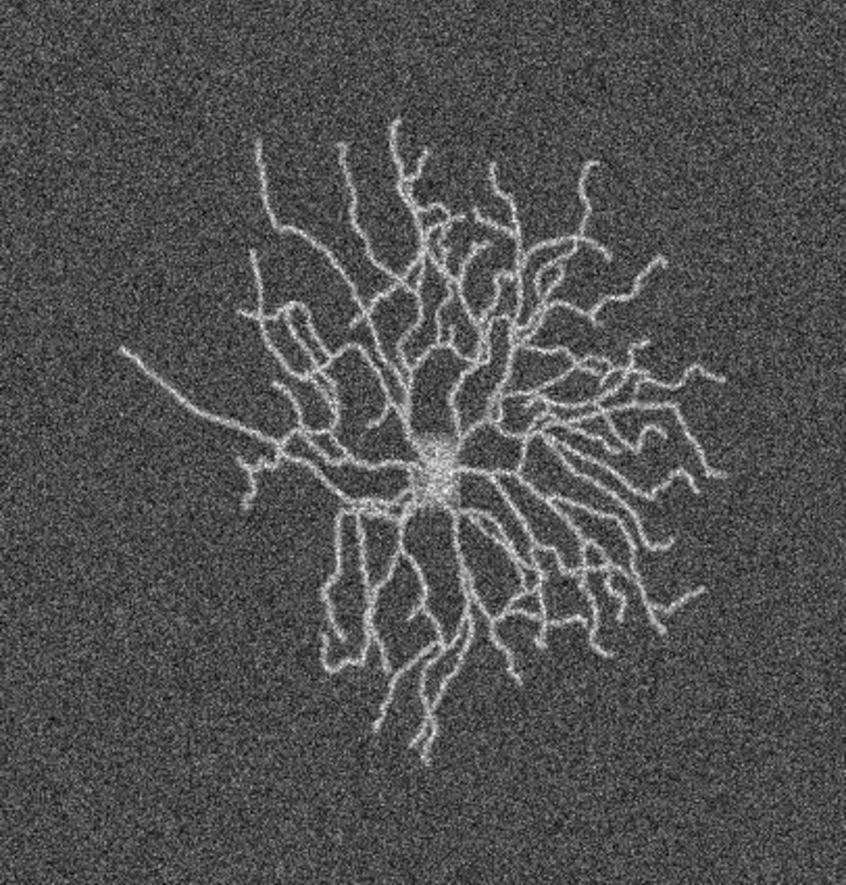
\includegraphics[width=0.2\columnwidth]{strettoi-snr-3} &
		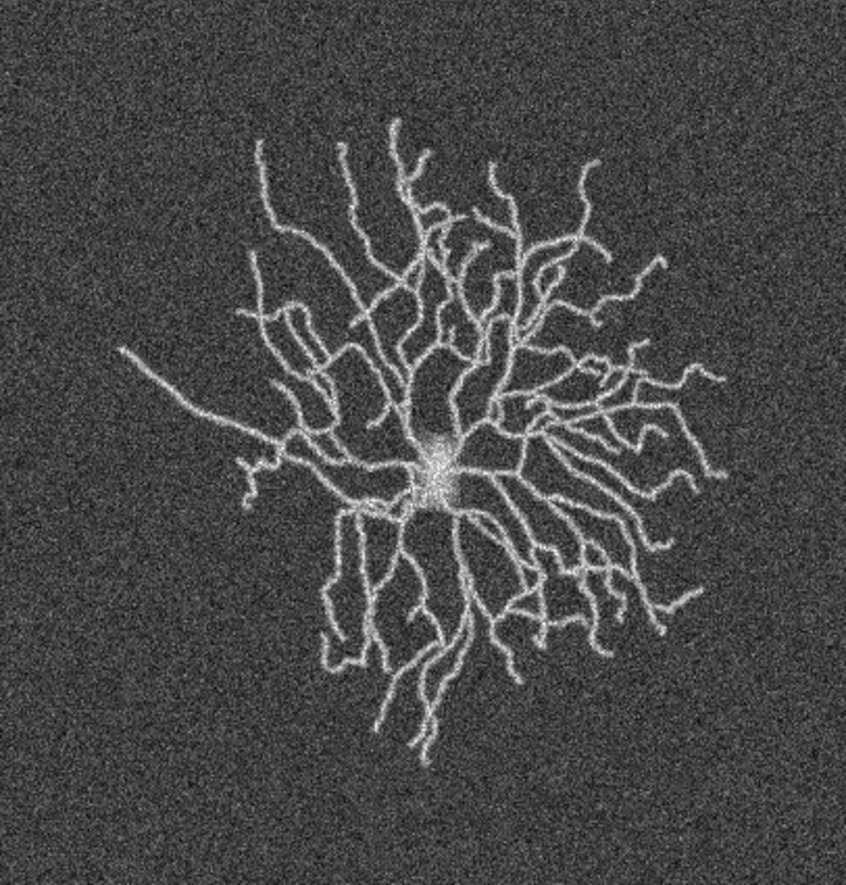
\includegraphics[width=0.2\columnwidth]{strettoi-snr-4} &
		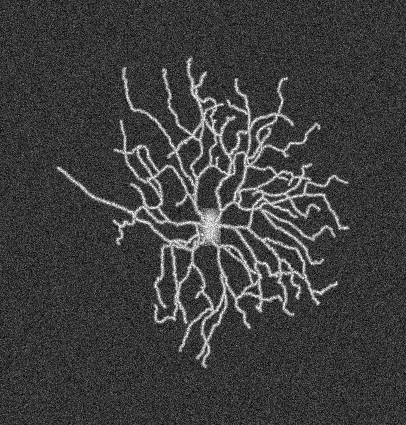
\includegraphics[width=0.2\columnwidth]{strettoi-snr-5}\\%[0.1ex]
		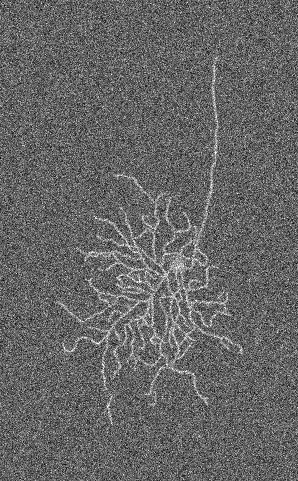
\includegraphics[width=0.2\columnwidth]{masland-snr-2} &
		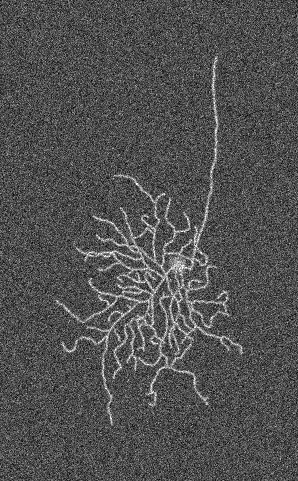
\includegraphics[width=0.2\columnwidth]{masland-snr-3} &
		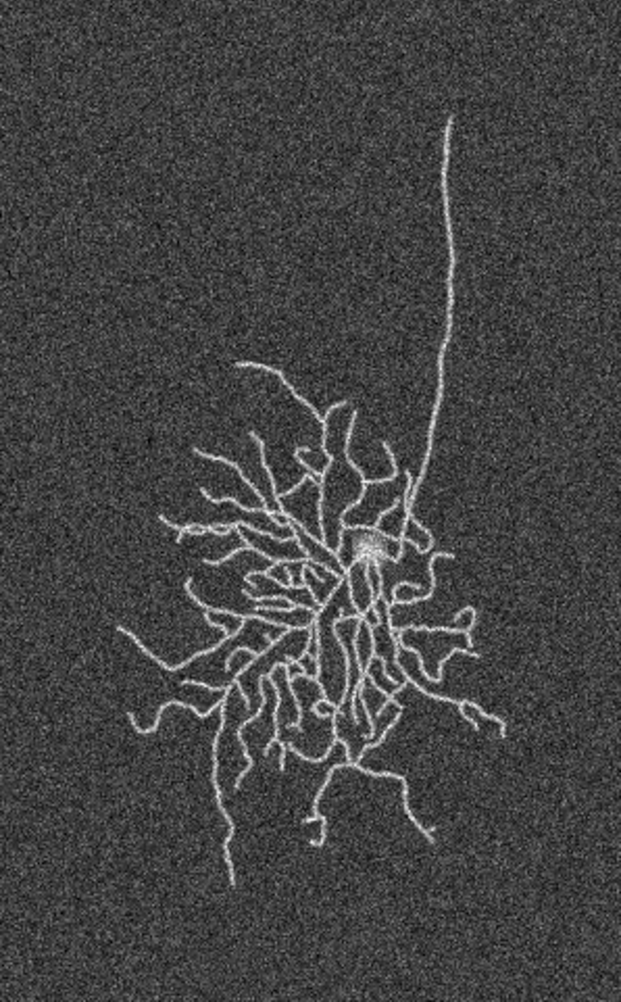
\includegraphics[width=0.2\columnwidth]{masland-snr-4} &
		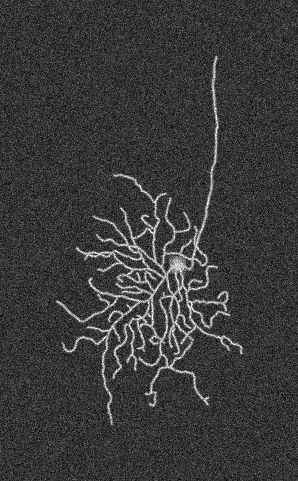
\includegraphics[width=0.2\columnwidth]{masland-snr-5}\\%[0.1ex]
		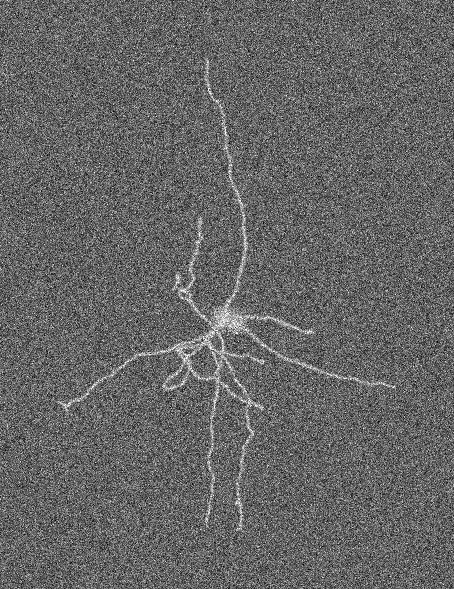
\includegraphics[width=0.2\columnwidth]{burdakov-snr-2} &
		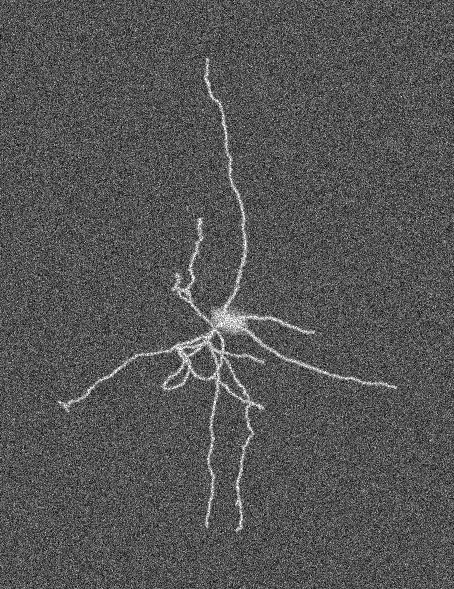
\includegraphics[width=0.2\columnwidth]{burdakov-snr-3} &
		\includegraphics[width=0.2\columnwidth]{burdakov-snr-4} &
		\includegraphics[width=0.2\columnwidth]{burdakov-snr-5}\\%[0.1ex]
		\includegraphics[width=0.2\columnwidth]{jacobs-snr-2} &
		\includegraphics[width=0.2\columnwidth]{jacobs-snr-3} &
		\includegraphics[width=0.2\columnwidth]{jacobs-snr-4} &
		\includegraphics[width=0.2\columnwidth]{jacobs-snr-5}
	\end{tabular}
	\caption{Examples of simulated neuron images based on expert reconstructions from the NeuroMorpho.Org database. The images show a wide range of morphologies (one type per row) and image qualities of $\textrm{SNR}=2$, $3$, $4$, $5$ (from left to right per row).}
	\label{fig14}
\end{figure}

\begin{figure}
	\centering
	\begin{tabular}{c@{\hspace{1em}}c@{\hspace{1em}}}
		\includegraphics[width=0.4\columnwidth]{nmorpho_snr4} &
		\includegraphics[width=0.4\columnwidth]{nmorpho_snr}
	\end{tabular}
	\caption{Performance of the method in detecting terminations and junctions in 30 simulated images of neurons. The distributions of the $\textrm{F}_\textrm{END}$, $\textrm{F}_\textrm{JUN}$, and $\textrm{F}_\textrm{BOTH}$ values are shown as box plots for $\textrm{SNR}=4$ (left panel) and in addition the distribution of $\textrm{F}_\textrm{BOTH}$ is shown for $\textrm{SNR}=2$, $3$, $4$, $5$ (right panel).}
	\label{fig15}
\end{figure}

\subsection{Evaluation on Simulated Neuron Images}
\label{subsec:experiments-simulated}
To evaluate the method on more complex images, with the known ground truth, the imaging of complete neurons was simulated. Although there are various ways this could be done \cite{koene2009netmorph, vasilkoski2009detection}, the existing expert reconstructions from the NeuroMorpho.Org database \cite{ascoli2007neuromorpho} were used. A total of 30 reconstructions from different neuron types were downloaded as SWC files \cite{cannon1998line}, in which the reconstructions are represented as a sequence of connected center-point locations in 3D with corresponding radii in micrometers. Fluorescence microscopy images were generated from these reconstructions in 2D by using a Gaussian point-spread function model and Poisson noise to emulate diffraction-limited optics and photon statistics. For each reconstruction, the images of $\textrm{SNR}=2$, $3$, $4$, $5$ (Fig.~\ref{fig14}) were generated. The simulated images of neurons are obtained this way, each with the exactly known location of the termination and junction point, extrapolated from the source SWC file.
\begin{figure}
	\centering
		\includegraphics[width=0.9\textwidth,height=0.9\textheight,keepaspectratio]{det_nmorpho}
			\caption{Example detections for simulated neuron images at $\textrm{SNR}=4$. The showcased images are contrast enhanced and show the detected terminations (yellow circles) and junctions (red circles) as overlays with fixed radius for better visibility. The value of $\textrm{F}_\textrm{BOTH}$ in these examples is (a) 0.69, (b) 0.85, (c) 0.85, (d) 0.77, (e) 0.75, (f) 0.68, (g) 0.86.}
	\label{fig16}
\end{figure}
The evaluation results (Fig.~\ref{fig15}) confirm the conclusion from the experiments on triplets that the method performs well for $\textrm{SNR} \geq 4$ and is somewhat better in detecting terminations than detecting junctions. For $\textrm{SNR} = 4$ the performance for junction detection is $\textrm{F}_{\textrm{JUN}} \approx 0.85$ while for termination detection $\textrm{F}_{\textrm{END}} \approx 0.95$. The higher performance for termination detection may be explained by the fact that the underlying image structure is usually less ambiguous (a single line-like structure surrounded by darker background) than in the case of junctions (multiple line-like structures that are possibly very close to each other). Example detection results are shown in Fig.~\ref{fig16}.
\begin{figure}
	\centering
	\includegraphics[width=0.4\columnwidth]{overview_real}
	\caption{Performance of the method in detecting terminations and junctions in 30 real fluorescence microscopy images of neurons. The distributions of the $\textrm{F}_\textrm{END}$, $\textrm{F}_\textrm{JUN}$, and $\textrm{F}_\textrm{BOTH}$ values for all images together are shown as box plots.}
	\label{fig17}
\end{figure}
\subsection{Evaluation on Real Neuron Images}
\label{subsec:experiments-real}
As the ultimate test case, the method was also evaluated on real fluorescence microscopy images of neurons from a published study \cite{steiner2002overexpression}. A total of 30 representative images were taken and expert manual annotations of the critical points were obtained to serve as the gold standard in this experiment. Naturally, real images are generally more challenging than simulated images, as they contain more ambiguities due to labeling and imaging imperfections, and thus the lower performance was expected. Since in this case there is no control over the SNR in the images, the detection results are reported for all images together. The evaluation results (Fig.~\ref{fig17}) indicate that the median performance in detecting critical points is $\textrm{F}_{\textrm{JUN}}=0.81$ for junctions and $\textrm{F}_{\textrm{END}}=0.73$ for terminations while $\textrm{F}_{\textrm{BOTH}}=0.76$. As expected, these numbers are lower than those of the simulated neuron images. Surprisingly, the junction detection performance with the real images is better than the termination detection which had not been the case with the synthetic neurons. A possible explanation for this could be that in the simulated images a constant intensity was used for the neuron branches, as a result of which terminations are as bright as junctions but much less ambiguous due to a clear background, while in the real images the terminations are usually much less clear due to labeling imperfections and the fact that the branch tips tend to be thinner and thus less bright than the junctions. This illustrates the limitations of the simulations. Example detection results are shown in the Fig.~\ref{fig18}.
\begin{figure}
	\centering
	\includegraphics[width=0.7\textwidth,height=0.7\textheight,keepaspectratio]{det_real}
	\caption{Example detections for four real neuron images. The detected terminations (yellow circles) and junctions (red circles) are shown as overlays with fixed radius for better visibility. The value of $\textrm{F}_\textrm{BOTH}$ in these examples is (a) 0.82, (b) 0.78, (c) 0.68, (d) 0.65.}
	\label{fig18}
\end{figure}
\subsection{Comparison With Other Methods}
\label{subsec:comparison}
Finally the performance comparison of the Neuron Pinpointer method against other methods is conduct. In lack of availability of other methods explicitly designed to detect and classify critical points in neuron images before reconstruction, two existing software tools relevant in this context were considered and their implicit detection capabilities compared with the presented explicit method. If NP indicates better performance, this would indicate that the existing methods may be improved by exploiting the output of the method.
\begin{figure}
	\centering
	\begin{tabular}{c@{\hspace{1em}}c@{\hspace{1em}}c@{\hspace{1em}}}
	\includegraphics[width=0.3\columnwidth]{compareJUN_all}
	\includegraphics[width=0.3\columnwidth]{compareEND_all}
	\includegraphics[width=0.3\columnwidth]{compareBOTH_all}
	\end{tabular}
	\caption{Critical-point detection performance of our method (NP) compared to two other methods (AS and APP2). The median values of $\textrm{F}_{\textrm{JUN}}$ (left plot) are 0.81 (NP), 0.65 (AS), and 0.47 (APP2). The median values of $\textrm{F}_{\textrm{END}}$ (middle plot) are 0.73 (NP), 0.28 (AS), and 0.21 (APP2). Finally, the median values of $\textrm{F}_{\textrm{BOTH}}$ (right plot) are 0.76 (NP), 0.35 (AS), and 0.29 (APP2).}
	\label{fig19}
\end{figure}
The first tool, AnalyzeSkeleton (AS)\footnote{available from http://fiji.sc/AnalyzeSkeleton} \cite{arganda20103d}, is an ImageJ plugin for finding and counting all end-points and junctions in a skeleton image. To obtain skeleton images of the neuron images used for this study, the related skeletonization method\footnote{http://fiji.sc/Skeletonize3D} inspired by an advanced thinning algorithm \cite{lee1994building} was used. The input for the latter is a binary image obtained by segmentation based on smoothing (to reduce noise) and thresholding. We considered a range of smoothing scales in the experiments and manually selected thresholds as well as automatically determined thresholds using the following algorithms from ImageJ: Intermodes, Li, MaxEntropy, RenyiEntropy, Moments, Otsu, Triangle, and Yen. All of these were tried in combination with the AS method and the highest F-scores were used.

The second tool, All-Path-Prunning (APP2) \cite{xiao2013app2}, is a plugin for Vaa3D\footnote{available from http://www.vaa3d.org/} \cite{peng2010v3d, peng2014extensible}. It was not designed specifically for a priori critical-point detection but for fully automatic neuron reconstruction. Nevertheless, in producing a tree representation of a neuron, the reconstruction algorithm must somehow identify the branch end-points and junctions, and for aforementioned experiments it is straightforward to retrieve them from the SWC output files. In principle, any neuron reconstruction method is also implicitly a critical-point detection method, and its performance could be quantified by comparing the output tree nodes with the reference data. The interesting question is whether an explicit detector such as NP outperforms the implicit detection carried out in a tool such as APP2. The user parameters of the tool were manually adjusted to get optimal performance in our experiments.

A comparison of the F-scores of NP, AS, and APP2 for the 30 real neuron images used throughout the experiments is presented in Fig.~\ref{fig19}. The plots indicate that the detection rates of the NP method are substantially higher than those of AS and APP2. The difference is especially noticeable for the termination points. More specifically, the difference between $\textrm{F}_{\textrm{END}}$ and $\textrm{F}_{\textrm{JUN}}$ is relatively small for NP, but much larger for both AS and APP2. This indicates a clear advantage of using presented explicit and integrated approach for detecting critical points, as accurate neuron reconstruction requires accurate detection of both junctions and terminations. However, with the current implementation, this advantage does come at a cost: timing of the three methods on a standard PC (with Intel Core i7-2630QM 2GHz CPU and 6 GB total RAM) revealed that with our images of $10^5$ to $10^6$ pixels in size, NP took about 40 seconds per image on average, while both AS and APP2 took only about 1.5 seconds per image. Fortunately, since virtually all the computation time of our method is spent in the directional filtering step, which is highly parallelizable, this cost can be reduced to any desired level by employing many-core hardware (such as GPUs).
\section{Conclusions} 
\label{sec:conclusions}
A novel method for solving the important problem of detecting and characterizing critical points in the tree-like structures in neuron microscopy images is presented. Based on directional filtering and feature extraction in combination with a two-stage fuzzy-logic based reasoning system, it provides an integrated framework for the simultaneous identification of both terminations and junctions. From the experimentation on simulated as well as real fluorescence microscopy images, it is possible to conclude that the method achieves substantially higher detection rates than the ones that can be inferred from existing neuron reconstruction methods. This is true for both junction points and termination points, but especially for the latter, which are of key importance in obtaining faithful reconstructions. Altogether, the obtained results suggest that NP may provide important clues to improve the performance of reconstruction methods. Actual integration of the detection method with existing tracing methods is a potential future direction, as the ultimate aim is further utilization, especially from the context of the neuron tracing, as well as adjusting the processing to the 3D imagery. Although the main focus in this work has been the neuron analysis, introduced method may be potentially useful for other applications involving tree-like image structures, such as blood vessel or bronchial tree analysis. Such applications, however, would require further research. For this purpose it may be helpful to increase the robustness of the detection method to larger branch diameter ratios than the ones tested in this paper. This could be done, for example, by using multiscale filtering approaches, or by selective morphological thinning (or thickening). The software implementation of the presented method is available as an ImageJ plugin \footnote{available from https://bitbucket.org/miroslavradojevic/npinpoint}.

\graphicspath{{./chapter3/}}
% ************************************************************************
%
% Automated neuron tracing using probability hypothesis density filtering
%
% ************************************************************************
\chpos{15mm}{8mm}
\chapter[Automated neuron tracing using probability hypothesis density filtering]{Automated neuron tracing using probability hypothesis density filtering}
\chaptermark{Automated neuron tracing using probability hypothesis density filtering}
\label{ch3:phd}

\myabstract{\lettrine{T}{he} functionality of neurons and their role in neuronal networks is tightly connected to the cell morphology. A fundamental problem in many neurobiological studies aiming to unravel this connection is the digital reconstruction of neuronal cell morphology from microscopic image data. Many methods have been developed for this, but they are far from perfect, and better methods are needed. Here we present a new method for tracing neuron centerlines needed for full reconstruction. The method uses a fundamentally different approach than previous methods by considering neuron tracing as a Bayesian multi-object tracking problem. The problem is solved using probability hypothesis density filtering. Results of experiments on 2D and 3D fluorescence microscopy image datasets of real neurons indicate the proposed method performs comparably or even better than the state of the art.}
\vspace*{23em}
% ************************************************************************
\begin{publish}
	Based upon: M. Radojevi\'{c}, E. Meijering, ``Automated neuron tracing using probability hypothesis density filtering'', \textit{Bioinformatics}, vol. 33, no. 7, pp.1073-1080, 2017.   
\end{publish}

\section{Introduction}
<<<<<<< HEAD
\label{sec:introduction}
Accurate reconstruction of the tree-like structure of neuronal cells from optical microscopy images is a crucial step in automating the analysis of single neuron morphology or the connectivity of neuronal networks \cite{meijering2010neuron, donohue2011automated, peng2015bigneuron}. Microscopic images provide detailed information about the geometrical and topological properties of the neuronal arbors. Extracting and representing this information in a faithful and convenient digital format is key to many studies \cite{ascoli2002computational, ascoli2007neuromorpho, svoboda2011past, senft2011brief, halavi2012digital, lu2015quantitative}, as digital reconstructions enable neurobiologists to use computational approaches in addressing open issues in brain research, such as the relation between neuron structure and function, and the effects of neurodegenerative disease processes and drug compounds on neuron development and connectivity.

Existing approaches to tracing neurons in images can be broadly divided into global and local approaches. Global approaches consider the problem from the whole-image perspective and typically involve global image segmentation \cite{wearne2005new, basu2013segmentation, de2016graph} or global optimization strategies \cite{turetken2011automated, xiao2013app2}. Local approaches, on the other hand, use local image exploration strategies starting from seed points \cite{peng2011automatic, choromanska2012automatic, yang2013distance} to find segments of the neuronal tree, which are then merged into a full tree representation. Both approaches have advantages and disadvantages and they are often combined to profit from their complementarity \cite{zhao2011automated, jimenez2015improved}.
=======
\label{ch3_sec_intro}
Accurate reconstruction of the tree-like structure of neuronal cells from optical microscopy images is a crucial step in automating the analysis of single neuron morphology or the connectivity of neuronal networks \cite{meijering2010neuron, donohue2011automated, Peng-2015}. Microscopic images provide detailed information about the geometrical and topological properties of the neuronal arbors. Extracting and representing this information in a faithful and convenient digital format is key to many studies \cite{ascoli2002computational, ascoli2007neuromorpho, svoboda2011past, senft2011brief,halavi2012digital, Lu-2015}, as digital reconstructions enable neurobiologists to use computational approaches in addressing open issues in brain research, such as the relation between neuron structure and function, and the effects of neurodegenerative disease processes and drug compounds on neuron development and connectivity.

% added part should go above
A wide variety of computational concepts have been proposed in developing automated neuron tracing methods, whether global or local \cite{acciai2016automated}. These include active contours \cite{Cai-2006, wang2011broadly, Luo-2015}, tubular models \cite{Santamaria-2015}, principal curves \cite{Bas-2011, quan2015neurogps}, perceptual grouping \cite{Narayanaswamy-2011}, path pruning \cite{peng2011automatic, xiao2013app2}, critical point detection \cite{Al-Kofahi-2008, Radojevic-2016}, voxel scooping \cite{Rodriguez-2009}, dynamic and integer programming \cite{Zhang-2007, turetken2012automated}, active learning \cite{gala2014active}, graph optimization \cite{turetken2011automated, chothani2011automated}, tubularity flow field segmentation \cite{mukherjee2015tubularity}, marked point processes \cite{basu2016neurite}, iterative back-tracking \cite{liu2016rivulet}, and more. Space limitations do not permit a full discussion of all these concepts, but a key characteristic relevant to the present paper is that the vast majority of them are deterministic by nature. That is, they utilize models and algorithms that always assume or pass through the exact same sequence of states. While this behavior may seem virtuous and practically convenient, it is nonetheless not very realistic and not necessarily advantageous, for several reasons. For starters, expert human annotators, which are still considered to be the gold standard in evaluating methods, do not operate deterministically: their output will be (slightly) different every time they repeat a task. Also, any deterministic model is typically a (gross) simplification of reality, and consequently lacks flexibility in dealing with data variability. Finally, since every run of a deterministic algorithm will yield exactly the same output, it is not possible to accumulate evidence from multiple iterations.

In this chapter, a new method for neuron tracing in optical microscopy images is proposed that operates probabilistically rather than deterministically. Focusing on delineating the branch centerlines, it utilizes a Bayesian approach to blend two sources of information: the model (based on prior knowledge) and the measurements (from the image data). The main novelty is that it combines the problems of neuron segment detection and linking into one framework by performing simultaneous multi-object tracking. Traditional multi-object (also referred to as multi-target) tracking techniques \cite{mahler2007statistical,stone2013bayesian} typically assume the number of objects to be known and/or they explicitly associate measurements with objects which are then Bayesian filtered individually \cite{bar1995multitarget}. Since in our application the number of objects (neuron segments) is unknown a priori, we use a different approach, based on filtering the so-called probability hypothesis density (PHD) function \cite{mahler2003multitarget}. PHD filtering has gained popularity in recent years as a robust approach to tracking, since it is able to compensate for missing detections and to remove noise and clutter, while reducing the computational complexity from exponential to linear as the number of objects grows. Applications include radar and sonar tracking \cite{tobias2005probability, clark2007particle}, video surveillance \cite{maggio2008efficient, Wang-2008}, and even motion tracking in microscopy \cite{Wood-2012, Schlangen-2016}, but to the best of our knowledge it has not been explored yet for neuron tracing. Moreover, our application differs fundamentally from other works in the sense that the filtering is applied in space rather than in time.  The proposed method is evaluated on a variety of real image data (both 2D and 3D) taking expert manual annotations as the gold standard. Its performance is compared with several state-of-the-art tools for neuron tracing \cite{chothani2011automated, xiao2013app2, quan2015neurogps}.
>>>>>>> f86047c6ce3138698733e4cad9f66468d91420bf


\graphicspath{{./chapter4/}}
% ************************************************************************
%
% Automated Neuron Reconstruction from 3D Fluorescence Microscopy Images 
% using Sequential Monte Carlo Estimation
%
% ************************************************************************
\chpos{15mm}{8mm}
\chapter[Automated Neuron Reconstruction from 3D Fluorescence Microscopy Images using Sequential Monte Carlo Estimation]{Automated Neuron Reconstruction from 3D Fluorescence Microscopy Images using Sequential Monte Carlo Estimation}
\chaptermark{Automated Neuron Reconstruction using Sequential Monte Carlo Estimation}% from 3D Fluorescence Microscopy Images 
\label{ch4:pnr}

\myabstract{\lettrine{M}{icroscopic} images of neuronal cells provide essential structural information about the key constituents of the brain and form the basis of many neuroscientific studies. Computational analyses of the morphological properties of the captured neurons require first converting the structural information into digital tree-like reconstructions. Many dedicated computational methods and corresponding software tools have been and are continuously being developed with the aim to automate this step while achieving human-comparable reconstruction accuracy. This pursuit is hampered by the immense diversity and intricacy of neuronal morphologies as well as the often low quality and ambiguity of the images. Here we present a novel method we developed in an effort to improve the robustness of digital reconstruction against these complicating factors. The method is based on probabilistic filtering by sequential Monte Carlo estimation and uses prediction and update models designed specifically for tracing neuronal branches in microscopic image stacks. Moreover, it uses multiple probabilistic traces to arrive at a more robust, ensemble reconstruction. The proposed method was evaluated on fluorescence microscopy image stacks of single neurons and dense neuronal networks with expert manual annotations serving as the gold standard, as well as on synthetic images with known ground truth. The results indicate that our method performs well under varying experimental conditions and compares favorably to state-of-the-art alternative methods.}

\vspace{9em}
% ************************************************************************
\begin{publish}
	Based upon: M. Radojevi\'{c}, E. Meijering, ``Automated Neuron Reconstruction from 3D Fluorescence Microscopy Images using Sequential Monte Carlo Estimation'', \textit{Neuroinformatics}, \textit{submitted} %vol. 0, no. 0, pp.0-0, 2018.   
\end{publish}

\section{Introduction}
\label{sec:intro}
The brain is regarded as one of the most complex and enigmatic biological structures. Composed of an intricate network of tree-shaped neuronal cells \cite{ascoli2015trees}, together forming a powerful information processing unit, it performs a myriad of functions that are essential to living organisms \cite{kandel2000principles}. Obtaining a blue print of the architecture of this network, including the morphologies and interconnectivities of the neurons in various subunits, helps to understand how the brain works \cite{ascoli2002computational, donohue2008comparative, cuntz2010one}, including how  neurodegenerative disease processes alter its function. A key instrument in this endeavor is microscopic imaging, as it allows detailed visualization of neuronal cells in isolation and in tissue, thus providing the means to study their structural properties quantitatively \cite{senft2011brief}.

Quantitative measurement and statistical analysis of neuronal cell and network properties from microscopic data rely on the ability to obtain accurate digital reconstructions of the branching structures \cite{halavi2012digital} in the form of a directional tree of connected nodes \cite{ascoli2007neuromorpho}. The ever increasing amount of available image data calls for automated computational methods and software tools for this purpose, as manual delineation of neurons is extremely cumbersome even in single image stacks, and is downright infeasible in processing large numbers of images \cite{svoboda2011past, senft2011brief}. Automating neuron reconstruction requires solving fundamental computer vision problems such as detecting and segmenting tree-like image structures \cite{meijering2010neuron, donohue2011automated, acciai2016automated}. This is complicated by the large diversity of neuron types, imperfections in cell staining, optical distortions, inevitable image noise, and other causes of ambiguity in the image data. Consequently, with the current state-of-the-art, manual proof-editing of automatically obtained digital reconstructions is often necessary \cite{peng2011proof}. Recent international initiatives such as the DIADEM challenge \cite{gillette2011diademchallenge} and the BigNeuron project \cite{peng2015bigneuron, peng2015diadem2bigneuron} have catalyzed research in automated neuron reconstruction but have also clearly revealed that further improvement is still very much needed before computers can fully replace manual labor in performing this task.

With this paper we aim to contribute to the developments in the field by proposing a novel fully automated neuron reconstruction method based on probabilistic filtering techniques. Starting from seed points that have a high probability of being centered at neuronal branches, our method recursively traces these branches by sequential Monte Carlos estimation, using state transition and measurement models designed specifically for this purpose. This results in a series of possibly overlapping but probabilistically independent estimates of the branches, which are subsequently combined into a refined estimate of the actual branch centerlines using mean-shifting. We presented early versions of the method at conferences \cite{radojevic2015automated, radojevic2017neuron} and donated one implementation of it (named Advantra) for inclusion in the BigNeuron benchmarking study \cite{peng2015bigneuron, peng2015diadem2bigneuron}. Since then we have improved the method and its software implementation and have significantly extended its experimental evaluation. Here we provide a detailed description of the method, its implementation, and the experimental results, and show that it performs favorably compared to several state-of-the-art neuron reconstruction methods from the BigNeuron project as well as an alternative probabilistic method \cite{radojevic2017automated}. The source code of our software implementation will be released along with this paper.

\begin{figure*}[t!]
	\begin{tabular}{@{}c@{\hspace{0.008\textwidth}}c@{\hspace{0.008\textwidth}}c@{\hspace{0.008\textwidth}}c@{\hspace{0.008\textwidth}}c@{\hspace{0.008\textwidth}}c@{}}
		\includegraphics[width=0.16\textwidth]{./fig/method/A} &
		\includegraphics[width=0.16\textwidth]{./fig/method/C} &
		\includegraphics[width=0.16\textwidth]{./fig/method/D} &
		\includegraphics[width=0.16\textwidth]{./fig/method/E} &
		\includegraphics[width=0.16\textwidth]{./fig/method/F} &
		\includegraphics[width=0.16\textwidth]{./fig/method/G}
	\end{tabular}
	\caption{Schematic overview of the six main steps of the proposed method: (A) soma extraction, (B) seed extraction, (C) branch tracing, (D) trace refinement, (E) node grouping, (F) tree construction.}
	\label{fig:method}
\end{figure*}


\graphicspath{{./chapter5/}}
% ************************************************************************
%
% Automated neuron detection in high-content fluorescence microscopy images
% using machine learning 
%
% ************************************************************************
%Automated neuron detection in high-content fluorescence microscopy images using machine learning
\chpos{15mm}{8mm}
\chapter[Automated neuron detection in high-content fluorescence microscopy images using machine learning]{Automated neuron detection in high-content fluorescence microscopy images using machine learning}
\chaptermark{Automated neuron detection in high-content images using machine learning}
\label{ch5:ndetchml}
% abstract
{\small \lettrine{T}{he} study of neuronal morphology in relation to function, and the development of effective medicines to positively impact this relationship in patients suffering from neurodegenerative diseases, increasingly involves image-based high-content screening and analysis. The first critical step toward fully automated high-content image analyses in such studies is to detect all neuronal cells and distinguish them from possible non-neuronal cells or artifacts in the images. Here we investigate the performance of well-established machine learning techniques for this purpose. These include support vector machines, random forests, k-nearest neighbors, and generalized linear model classifiers, operating on an extensive set of image features extracted using the compound hierarchy of algorithms representing morphology, and the scale-invariant feature transform. We present experiments on a dataset of rat hippocampal neurons from our own studies to find the most suitable classifier(s) and subset(s) of features in the common practical setting where there is very limited annotated data for training. The results indicate that a random forests classifier using the right feature subset ranks best for the considered task, although its performance is not statistically significantly better than some support vector machine based classification models.\par}
\vspace*{12em}
% ************************************************************************
\begin{publish}
	Based upon: G. Mata, M. Radojevi\'{c}, C. Fernandez-Lozano, I. Smal, M. Morales, E. Meijering, J. Rubio, ``Automated neuron detection in high-content fluorescence microscopy images using machine learning'', \textit{Neuroinformatics}, \textit{in review}
\end{publish}%vol. 0, no. 0, pp.0-0, 2018.

\section{Introduction}
\label{sec:intro}

Neurons are special cells in the sense that they codify and transmit information in the form of action potentials. Networks consisting of many billions of neurons, such as in the brains of higher organisms, are extraordinarily complex and perform many different functions. Since the pioneering work of \cite{ramon2008histologia} it is well known that the morphology of neurons vary widely in different parts of the brain and that neuronal morphology and function are intricately linked. Moreover, in healthy conditions, neuronal (sub)networks within the brain are dynamic and continuously readjust their connections during the lifetime of an organism in response to external stimuli, in order to refine existing functions or learn new ones \cite{ascolitrees}. Conversely, in pathological conditions, disease processes destructively alter neuronal morphology and cause progressive loss of function, such as in Alzheimer's and Parkinson's disease, but also in aging \cite{van2001need}. Thus the study of neuronal cell morphology in relation to function, in health and disease, is of high importance for developing suitable drugs and therapies \cite{meijering2010neuron}.

A convenient tool to visualize large numbers of cultured cells for phenotypic profiling and analysis in drug discovery is high-content fluorescence microscopy imaging \cite{xia2012concise, antony2013light, singh2014increasing, bougen2017large}. By automated acquisition it produces very large amounts of image data, which cannot be analyzed manually but require automated high-content analysis (\gls{hca}) in order to take full advantage of all captured information. \gls{hca} is also used increasingly in neuroscience research \cite{dragunow2008high, anderl2009neuronal, jain2012high} and various image processing pipelines have been developed for quantitative analysis of neuronal cells in high-content images \cite{vallotton2007automated, zhang2007novel, wu2010automatic, dehmelt2011neuritequant, radio2012neurite, charoenkwan2013hcs, smafield2015automatic}. However, especially in screening applications, where the image quality is often relatively low and may vary widely between experiments, the challenge remains to develop more accurate and more robust image analysis methods \cite{sommer2013machine, kraus2016computer, meijering2016imagining}.

The first critical step in any HCA pipeline is the detection of the objects of interest in the images. It is well recognized now in many areas of microscopic image analysis that machine learning based classification methods are an excellent choice for this task and typically outperform non-learning methods based on manually defined rules \cite{horvath2011machine, sommer2013machine, kraus2016computer, arganda2017trainable}. However, which classifiers work best, and on which sets of image features, may depend on the specific image data and detection task, and needs to be determined experimentally before using HCA on a routine basis in a given application.

In this paper we investigate the performance of machine learning methods for the specific task of detecting neuronal cells in high-content fluorescence microscopy images as a first step toward fully automated HCA in our neuroscientific studies. We recently presented an early version of our work at a conference \cite{mata2016automatic} and report here on a significant extension of that work including more classifiers, more extensive experiments and results, and a much deeper and more solid (statistical) analysis and discussion of the findings. We explore classifiers based on precalculated image features in order to determine which combinations of classifiers and features work best in a practical setting where there is very limited annotated data for training. Specifically, we consider various state-of-the-art classifiers based on support vector machines (SVM), random forests (RF), k-nearest neighbors (KNN), and generalized linear models (in particular GLMNET), operating on more than a thousand image features extracted using the compound hierarchy of algorithms representing morphology (CHARM) and the scale-invariant feature transform (SIFT).

\section{Materials and Methods}
\label{sec:matmet}

To facilitate reproducibility of our study we made use of published image data and employed publicly available software tools. Here we successively describe the image dataset, the used methods for extracting image features, and the considered machine learning methods\footnote{Materials and methods are available as part of this publication from \\\url{http://www. unirioja.es/cu/jurubio/ANDHCFMIUML/}}.

\subsection{Image Dataset}
\label{sec:data}

The high-content image data used in this study is from our ongoing research into effective treatments for neurological disorders \cite{cuesto2011phosphoinositide, enriquez2014learning, enriquez2016pi3k}. We describe the acquisition of the images, their annotation, and the strategy we used to obtain a well-balanced dataset for training of the machine learning algorithms.

\subsubsection{Image Acquisition}
\label{sec:acquisition}

\begin{figure}
	\centering
	\begin{subfigure}{\textwidth}
		\centering
		\includegraphics[width=0.55\textwidth]{fig01a}
		\vspace{-0.5em}
		\caption{Example high-content image. Scale bar: 500$\mu$m.}
		\vspace{1em}
	\end{subfigure}
	\begin{subfigure}{\textwidth}
		\centering
		\begin{tabular}{c@{\,}c@{\,}c@{\,}c@{\,}c@{}}
			\includegraphics[width=0.1\textwidth]{fig01b01} &
			\includegraphics[width=0.1\textwidth]{fig01b02} &
			\includegraphics[width=0.1\textwidth]{fig01b03} &
			\includegraphics[width=0.1\textwidth]{fig01b04} &
			\includegraphics[width=0.1\textwidth]{fig01b05} \\
			\includegraphics[width=0.1\textwidth]{fig01b06} &
			\includegraphics[width=0.1\textwidth]{fig01b07} &
			\includegraphics[width=0.1\textwidth]{fig01b08} &
			\includegraphics[width=0.1\textwidth]{fig01b09} &
			\includegraphics[width=0.1\textwidth]{fig01b10} \\
			\includegraphics[width=0.1\textwidth]{fig01b11} &
			\includegraphics[width=0.1\textwidth]{fig01b12} &
			\includegraphics[width=0.1\textwidth]{fig01b13} &
			\includegraphics[width=0.1\textwidth]{fig01b14} &
			\includegraphics[width=0.1\textwidth]{fig01b15}
		\end{tabular}
	\vspace{-0.5em}
		\caption{Example patches considered as positives (blue squares).}
		\vspace{1em}
	\end{subfigure}
	\begin{subfigure}{\textwidth}
		\centering
		\begin{tabular}{c@{\,}c@{\,}c@{\,}c@{\,}c@{}}
				\includegraphics[width=0.1\textwidth]{fig01c01} &
				\includegraphics[width=0.1\textwidth]{fig01c02} &
				\includegraphics[width=0.1\textwidth]{fig01c03} &
				\includegraphics[width=0.1\textwidth]{fig01c04} &
				\includegraphics[width=0.1\textwidth]{fig01c05} \\
				\includegraphics[width=0.1\textwidth]{fig01c06} &
				\includegraphics[width=0.1\textwidth]{fig01c07} &
				\includegraphics[width=0.1\textwidth]{fig01c08} &
				\includegraphics[width=0.1\textwidth]{fig01c09} &
				\includegraphics[width=0.1\textwidth]{fig01c10} \\
				\includegraphics[width=0.1\textwidth]{fig01c11} &
				\includegraphics[width=0.1\textwidth]{fig01c12} &
				\includegraphics[width=0.1\textwidth]{fig01c13} &
				\includegraphics[width=0.1\textwidth]{fig01c14} &
				\includegraphics[width=0.1\textwidth]{fig01c15}
			\end{tabular}
			\vspace{-0.5em}
			\caption{Example patches considered as negatives (magenta squares).}
	\end{subfigure}	
	\caption{Part of a high-content fluorescence microscopy image (a) where the blue squares highlight some example patches containing neuronal structure and the magenta squares depict some example patches containing background. These squares are enlarged in (b) and (c) for a better visualization. The intensities of the shown images are inverted compared to their originals for displaying purposes.}
	\label{fig1}%fig:example
\end{figure}

Rat hippocampal neurons were cultured and transfected with green fluorescent protein (GFP) and imaged with a Leica SP5 automated confocal fluorescence microscope using its Matrix modules and a 20$\times$ lens. The imaged neurons, coming from a part of the brain (the hippocampus) that is well known to be involved in higher functions such as learning and memory \cite{squire1992memory}, typically have a pyramidal soma with a complex dendritric tree \cite{goslin1998rat}, and their in-vivo morphological features are well conserved in culture conditions. We acquired eight two-dimensional (2D) high-content images (total size $>$1 GB), each with a size of about 10,000\,$\times$\,12,000 pixels, covering approximately 70\,mm${}^2$ of culture dish. Each image is a mosaic made up of tiles of size 1024\,$\times$\,1024 pixels, automatically acquired and stitched using the Leica Matrix module. Prior to imaging, the user has to select the desired culture area within the field of view, and the module calculates the tiles to be imaged in order to cover the chosen area, considering 10\% overlap between neighboring tiles. Each mosaic contains on the order of 40 transfected neurons (Fig.\ \ref{fig1}). Our specimens usually have about 100 neurons, but more than half of them are not or only partly imaged, as they are in different optical planes or close to the borders of the dish, making the automated detection of relevant image structures (complete neurons) as opposed to irrelevant image structures (incomplete neurons, astrocytes, and artifacts) quite challenging.

\subsubsection{Image Annotation}
\label{sec:annotation}

To obtain a reference dataset for training and testing of the machine learning methods, an expert neurobiologist manually marked all the regions of interest (ROIs) containing neurons in these images, about 400 in total. We established that relevant neurons typically cover an area of around 500 $\times$ 500 pixels in our images and therefore we fixed the ROI size to these dimensions. Using the same window size, we automatically sampled additional patches from the remaining parts of the images, containing all different types of irrelevant image structures. More specifically, to ensure evenly distributed sampling of background patches across the images, we defined a regular grid and included every patch from the grid having less than 50\% overlap with any of the neuron ROIs marked by the expert, resulting in approximately 4,500 non-neuron patches. In the sequel we refer to the neuron ROIs as `positives' and the non-neuron image patches as `negatives' (Fig.~\ref{fig1}).

\subsubsection{Dataset Balancing}
\label{sec:balanced}

Due to the sparseness of our image data, the patches of the negative class far outnumbered those of the positive class, with a ratio of approximately 10:1, resulting in an imbalanced dataset. It is well known that the performance of classification algorithms may be negatively impacted by the data being imbalanced \cite{chawla2004editorial, daskalaki2006evaluation, forman2010apples, branco2016survey}, as the algorithms may overfit the majority class and underfit the minority class, and favor the former, yielding biased results \cite{garcia2014bias, li2018adaptive}. Approaches to deal with class imbalance can roughly be divided into two categories \cite{he2008learning, Krawczyk-2016, Haixiang-2017}: data-level approaches, which modify the collection of data samples to balance the class distributions, and algorithm-level approaches, which modify the learning algorithms to alleviate their bias, for example by introducing costs to balance the importance of the different classes. Since in our case the class imbalance was substantial, and we used mostly existing algorithms and aimed to evaluate their performance without tweaking them for our application, we opted to oversample the minority class in order to obtain approximately the same number of samples in each class. To this end we employed the popular synthetic minority oversampling technique (SMOTE) \cite{Chawla:2002:SSM:1622407.1622416} of which several variants exist \cite{Saez2015, Krawczyk-2016, Gosain2017}. Specifically, for each neuron ROI marked by the expert, we also considered as potential positive samples all patches having at least 50\% overlap with that ROI (Fig.~\ref{fig:neuronROI}). However, the higher the overlap percentage of a patch, the higher the relevance of that patch, as it contains more neuron structure. Therefore, we assigned a weight to each potential patch corresponding to the overlap percentage, and taking this into account we randomly sampled from the pool of all potential patches in order to avoid bias (Fig.~\ref{fig:oversampling}). This resulted in a positive class and a negative class each consisting of approximately 4,500 samples in total.

\begin{figure}
	\centering
	\includegraphics[width=0.2\textwidth]{fig02}
	\caption{Two example neurons with their expert-marked ROIs (black squares) and their potential alternative positive patch locations (gray regions). The latter comprise all possible top-left corner positions of patches with the same size as the given ROI and having 50\% or more area overlap with that ROI.}
	\label{fig:neuronROI}
\end{figure}

\subsection{Images Features}
\label{subsec:imageFeaturesExtraction}

To train the machine learning algorithms we used a large number of predefined features extracted from the positive and negative image patches. In this study two very comprehensive feature extraction approaches were employed: the compound hierarchy of algorithms representing morphology (CHARM) and the scale-invariant feature transform (SIFT). Here we briefly describe each of them. In the training stage of the machine learning algorithms, feature values were normalized to zero mean and unit variance per feature over the whole data set, and constant features were pruned.

\subsubsection{CHARM Features}
\label{subsubsec:wnd-chrm}

For the extraction of the CHARM features we used the open-source software library WND-CHARM \cite{shamir2008wndchrm, orlov2008wnd}, which has been successful for many pattern recognition applications in biology \cite{shamir2010pattern, uhlmann2016cp} as well as in astronomy \cite{shamir2012automatic, kuminski2014combining} and in art \cite{shamir2012computer}. It can extract a large number of generic image descriptors and also includes a classifier based on the weighted neighbor distance (WND) between feature vectors. However, since the performance of this classifier was rather limited in our initial results \cite{mata2016automatic}, we decided to explore alternative machine learning algorithms for our classification task, but using the image features calculated by this sofware library. In total we calculated 1,059 CHARM features for each positive and negative patch (recent versions of WND-CHARM can extract even more features but at an increased computational cost).

The calculated image features can be divided into four categories: polynomial decompositions, high-contrast features, pixel statistics, and texture descriptors. The first category includes features based on the Zernike polynomials and Chebyshev polynomials \cite{gradshteyn2014table} as well as Chebyshev-Fourier statistics. Features from the second category include various statistics calculated from the Prewitt edges \cite{prewitt1970object}, Gabor wavelets \cite{gabor1946theory}, and object masks obtained by Otsu thresholding \cite{otsu1979threshold}. The third category consists of image features calculated from the multiscale intensity histogram \cite{hadjidemetriou2001spatial} and various statistics based on the image moments. The last category includes the Haralick \cite{haralick1973textural} and Tamura \cite{tamura1978textural} texture features. In addition, the software calculates various image transforms, including the Radon, Fourier, wavelet, Chebyshev, and edge transforms, as well as transforms of image transforms. For more technical descriptions of all features and transforms we refer to \cite{orlov2008wnd}.

\subsubsection{SIFT Features}
\label{subsubsec:sift-and-bow}

The SIFT algorithm \cite{lowe2004distinctive} is another popular tool to extract meaningful features from images for pattern recognition tasks. It has been used for a very wide range of applications in thousands of studies, including in biomedical image analysis \cite{ni2009reconstruction, jiang2010live, mualla2013automatic, zhang2013nonrigid, ni2009reconstruction, yu2016fast}. The extraction of SIFT features from a patch consists of four main steps. First, a Gaussian scale space is calculated, and potentially interesting points are identified by searching over all scales and locations for extrema in the difference-of-Gaussian function. Next, key points are selected from this list of candidates based on their measures of stability, and their precise location and scale are determined by model fitting. Then, based on the local gradient directions, each key point is assigned to one or more orientations (binned angles). And lastly, orientation histograms are constructed from the local gradients in a region around each key point, relative to the key point's assigned orientation, and the histogram entries constitute the elements of a (typically 128-dimensional) feature vector. By normalizing the feature vector we obtain a key point descriptor that is relatively invariant to spatial distortions and changes in illumination. All key point descriptors of a patch taken together form the SIFT features of that patch.

A problem in comparing image patches based on their SIFT features is that the number of key points, and thus the number of descriptors, may be different for each patch. The comparison is facilitated by applying a transform that represents each patch by a feature vector of fixed length \cite{yang2009linear}. A very effective and popular approach to achieve this is to use the bag-of-words (BoW) model \cite{fei2005bayesian}. Here, all descriptors of all available patches are divided into a fixed number of clusters by $k$-means clustering \cite{macqueen1967some}, and the mean of each cluster represents a visual `word', a vector of the same dimensionality as the descriptors. Subsequently, for any given patch, each of its descriptors is assigned to the single cluster to which it is closest according to the Mahalanobis distance. Such mapping yields a histogram vector of fixed length $k$, with each vector element being the number of patch descriptors assigned to the corresponding cluster.

To obtain the SIFT-BoW feature vector for each positive and negative patch, we used the VLFeat software library \cite{vedaldi2010vlfeat} in conjunction with MATLAB (The MathWorks Inc.). The vector length is a user parameter, and we evaluated the classification performance of the different machine learning algorithms for lengths of 20, 40, 60, 80, 100, 150, 200, and 230.

\subsection{Machine Learning}
\label{subsec:machineLearning}

Four different machine learning algorithms were considered for the classification task in this study. We summarize the algorithms and their hyperparameters, and explain the resampling strategies we used in the training and testing of the algorithms, and the feature selection approach.

\subsubsection{Classification Algorithms}
\label{subsubsec:classifiers}

{\bf Support Vector Machines} (SVM) are one of the best known and most successful machine learning algorithms for both classification and regression problems \cite{boser1992training, vapnik1998statistical, vapnik2013nature, bishop2006pattern}. In classification problems, the principal aim of SVM is to find the hyperplane in the feature space that best separates the given samples (in our case neuron and non-neuron patches), by maximizing the distance between the samples and the hyperplane \cite{burges1998tutorial}. If the problem requires more complex (nonlinear) separation functions, SVM can still be used, by employing so-called kernel functions that transform the high-dimensional feature space such that a hyperplane (linear) can still be used as the separation function. Generally speaking one could interpret a kernel as a similarity measure \cite{2549}. Different types of kernels have been proposed, the Gaussian radial basis function (RBF) being one of the most popular \cite{cristianini2000introduction}. Two hyperparameters need to be optimized for best performance, one related to the SVM algorithm itself, the other related to the Gaussian RBF kernel. The first (`cost') is the trade-off between the misclassification of the samples and the simplicity of the decision surface. The second (`gamma') is the free parameter of the Gaussian function. In the grid search in our experiments we considered values $2^k$ for integer $k=-12,\dots,12$ for both parameters.

\begin{figure}%[!t]
	\centering
	\includegraphics[width=\columnwidth]{fig03}
	\caption{Example of positive patch oversampling. The background shows a high-content fluorescence microscopy image (with intensities inverted), and the graphical overlay shows the neuron ROIs marked by the expert (yellow squares), the top-left corners of the patches randomly sampled from all possible patches considered as alternative positives (red dots), and the intersection points (blue dots) of the regular grid used for negative patch sampling (Section~\ref{sec:annotation}).}
	\label{fig:oversampling}
\end{figure}

{\bf Random Forest} (RF) is another well-known and successful machine learning algorithm \cite{Breiman2001} for classification and regression. As a classifier it operates by randomly taking multiple bootstrapped subsets of the data, fitting a decision tree to each one of them, and outputting the mode of the class outputs of the individual trees. This approach reduces the possibility of overfitting the training dataset and generally produces more accurate results than a single decision tree. The RF has two main hyperparameters. The first (`node size') is the minimum size of the terminal nodes of the decision trees. In our experiments we considered integer values of 1\dots5 for this parameter. The second (`mtry') is the number of features randomly sampled as possible candidates at each split. For this parameter we considered integer values of 5\dots36.

{\bf k-Nearest Neighbor} (KNN) classification operates by comparing an unclassified patch to patches with known class labels (the reference set), then selecting the k most similar of these patches (the nearest neighbors) according to some distance metric in the feature space, and outputting the most frequently occurring class label of these patches \cite{1053964}. In this study we used a weighted KNN algorithm \cite{Hechenbichler06weightedk-nearest-neighbor, citeulike:13121917} which employs the Minkowski distance and classifies patches using the maximum of summed kernel densities. This algorithm uses kernel functions to weigh the neighbors according to their distances. The KNN algorithm requires optimization of only one hyperparameter (`k'), for which we considered integer values of 3\dots9.

{\color{red}{\bf Generalized Linear Model} (GLMNET) via penalized maximum likelihood \cite{glmnet}} is a regularization method based on the least absolute shrinkage and selection operator (LASSO) \cite{Tibshirani96regressionshrinkage}. Similar to the LASSO, this method simultaneously performs automatic feature selection and continuous shrinkage (regularization), and is able to select groups of correlated features. Specifically, {\color{red} GLMNET combines $l_1$ and $l_2$ penalties for regularization, and has two hyperparameters.} The first (`alpha') is in the range $[0,1]$ and linearly weighs the contributions of the different types of penalities, with value 0 corresponding to $l_2$ regularization, and 1 to $l_1$ regularization. In our experiments we used values 0, 0.15, 0.25, 0.35, 0.5, 0.65, 0.75, 0.85, and 1. The second parameter (`lambda') determines the degree of regularization, for which we considered values of 0.0001, 0.001, 0.01, 0.1, and 1.

For our experiments we used the statistical computing software tool R \cite{Rpackage2016} and the R packages mlr \cite{mlrpackage2016}, e1071 \cite{e1071}, random-Forest \cite{randomForest}, kknn \cite{kknn}, and GLMnet \cite{glmnet}, to evaluate all the machine learning algorithms. Most of the result plots presented in this paper were generated using the R package ggplot2 \cite{Wickham-2009}.

\subsubsection{Resampling Strategies}
\label{subsubsec:resampling}

The mentioned hyperparameters of the machine learning algorithms need to be optimized for best performance. To accomplish this, and at the same time make an honest comparison of the algorithms under equal conditions, we used a nested resampling approach \cite{Simon2007, Bischl:2012:RMM:2261317.2261322} involving an inner loop and an outer loop. In this approach, the actual performance assessment of the algorithms takes place in the outer loop, which we implemented as three independent runs of a 10-fold cross-validation experiment, with stratification (to ensure having the same proportion of positive and negative samples in all partitions of the cross-validation), where the final performance scores are obtained by aggregation. In each iteration of the outer loop, the corresponding training set is used in an inner loop, to find the optimal values of the hyperparameters of the algorithms. The inner loop was implemented using a holdout approach, where the given training set from the outer loop is redivided into a training subset (2/3rd of the set) and a validation subset (1/3rd of the set), and a grid search is run on the hyperparameters. The hyperparameter values that give the best performance are subsequently used to retrain the algorithms on the given training set from the outer loop. This nested resampling strategy is statistically sound but computationally expensive. To make the experiments computationally feasible, we discretized the search space using the hyperparameter values listed in the previous section.

\subsubsection{Feature Selection}
\label{subsubsec:featureSelection}

Although a priori it is appropriate to consider as many features as possible, and increasing  computational power allows us to construct larger and larger feature sets, in the end many features may be irrelevant or may even negatively impact the performance of the machine learning algorithms. Thus we also aimed to investigate which of all considered features positively contribute most to the performance of the algorithms in our application. Knowledge of the best features allows one to build potentially better and computationally more efficient classifiers. Moreover, it may shed light on which image information is most relevant to the classification task, which in turn may provide useful hints to improve the imaging process. There exist various approaches for feature selection using machine learning algorithms in supervised classification problems, including filter, wrapper, and embedded approaches \cite{doi:10.1093/bioinformatics/btm344}. In this study we used the filter approach, as it is independent of the classifier, fast, scalable, and needs to be applied only once, after which the different algorithms can be evaluated.

\section{Experimental Results}
\label{sec:experimental-results}

All experiments in this study were carried out using the BioCAI HPC cluster facility at the University of A Coru\~{n}a. To quantitatively assess and compare the performances of the machine learning algorithms we used the area under the receiver operating curve (AUROC) measure as it captures both Type I and Type II errors \cite{Fawcett:2006:IRA:1159473.1159475}. We first performed an initial exploratory experiment on various combinations of CHARM and SIFT feature sets to find out which of these deserved closer investigation. Using the most promising feature sets we conducted an in-depth performance evaluation of all the algorithms. Subsequently we investigated which specific features of the complete set contributed most to the performance. And finally we performed an analysis to see whether the differences in performance of the algorithms were statistically significant or not.

\begin{figure}
	\centering
	\includegraphics[width=\columnwidth]{fig04}
	\caption{Results of the initial exploratory experiment. Each of the considered classifiers (SVM, RF, KNN, GLMNET) was evaluated for each of the {\color{red}described} 17 feature sets according to the performance measure (AUROC) using the described simplified resampling strategy.}
	\label{fig:initialResults}
\end{figure}

\begin{figure}
	\centering
	\includegraphics[width=\columnwidth]{fig05}
	\caption{Results of the cross-validation experiment. Each of the considered classifiers (SVM, RF, KNN, GLMNET) was evaluated for each of the selected feature sets (CHARM, SIFT230, CHARM+SIFT230) using the performance measure (AUROC). The results are shown as violin plots, where the horizontal bar indicates the median value, the vertical extent is the interquartile range, and the width indicates the estimated probability density.}
	\label{fig:fullCVresults}
\end{figure}

\subsection{Initial Exploratory Results}
\label{subsec:initialExploratoryExperiments}

For the initial experiment we constructed 17 different feature sets from (combinations of) the CHARM features and the SIFT features{\color{red}: CHARM features only (one set), SIFT features only (eight sets, one for each of the eight BoW vector lengths), and the union of CHARM and SIFT features (eight sets).} To avoid prohibitive computation times in the cross-validation experiment (described next), we first explored which of these feature sets would likely yield the best classification results with the considered machine learning algorithms. The feature sets were preprocessed by normalizing each feature to zero mean and unit standard deviation over all patches, and removing constant features (if present), to reduce the effect of possible outliers. To make this exploratory experiment more computationally feasible, we used a simpler resampling strategy than described, namely a single 10-fold cross-validation in the outer loop, and a holdout approach in the inner loop. In the latter, the optimal hyperparameters of the classification algorithms were obtained using a grid search on 2/3rd of the training set of the outer loop, and validated on the remaining 1/3rd.

\begin{figure}
	\centering
	\includegraphics[width=\textwidth]{fig06}
	\caption{\color{red}Performance (AUROC) of the considered classifiers (SVM, RF, KNN, GLMNET) for different feature subsets (the top 25, 100, 200, and 600 features from the CHARM+SIFT230 set). The results are shown as violin plots, where the horizontal bar indicates the median value, the vertical extent is the interquartile range, and the width indicates the estimated probability density.}
	\label{fig:subsetResults}
\end{figure}

\begin{figure}[!t]
	\centering
	\includegraphics[width=\columnwidth]{fig07}
	\caption{\color{red}Cumulative percentages of the different types of features contained in the four subsets (the top 25, 100, 200, and 600 features selected from the CHARM+SIFT230 set).}
	\label{fig:subsetFS}
\end{figure}

From the results (Fig.~\ref{fig:initialResults}) we observe that both the absolute and the relative performance of the classifiers was quite different for the different feature sets. Specifically, for SVM and KNN, the best results were obtained with the SIFT features alone (for sufficiently large BoW vector lengths), while the CHARM features alone produced inferior results, and with the combination of CHARM and SIFT features these classifiers performed somewhere in between. For RF and GLMNET, on the other hand, the SIFT features alone yielded inferior results, and with the CHARM features alone these classifiers did not fare much better, but the combination of CHARM and SIFT features (for all BoW vector lengths) produced the best results.

Thus we concluded that the cross-validation experiment should include both the CHARM and SIFT feature sets alone, as well as their combination, and the only way to reduce the computational cost of that experiment was to select a specific SIFT-BoW vector length. Overall, the results seemed to indicate that in most cases it is better to use larger vector lengths, and simply taking the maximum considered length (230) is a good choice.

\subsection{Cross-Validation Results}
\label{subsec:baselineResults}

Based on the results of the initial exploratory experiment we selected {\color{red}three feature sets, corresponding to CHARM features only, SIFT230 features only, and CHARM+SIFT230 features,} to evaluate the four machine learning classifiers using a cross-validation experiment, involving an outer loop (3 $\times$ 10-fold) for performance assessment and an inner loop (holdout) for hyperparameter optimization as described. The results (Fig.~\ref{fig:fullCVresults}) show that virtually all classifiers achieved AUROC values of $>$95\% and, generally, SVM and RF outperformed KNN and GLMNET. Considering the different feature sets, we observe that all classifiers except RF achieved better performance with the SIFT230 feature set than with the CHARM feature set. This is interesting since the latter is much more extensive (1,059 features of many different types) than the former (230 BoW clusters). Apparently the SIFT230 features are more descriptive of the image content in our application. This is confirmed by the results with the CHARM+SIFT230 feature set, which are consistently better than with the CHARM feature set alone. However, whereas RF and GLMNET performed best using the more extensive CHARM+SIFT230 set, SVM and KNN performed best using the SIFT230 set alone. Overall, the best results were obtained with the SVM classifier using the SIFT230 feature set, although SVM and RF using the combined CHARM+ SIFT230 features performed comparably (we discuss statistical significance in Section~\ref{subsec:experimentalAnalysis}).

\begin{figure}
	\centering
	\includegraphics[width=\columnwidth]{fig08}
	\caption{\color{red}The 50 most important features from the CHARM+SIFT230: 600 feature subset used by the best performing classifier. Importance was calculated according to the Gini index of the RF classifier. The importance value for each feature was averaged over all runs and folds of the cross-validation experiment.}
	\label{fig:importanceFeatures}
\end{figure}

\begin{figure}
	\centering
	\includegraphics[width=\columnwidth]{fig09}
	\caption{\color{red}Quantile-quantile (Q-Q) plot of the theoretical normal distribution and our data samples. Clearly, the computed values (small circles) deviate substantially from a straight line (the solid line is the least squares fit) and reveal a nonlinear relationship, leading to the conclusion that our data is not normally distributed.}
	\label{fig:normalityPlot}
\end{figure}

\subsection{Feature Selection Results}
\label{subsec:featureSelectionResults}

Next we subjected the complete CHARM+SIFT230 feature set to a feature selection experiment. Specifically, we wanted to find out which features contributed most to the performance of the different classifiers, and whether these features alone could yield similar or even better classification performance than using the complete set, as that would make the classification task computationally cheaper.

To this end we ranked all 1,289 features using a {\color{red}CForest test \cite{CForest}} and considered four subsets, consisting of the top 25, 100, 200, and 600 features. The results (Fig.~\ref{fig:subsetResults}) agree with those of the previous experiment in that SVM and RF consistently outperformed KNN and GLMNET for all feature subsets. We also observe that the larger the number of top features, the better the performance of all four classifiers, but for most of them there was little improvement beyond the top 200 features. In fact, the scores of the best performing classifiers, SVM and RF, were very similar for the CHARM+SIFT230:200 subset and the full CHARM+SIFT230 set, and with smaller standard deviations (we discuss statistical significance in Section~\ref{subsec:experimentalAnalysis}). This indicates that the non-selected features provided noise rather than useful information to the classifiers.

Analyzing the types of features contained in the four subsets (Fig.~\ref{fig:subsetFS}), we note that the top 25 subset is dominated by the SIFT features and the Zernike coefficients from CHARM, whereas the top 100, 200, and 600 subsets include many other types of features (about twice as many), in roughly similar proportions. These additional features contribute important information to the classification process, as follows from the fact that the performance of the larger subsets is considerably better than that of the top 25 subset. However, the reasons why these specific types of features are dominant, elude us. According to the feature selection results (Fig.~\ref{fig:subsetResults}), the best performing classification model is the RF using the CHARM+SIFT230:600 feature subset (AUROC = 0.9784), followed very closely by the SVM using the CHARM+SIFT230:200 feature subset (AUROC = 0.9783). Studying the importance of the features in the former model according to the Gini index \cite{Breiman2001}, we observe (Fig.~\ref{fig:importanceFeatures}) that the most important features are indeed from the SIFT set together with the Zernike coefficients from the CHARM set. Other important top features from the CHARM set in decreasing order include the Tamura and Haralick textures, multiscale histograms, combined moments, and others (Fig.~\ref{fig:subsetFS}).

\subsection{Statistical Analysis Results}
\label{subsec:experimentalAnalysis}

Finally we analyzed the statistical significance of the results (AUROC values) of the considered classification algorithms on the selected feature (sub)sets, to see if any particular model (combination of features and classifier with corresponding optimal hyperparameters) is to be preferred for our application. There exist mainly two types of statistical test to do this: parametric and non-parametric. Although parametric tests can be more powerful, they require normality, independence, and heteroscedasticity of the data \cite{10.7717/peerj.2721}. To check the first condition, we used the Shapiro-Wilk test \cite{Shapiro-Wilk-1965} with the null hypothesis that our data follows a normal distribution, and we rejected the null hypothesis with very significant values of {\color{red}$W = 0.97324$ and $p < 2.723 \cdot 10^{-11}$} (see also the Q-Q plot in Fig.~\ref{fig:normalityPlot}). Since this already disqualifies parametric testing, there was no need to check the other conditions.

Thus we used a non-parametric test, the Friedman test \cite{Friedman-1940}, which is known to yield conservative results in the case of relatively small numbers of algorithms and datasets \cite{Garcia-2010}. We used the null hypothesis that all models yield the same performance on our data, and we rejected it with very significant values of {\color{red}$\chi^2 = 657$ and $p < 2.25 \cdot 10^{-10}$}. Since this means that at least some models are statistically significantly better or worse than others, we subsequently tested for significant differences between all pairs of models using the post-hoc {\color{red}Finner test \cite{Finner1993}, with the control model being the RF classifier using the CHARM+SIFT230:600 feature set, as it performed best in the feature selection experiment (Fig.~\ref{fig:subsetResults})}.

The results (Fig.~\ref{fig:statisticalSignificance}) show that several other models performed statistically similar to the control model. {\color{red}These include the SVM classifier using the SIFT230 feature set or the top 100, 200, or 600 features of the CHARM+SIFT230 set. Other statistically similar models include the RF classifier using the CHARM+SIFT230 feature set, or just the top 100 or 200 features of the latter. None of the models based on the KNN and GLMNET classifiers performed statistically similar to the control model.}

\section{Discussion and Conclusions}
\label{sec:discussion}

Our goal with the presented study was to find out which machine learning based classification algorithms and which commonly used feature extraction algorithms would be most suited for the task of detecting neurons in high-content fluorescence microscopy image data typically acquired in screening experiments. To this end, we considered four popular classifiers (SVM, RF, KNN, GLMNET) and two popular feature extraction tools (CHARM and SIFT), and performed various experiments and statistical analyses to narrow down and compare the many possible models (combinations of classifiers and (sub)sets of features).

From the results we conclude that of all considered classifiers, SVM and RF generally work best, provided they are fed with the right sets of features. {\color{red}We observed statistically similar performance with the following models: SVM using SIFT (230 features), SVM using CHARM+SIFT (the top 100, 200, or 600 features), and RF using CHARM+SIFT (the full 1,289 features or only the top 100, 200, or 600 features). In the course of our study we have also explored the potential of several alternative features, such as the histogram of oriented gradients (HOG) \cite{Dalal} and spatial pyramid matching (SPM) \cite{Lazebnik} based on sparse coding (ScSPM) \cite{Yang}, but the results were not as good.}

\begin{figure}
	\centering
	\includegraphics[width=\columnwidth]{fig10}
	\caption{\color{red}Results of the Friedman-Finner test showing the statistical significance of the differences in performance of the considered models (classifiers SVM, RF, KNN, and GLMNET, using any of the selected feature (sub)sets CHARM, SIFT230, CHARM+SIFT230, and the top 25, 100, 200, and 600 features of the latter) with respect to the control model (RF using CHARM+SIFT230:600). Performance values (AUROC) of each model from all runs and folds of the cross-validation experiment are summarized using the ggplot2 box plot. Significance with respect to the control model is indicated for $p > 0.05$ (+), and $0.01 < p < 0.05$ (*), and $p < 0.01$ (**).}
	\label{fig:statisticalSignificance}
\end{figure}

\begin{figure}
	\centering
	\begin{tabular}{@{}c@{\hspace{0.02\textwidth}}c@{}}
		\includegraphics[height=0.50\textwidth]{fig11a} &
		\includegraphics[height=0.50\textwidth]{fig11b}
	\end{tabular}
	\caption{\color{red}Example of neuron detection in high-content fluorescence microscopy images. The images are shown with inverted intensities (dark grayscale parts) compared to the original. Left: One of the eight images used in the cross-validation experiment. Right: A new image acquired in a later experiment and not used in the cross-validation experiment. Here we used the SVM classifier with the SIFT230 feature set to classify square patches from a superimposed grid as neuron (bright grayscale) versus non-neuron (dark grayscale). The detected neuron regions correspond very well with the expert human annotations (blue squares). Scale bars: 500 $\mu$m.}
	\label{fig:detectionImage}
\end{figure}

In the spirit of Occam's razor principle \cite{Iacca201217, Hong2013210, Ebrahimpour2017214}, which considers the simplest explanation of natural phenomena to be the closest to the truth, we have sought the smallest possible classification model capable of determining with high accuracy whether or not a new unseen image patch contains neuron structures. Generally speaking, in order to achieve good generalization in a classification task, it is required to have a sufficient number of samples and to minimize model complexity \cite{Gupta20171}. Since currently our data is rather limited, we started out by considering state-of-the-art classification algorithms requiring explicit calculation of features, and using state-of-the-art algorithms for extracting a very wide variety and large number of features. In the future, when more annotated data becomes available in our studies, we aim to compare the presented results with those of artificial neural networks (ANNs), in particular convolutional neural networks (CNNs), which are nowadays increasingly used in many applications \cite{LeCun-2015} but require large amounts of annotated data, as well as computational power for training, and careful engineering to avoid overfitting \cite{6697897, Greenspan-2016, Tajbakhsh-2016, Shaikhina201751, Litjens-2017, Shen-2017}. {\color{red}Another direction for future research would be to reformulate the problem as a} {\color{red}multiclass detection challenge, distinguishing not only between neurons and background, but also incomplete or out-of-focus neurons, astrocytes, and artifacts.}

Achieving AUROC values between {\color{red}0.97 and 0.98, the best models considered in the present study are already very suitable for detecting neurons in high-content fluorescence microscopy images. As an example we applied the model using the SVM classifier and the SIFT230 feature set to one of our images (Fig.~\ref{fig:detectionImage}). In addition, to investigate generalizability, we also applied it to a new, ``unseen'' image from a new experiment. In that experiment, to introduce some variability, we used a transfection method with higher efficiency \cite{Bredenbeek1993}, resulting in higher intensities and larger numbers of neurons in the field of view. In both images, to detect the neurons,} a very simple and low-cost detection approach was used, where square patches (same patch size as used throughout this study) from a superimposed grid were classified individually as neuron versus non-neuron. If needed, more sophisticated (but more computationally costly) detection schemes with higher localization precision could be easily made, by using finer grids with overlapping patches (keeping the same patch size) and segmenting the positive responses. In our work, detection is the first step in a much more comprehensive pipeline we are developing for fully automated neuron screening, where the actual analysis will take place in much higher-resolution images taken at the detected locations in the low-resolution high-content images. From the results presented in this study we conclude that machine learning approaches are very suitable for the initial detection task.



% ************************************************************************
%
% Bibliography
%
% ************************************************************************
\cleardoublepage
\addcontentsline{toc}{chapter}{Bibliography}
\chapter*{Bibliography}
\markboth{Bibliography}{Bibliography}
\chpos{25mm}{8mm}

%\mysquote{0.8\textwidth}{Quote text.\vspace{4mm}}{Author, \oldstylenums{1000} - \oldstylenums{1100}}

{\footnotesize
\bibliography{./literature}
}

% ************************************************************************
%
% Samenvatting
%
% ************************************************************************

\noquote
\selectlanguage{english}

\chpos{22mm}{12mm}
\chapter{Summary}
\markboth{Summary}{Summary}
%\addcontentsline{toc}{chapter}{Summary and Discussion}

%\mysquote{\textwidth}
%{If people do not believe that mathematics is simple, it is only
%  because they do not realize how complicated life is.}
%{John Louis von Neumann (1903--1957)}

% ************************************************************************
\lettrine{S}{ummary} goes here. 

% ************************************************************************

\selectlanguage{english}

% ************************************************************************


% ************************************************************************
%
% Samenvatting
%
% ************************************************************************
\noquote
\selectlanguage{dutch}
\normalsize
\chpos{22mm}{12mm}
\chapter*{Samenvatting}
\markboth{Samenvatting}{Samenvatting}
\addcontentsline{toc}{chapter}{Samenvatting}

% ************************************************************************
\dropping{3}{D}e ontwikkeling van fluorescentie microscopie
heeft in de afgelopen tien jaar bijgedragen aan revolutionaire vooruitgangen in de biologie
en heeft nieuwe wegen geopend voor het bestuderen van
intracellulaire dynamische processen. 

% ************************************************************************
\selectlanguage{english}
% ************************************************************************

%%% Local Variables: 
%%% mode: latex
%%% TeX-master: "phdthesis"
%%% End: 


% ************************************************************************
%
% Curriculum Vitae
%
% ************************************************************************

\noquote
\orgchpos
\chapter*{PhD Portfolio}
\markboth{PhD Portfolio}{PhD Portfolio}
\addcontentsline{toc}{chapter}{PhD Portfolio}

% ************************************************************************
\noindent

\subsection*{Research Skills:}
\vspace{1ex}
\begin{itemize}
	\item B.Sc. degree in Electrical Engineering, Faculty of Electrical Engineering - University of Belgrade, Serbia, 2008
	\item M.Sc. degree in Computer Vision and Robotics, Heriot-Watt University, Scotland, 2011
	\item Professional Doctorate in Engineering (PDEng) degree, Technical
University of Eindhoven, the Netherlands, 2005
\end{itemize}

\subsection*{In-Depth Courses:}
\vspace{1ex}
\begin{itemize}
\item Knowledge driven Image Segmentation, ASCI, 2005
\item Measuring Features, ASCI, 2006
\item Front-End Vision and Multiscale Image Analysis, ASCI, 2007
\item BioInformatics, ASCI, 2007
\end{itemize}

\subsection*{International Conference Presentations:}
\vspace{1ex}
\begin{itemize}
\item IEEE International Symposium on Biomedical Imaging: From Nano to Macro --- ISBI~2006,
Arlington, VA, USA, April 6--9, 2006
\item IEEE Nonlinear Statistical Signal Processing Workshop: Classical,
    Unscented and Particle Filtering Methods --- NSSPW~2006, Cambridge, UK, September 13-15, 2006
\item IEEE International Symposium on Biomedical Imaging: From Nano to
  Macro --- ISBI~2007, Arlington, VA, USA, April, 12--15, 2007
\item Information Processing in Medical Imaging --- IPMI~2007, Kerkrade, the Netherlands, July 2-6,
2007
\item IEEE International Symposium on Biomedical Imaging: From Nano to
  Macro --- ISBI~2008, Paris, France, May 14--17, 2008
\end{itemize}

\subsection*{Invited Lectures and Seminars:}
\vspace{1ex}
\begin{itemize}
\item Promovendidagen 2006, Maastricht, January 26-27, 2006
\item Medical Imaging Symposium for PhD-Students, University Medical Center Utrecht, January 11, 2007
\end{itemize}

\subsection*{Travel Grants:}
\vspace{1ex}
\begin{itemize}
\item Student travel grant, IEEE International Symposium on Biomedical Imaging: From Nano to
  Macro --- ISBI~2007, Arlington, VA, USA, April, 12--15, 2007
\end{itemize}

\subsection*{Other:}
\vspace{1ex}
\begin{itemize}
\item Referee activities for various international scientific journals
 (IEEE Transactions on Medical Imaging, IEEE
  Transactions on Image Processing, IEEE Transactions on Biomedical
  Engineering, Image and Vision Computing, Sensors) and international
  conferences (IEEE International Conference on Image
    Processing (ICIP) and International Conference on Medical Image Computing and Computer
    Assisted Intervention (MICCAI))
\end{itemize}

% ************************************************************************
%
% Publications
%
% ************************************************************************

\noquote
\orgchpos
\chapter*{Publications}
\markboth{Publications}{Publications}
\addcontentsline{toc}{chapter}{Publications}
\label{publications}

\small
\normalsize

\subsection*{Publications in International Journals}
\vspace{1ex}
\begin{itemize}
	\item \textbf{M.~Radojevi\'{c}}, I.~Smal, E.~Meijering, ``Fuzzy-logic based detection and characterization of junctions and terminations in fluorescence microscopy images of neurons'', \emph{Neuroinformatics}, vol.~14, no.~2, pp.~201-219, 2016
	
	\item \textbf{M.~Radojevi\'{c}}, E.~Meijering, ``Automated neuron tracing using probability hypothesis density filtering'', \emph{Bioinformatics}, vol.~33, no.~7, pp.~1073-1080, 2017
	
	\item V.~Ulman, M.~Ma\v{s}ka, K.~E.~G.~Magnusson, O.~Ronneberger, C.~Haubold, N.~Harder, P.~Matula, P.~Matula, D.~Svoboda, \textbf{M.~Radojevi\'{c}}, I.~Smal, K.~Rohr, J.~Jald\'{e}n, H.~M.~Blau, O.~Dzyubachyk, B.~Lelieveldt, P.~Xiao, Y.~Li, S.~Y.~Cho, A.~C.~Dufour,	J.~C.~Olivo-Marin, C.~C.~Reyes-Aldasoro, J.~A.~Solis-Lemus, R.~Bensch, T.~Brox, J.~Stegmaier, R.~Mikut, S.~Wolf,	F.~A.~Hamprecht, T.~Esteves, P.~Quelhas, \"{O}.~Demirel, L.~Malmstr\"{o}m, F.~Jug, P.~Tomancak, E.~Meijering, A.~Mu\~{n}oz-Barrutia, M.~Kozubek, C.~Ortiz-de-Solorzano ``An objective comparison of cell-tracking algorithms'', \emph{Nature Methods}, vol.~14, no.~12, pp.~1141-1152, 2017
	
	\item \textbf{M.~Radojevi\'{c}}, E.~Meijering, ``Automated neuron reconstruction from 3D fluorescence microscopy images using sequential Monte Carlo estimation'', \emph{Neuroinformatics}, \emph{in review}%vol.~0, no.~0, pp.~0-0, 2018
	
	\item G.~Mata, \textbf{M.~Radojevi\'{c}}, C.~Fernandez-Lozano, I.~Smal, N.~Werij, M.~Morales, E.~Meijering, J.~Rubio, ``Automated neuron detection in high-content fluorescence microscopy images using machine learning'', \emph{Neuroinformatics}, \emph{in press}, 2018%vol.~0, no.~0, pp.~0-0
\end{itemize}

\subsection*{Publications in International Conference Proceedings}
\vspace{1ex}
\begin{itemize}
	\item L.~\v{S}ajn, \textbf{M.~Radojevi\'{c}}, T.~Dobravec, ``3D volume localization using miniatures'', in \emph{IEEE International Convention on Information and Communication Technology, Electronics and Microelectronics --- MIPRO 2014} (37th international conference, held in Opatija, Croatia, May 26--30, 2014), IEEE, Piscataway, NJ, pp.~411--416, 2014

	\item \textbf{M.~Radojevi\'{c}}, I.~Smal, W.~Niessen, E.~Meijering, ``Fuzzy logic based detection of neuron bifurcations in microscopy images'', in \emph{IEEE International Symposium on Biomedical Imaging: From Nano to Macro --- ISBI 2014} (11th international conference, held in Beijing, China, April 29--May 2, 2014), G. Wang and B. He (eds.), IEEE, Piscataway, NJ, pp.~1307--1310, 2014

	\item \textbf{M.~Radojevi\'{c}}, I.~Smal, E.~Meijering, ``Automated neuron morphology reconstruction using fuzzy-logic detection and Bayesian tracing algorithms'', in \emph{IEEE International Symposium on Biomedical Imaging: From Nano to Macro --- ISBI 2015} (12th international conference, held in New York, NY, USA, April 16--19, 2015), E. Angelini and J. Kova\v{c}evi\'{c} (eds.), IEEE, Piscataway, NJ, pp.~885--888, 2015

	\item G.~Mata, \textbf{M.~Radojevi\'{c}}, I.~Smal, M.~Morales, E.~Meijering, J.~Rubio, ``Automatic detection of neurons in high-content microscope images using machine learning approaches'', in \emph{IEEE International Symposium on Biomedical Imaging: From Nano to Macro --- ISBI 2016} (13th international conference, held in Prague, Czech Republic, April 13--16, 2016), J. Kybic and M. \v{S}onka (eds.), IEEE, Piscataway, NJ, pp.~330--333, 2016

	\item \textbf{M.~Radojevi\'{c}}, E.~Meijering, ``Neuron reconstruction from fluorescence microscopy images using sequential Monte Carlo estimation'', in \emph{IEEE International Symposium on Biomedical Imaging: From Nano to Macro --- ISBI 2017} (14th international conference, held in Melbourne, VIC, Australia, April 18--21, 2017), G. Egan and O. Salvado (eds.), IEEE, Piscataway, NJ, pp.~36--39, 2017 

\end{itemize}

\normalsize

% ************************************************************************
%
% Curriculum Vitae
%
% ************************************************************************

\noquote
\orgchpos
\chapter*{Curriculum Vitae}
\markboth{Curriculum Vitae}{Curriculum Vitae}
\addcontentsline{toc}{chapter}{Curriculum Vitae}

% ************************************************************************
\noindent
Miroslav Radojevi\`{c} was born in U\v{z}ice, Serbia, on January 7, 1984. He received a M.Sc. degree (with distinction) in Computer Vision and Robotics from Ivan Franko National University of Lviv, Ukraine, in 2011. From 2012 to 2017, he
was a Research Scientist at the Electrical Engineering department of the same university. During that period he carried out research in the field of nonlinear and chaotic dynamical systems. 

\bigskip
\noindent
From 2003 to 2005, he was a Research Assistant (postmaster program
``Mathematics for Industry'') at the department of Mathematics and
Computer Science of Technical University of Eindhoven, the
Netherlands. In 2005 he graduated on the project ``Design and
implementation of a six camera scanning unit'' and was awarded a
Professional Doctorate in Engineering degree (PDEng). 

\bigskip
\noindent
From Feb. 2011 to Jun. 2017 he was a Ph.D. student at the Departments of Medical Informatics and Radiology of the Erasmus University Rotterdam,
the Netherlands. His research topic was tracking and motion analysis
in cellular and molecular bioimaging. The project was carried out in collaboration with
the Department of Cell Biology and Department of Pathology at Erasmus
MC Rotterdam. The results are described in this thesis.


% ************************************************************************

%\newpage
%\thispagestyle{empty}
%\vspace*{8cm}
%\begin{center}
%  \includegraphics[width=4cm]{./ichtus.ps}
%\end{center}

% ************************************************************************

%%% Local Variables: 
%%% mode: latex
%%% TeX-master: "phdthesis"
%%% End: 


% ************************************************************************
\end{document}
% ************************************************************************
